\documentclass[12pt,a4paper]{report}

% : Polices et encodage ---
\usepackage[utf8]{inputenc}
\usepackage[T1]{fontenc}
\usepackage[french]{babel}
\usepackage{lmodern}
% Police Helvetica – conforme charte graphique HES-SO (Helvetica Now Text / Arial digital)
\usepackage{helvet}
\renewcommand{\familydefault}{\sfdefault}
\usepackage[autostyle]{csquotes}

% : Mise en page ---
% Marges conformes charte HES-SO : haut 25mm, bas 25mm, gauche 15mm, droite 15mm
\usepackage[top=2.5cm, bottom=2.5cm, left=1.5cm, right=1.5cm]{geometry}
\setlength{\headheight}{13.6pt}  % évite l'avertissement fancyhdr
\usepackage{setspace}
\onehalfspacing
\usepackage{graphicx}
\usepackage{tikz}
\usepackage{eso-pic}

% : Tableaux et boîtes colorées ---
\usepackage{xcolor}          % Couleurs (chargé avant tcolorbox pour \definecolor)
\usepackage{booktabs}    % Filets de tableaux professionnels (\toprule, \midrule, \bottomrule)
\usepackage{tabularx}    % Tableaux à largeur fixe avec colonnes flexibles
\usepackage{longtable}   % Tableaux multi-pages
\usepackage{colortbl}    % Couleurs de cellules et lignes (\rowcolor, \cellcolor)
\usepackage{ragged2e}    % \RaggedRight dans les cellules longtable
\usepackage[many]{tcolorbox} % Boîtes colorées (brouillons, notes, callouts)
\usepackage[framemethod=tikz]{mdframed} % Boite acompleter : supporte \footnote nativement

% Boite "brouillon" : fond jaune, utilisee pour signaler le contenu a completer
\newtcolorbox{brouillon}{
  colback=yellow!15, colframe=orange!70!black,
  title={BROUILLON : À compléter avec le contenu réel},
  fonttitle=\bfseries\small, boxrule=0.6pt, arc=3pt,
  left=6pt, right=6pt, top=4pt, bottom=4pt
}

% Boite "a completer" : fond vert, 1 argument = titre de la note
% Implémentée avec mdframed (pas tcolorbox) pour supporter \footnote et \footnotemark
% sans aucune restriction liée aux minipages internes de tcolorbox.
\newenvironment{acompleter}[1]{%
  \begin{mdframed}[
    backgroundcolor=green!8,
    linecolor=green!40!black,
    linewidth=0.6pt,
    roundcorner=3pt,
    innerleftmargin=8pt, innerrightmargin=8pt,
    innertopmargin=6pt,  innerbottommargin=6pt,
    skipabove=4pt, skipbelow=4pt,
  ]%
  \noindent{\bfseries\small\color{green!40!black}À compléter : #1}\par\smallskip
  \normalfont\small\color{black}%
}{%
  \end{mdframed}%
}

% Commande pour afficher les compétences associées à une phase
\newcommand{\competences}[1]{%
  \noindent{\small\itshape Comp\'etences associ\'ees : #1}\par\medskip
}

% : Commandes pour les annexes formelles ---
\usepackage{pifont} % Symboles (\ding{})

% Caviardage : barre noire pour masquer une information confidentielle ou manquante
% Usage : \caviarder          (largeur par défaut 3 cm)
%         \caviarder[5cm]     (largeur personnalisée)
\newcommand{\caviarder}[1][3cm]{\rule[-0.15em]{#1}{0.85em}}

% Symboles colorés pour les tableaux critères (OK / NON / MOYEN)
\newcommand{\ok}[1]{\textcolor{green!60!black}{\ding{51}~#1}}
\newcommand{\nok}[1]{\textcolor{red!70!black}{\ding{55}~#1}}
\newcommand{\warn}[1]{\textcolor{orange!80!black}{\ding{115}~#1}}

% Boite "decision retenue" : fond vert fonce, pour les decisions formelles
\newtcolorbox{decisionbox}{
  colback=green!10, colframe=green!40!black,
  title={D\'ecision retenue},
  fonttitle=\bfseries\normalsize, boxrule=0.8pt, arc=3pt,
  left=8pt, right=8pt, top=6pt, bottom=6pt
}

% : Couleurs HES-SO officielles (charte graphique HES-SO) ---
\definecolor{hessoBlue}{HTML}{00609c}   % HES-SO BLEU  RVB 0/96/156
\definecolor{hessoGrey}{HTML}{968b83}   % HES-SO GRIS  RVB 150/139/131
\definecolor{jbblue}{RGB}{0,96,156}     % alias pour les boîtes journal
\definecolor{jbbluebg}{RGB}{220,236,248}

% Boîte d'entrée de journal : {date}{contexte}{compétences (vide si aucune)}
\newtcolorbox{jbentry}[3]{%
  breakable, enhanced, parbox=false,
  colback=white, colframe=jbblue!20,
  borderline west={3pt}{0pt}{jbblue},
  arc=2pt, outer arc=2pt, boxrule=0.4pt,
  left=10pt, right=8pt, top=2pt, bottom=8pt,
  before upper={\setlength{\parindent}{0pt}\setlength{\parskip}{3pt}\small},
  before={\par\vspace{3pt}}, after={\vspace{1pt}},
  title={%
    \textcolor{jbblue}{\textbf{#1}}\enspace\textbar\enspace{\small\bfseries #2}%
    \if\relax\detokenize{#3}\relax\else
      \hfill\colorbox{jbblue!15}{\textcolor{jbblue}{\small\bfseries #3}}%
    \fi},
  colbacktitle=jbbluebg, coltitle=black,
  fonttitle=\small, toptitle=4pt, bottomtitle=4pt, titlerule=0.3pt,
}
% Étiquette "Observation" à placer en début de contenu
\newcommand{\jbobs}{%
  {\footnotesize\bfseries\color{jbblue}\textsc{Observation}}\par\smallskip}
% Séparateur + étiquette "Résonance personnelle"
\newcommand{\jbres}{%
  \par\medskip
  \noindent\textcolor{jbblue!25}{\rule{\linewidth}{0.4pt}}\par\smallskip
  {\footnotesize\bfseries\color{jbblue!80}\textsc{R\'esonance personnelle}}\par\smallskip}
% En-tête coloré pour les grandes périodes
\newcommand{\tlperiod}[1]{%
  \par\vspace{6pt}%
  \noindent\colorbox{jbblue}{%
    \parbox{\dimexpr\linewidth-2\fboxsep\relax}{%
      \vspace{2pt}\textcolor{white}{\bfseries\small #1}\vspace{2pt}%
    }%
  }\par\vspace{3pt}\noindent%
}

% : Puces personnalisées globales ---
% \AtBeginDocument garantit que la redéfinition s'applique APRÈS babel/french
\AtBeginDocument{%
  % Niveau 1 : guillemet simple droit  ›
  \renewcommand{\labelitemi}{\guilsinglright}%
  % Niveau 2 : point médian            ·
  \renewcommand{\labelitemii}{\textperiodcentered}%
  % Niveau 3 : tiret demi-cadratin
  \renewcommand{\labelitemiii}{\textendash}%
}

% Badges de priorité pour les backlogs
\newcommand{\highprio}{\colorbox{red!20}{\small\bfseries\textcolor{red!75!black}{HIGH}}}
\newcommand{\mediumprio}{\colorbox{orange!25}{\small\bfseries\textcolor{orange!85!black}{MEDIUM}}}
\newcommand{\lowprio}{\colorbox{blue!12}{\small\bfseries\textcolor{blue!60!black}{LOW}}}

% Badges de statut pour les backlogs
\newcommand{\sdone}{\textcolor{green!55!black}{\ding{51}~\textbf{Done}}}
\newcommand{\sinprogress}{\textcolor{orange!80!black}{\textbf{In Progress}}}
\newcommand{\stodo}{\textcolor{blue!60!black}{\textbf{To Do}}}
\newcommand{\sbacklog}{\textcolor{gray!65!black}{\textbf{Backlog}}}

% : Titres de sections en HES-SO BLEU (charte graphique) ---
\usepackage{titlesec}
\titleformat{\chapter}[display]
  {\normalfont\huge\bfseries\color{hessoBlue}}
  {\chaptertitlename\ \thechapter}{20pt}{\Huge}
\titleformat{\section}
  {\normalfont\Large\bfseries\color{hessoBlue}}
  {\thesection}{1em}{}
\titleformat{\subsection}
  {\normalfont\large\bfseries\color{hessoBlue}}
  {\thesubsection}{1em}{}
\titleformat{\subsubsection}
  {\normalfont\normalsize\bfseries}
  {\thesubsubsection}{1em}{}

% : Chevrons HES-SO (charte graphique) ---
% Chevrons HES-SO : angle droit stylisé (trait, sans remplissage)
% Coin sup. droit = barre horizontale vers la gauche + barre verticale vers le bas
% Coin inf. gauche = miroir

% Chevron HES-SO = équerre en "L" avec extrémités biseautées à 45°
%   - épaisseur du trait : 2.5 mm
%   - longueur de chaque branche : 10 mm
%   - décalage du bord de page : 10 mm
%   - les extrémités libres (cotés sans angle) sont coupées en biseau à 45°
\AddToShipoutPictureFG{%
  \begin{tikzpicture}[remember picture, overlay]
    % --- Coin supérieur droit ---
    % Polygone unique formant un L avec biseau aux deux extrémités libres.
    \begin{scope}[shift={(current page.north east)}]
      \fill[hessoBlue]
        (-1cm,    -1cm)    --  % coin extérieur (côté page)
        (-2cm,    -1cm)    --  % extrémité haut-gauche de la branche horizontale
        (-1.75cm, -1.25cm) --  % biseau 45° de la branche horizontale
        (-1.25cm, -1.25cm) --  % coin intérieur (concave) du L
        (-1.25cm, -1.75cm) --  % retour le long de la branche verticale (intérieur)
        (-1cm,    -2cm)    --  % biseau 45° de la branche verticale
        cycle;
    \end{scope}
    % --- Coin inférieur gauche (miroir) ---
    \begin{scope}[shift={(current page.south west)}]
      \fill[hessoBlue]
        (1cm,    1cm)    --
        (2cm,    1cm)    --
        (1.75cm, 1.25cm) --
        (1.25cm, 1.25cm) --
        (1.25cm, 1.75cm) --
        (1cm,    2cm)    --
        cycle;
    \end{scope}
  \end{tikzpicture}%
}


% : Bibliographie APA ---
\usepackage[backend=biber, style=apa, language=french, natbib=true, citestyle=apa]{biblatex}
\addbibresource{references.bib}

% : Annexes ---
\usepackage{pdfpages}   % Inclusion de fichiers PDF externes
\usepackage[titletoc,title]{appendix} % Gestion des annexes (numérotation A, B, C...)

% Commande personnalisée pour inclure un PDF comme annexe
% Usage : \annexepdf[options pdfpages]{Titre}{chemin/vers/fichier.pdf}
\newcommand{\annexepdf}[3][]{%
  \chapter{#2}%
  \includepdf[pages=-, pagecommand={\thispagestyle{fancy}}, #1]{#3}%
}

% : Liens et navigation ---
% On utilise hypertexnames=false pour éviter les erreurs de "duplicate identifier" sur la page 1
\usepackage[hidelinks, hypertexnames=false, hyperfootnotes=false]{hyperref}
\usepackage{bookmark}

% : Entête et Pied de page ---
\usepackage{fancyhdr}
\pagestyle{fancy}
\fancyhf{}

% Configuration des lignes
\renewcommand{\headrulewidth}{0.4pt}
\renewcommand{\footrulewidth}{0.4pt}

% Configuration de l'entête (Header)
\lhead{\fontsize{9}{11}\selectfont\color{hessoBlue} Master HES-SO Innokick}
\chead{\fontsize{9}{11}\selectfont\color{hessoBlue}\textit{Au-delà du code}}
\rhead{\fontsize{9}{11}\selectfont\color{hessoBlue} 2025-2026}

% Configuration du pied de page (Footer) – 9pt HES-SO BLEU, conforme charte
\lfoot{\fontsize{9}{11}\selectfont\color{hessoBlue} Alexandre Gati}
\cfoot{}
\rfoot{\fontsize{9}{11}\selectfont\color{hessoBlue} Page \thepage}

% Redéfinition du style plain (utilisé pour les débuts de chapitres)
\fancypagestyle{plain}{%
  \fancyhf{}
  \renewcommand{\headrulewidth}{0pt}
  \renewcommand{\footrulewidth}{0.4pt}
  \lfoot{\fontsize{9}{11}\selectfont\color{hessoBlue} Alexandre Gati}
  \rfoot{\fontsize{9}{11}\selectfont\color{hessoBlue} Page \thepage}
}

% : Informations du document ---
\title{Au-delà du code : construire une professionnalité transdisciplinaire (DRAFT)}
\author{Alexandre Gati}
\date{1er juin 2026}

\begin{document}

% : Partie Préliminaire ---
\pagenumbering{Alph} % Identifiant unique pour la couverture (A, B...)
\begin{titlepage}
    \centering
    \vspace*{0.5cm}

    
\includegraphics[width=5cm]{image/HES-SO-Logo.jpg} \\
    \vspace{1cm}

    {\Large \textbf{Master HES-SO Innokick}} \\
    \vspace{0.5cm}
    {\large Module de Différenciation Métier (MDM)} \\
    \vspace{2cm}

    {\color{hessoBlue}\rule{\linewidth}{0.8mm}} \\[0.4cm]
    {\huge \bfseries Au-delà du code : construire une professionnalité transdisciplinaire \\ \large (DRAFT)} \\[0.4cm]
    {\color{hessoBlue}\rule{\linewidth}{0.8mm}} \\
    \vspace{2cm}

    {\Large \textbf{Alexandre Gati}} \\
    \vspace{3cm}

    \vfill

    \begin{flushleft}
        \large
        \textbf{Professeur référent :} Bastien Petitpierre \\
        \textbf{Année académique :} 2025-2026 \\
        \textbf{Date de rendu :} 1er juin 2026
    \end{flushleft}

\end{titlepage}

\thispagestyle{empty}

\clearpage
\pagenumbering{roman} % i, ii, iii pour le sommaire
\tableofcontents
\cleardoublepage

% : Liste des figures ---
\listoffigures
\addcontentsline{toc}{chapter}{\listfigurename}
\cleardoublepage

% : Liste des tableaux ---
\listoftables
\addcontentsline{toc}{chapter}{\listtablename}
\cleardoublepage

% : Corps du document ---
\pagenumbering{arabic} % 1, 2, 3...
\clearpage

\AddToShipoutPictureBG{
    \begin{tikzpicture}[remember picture, overlay]
        \node[opacity=0.08] at (current page.center) {
            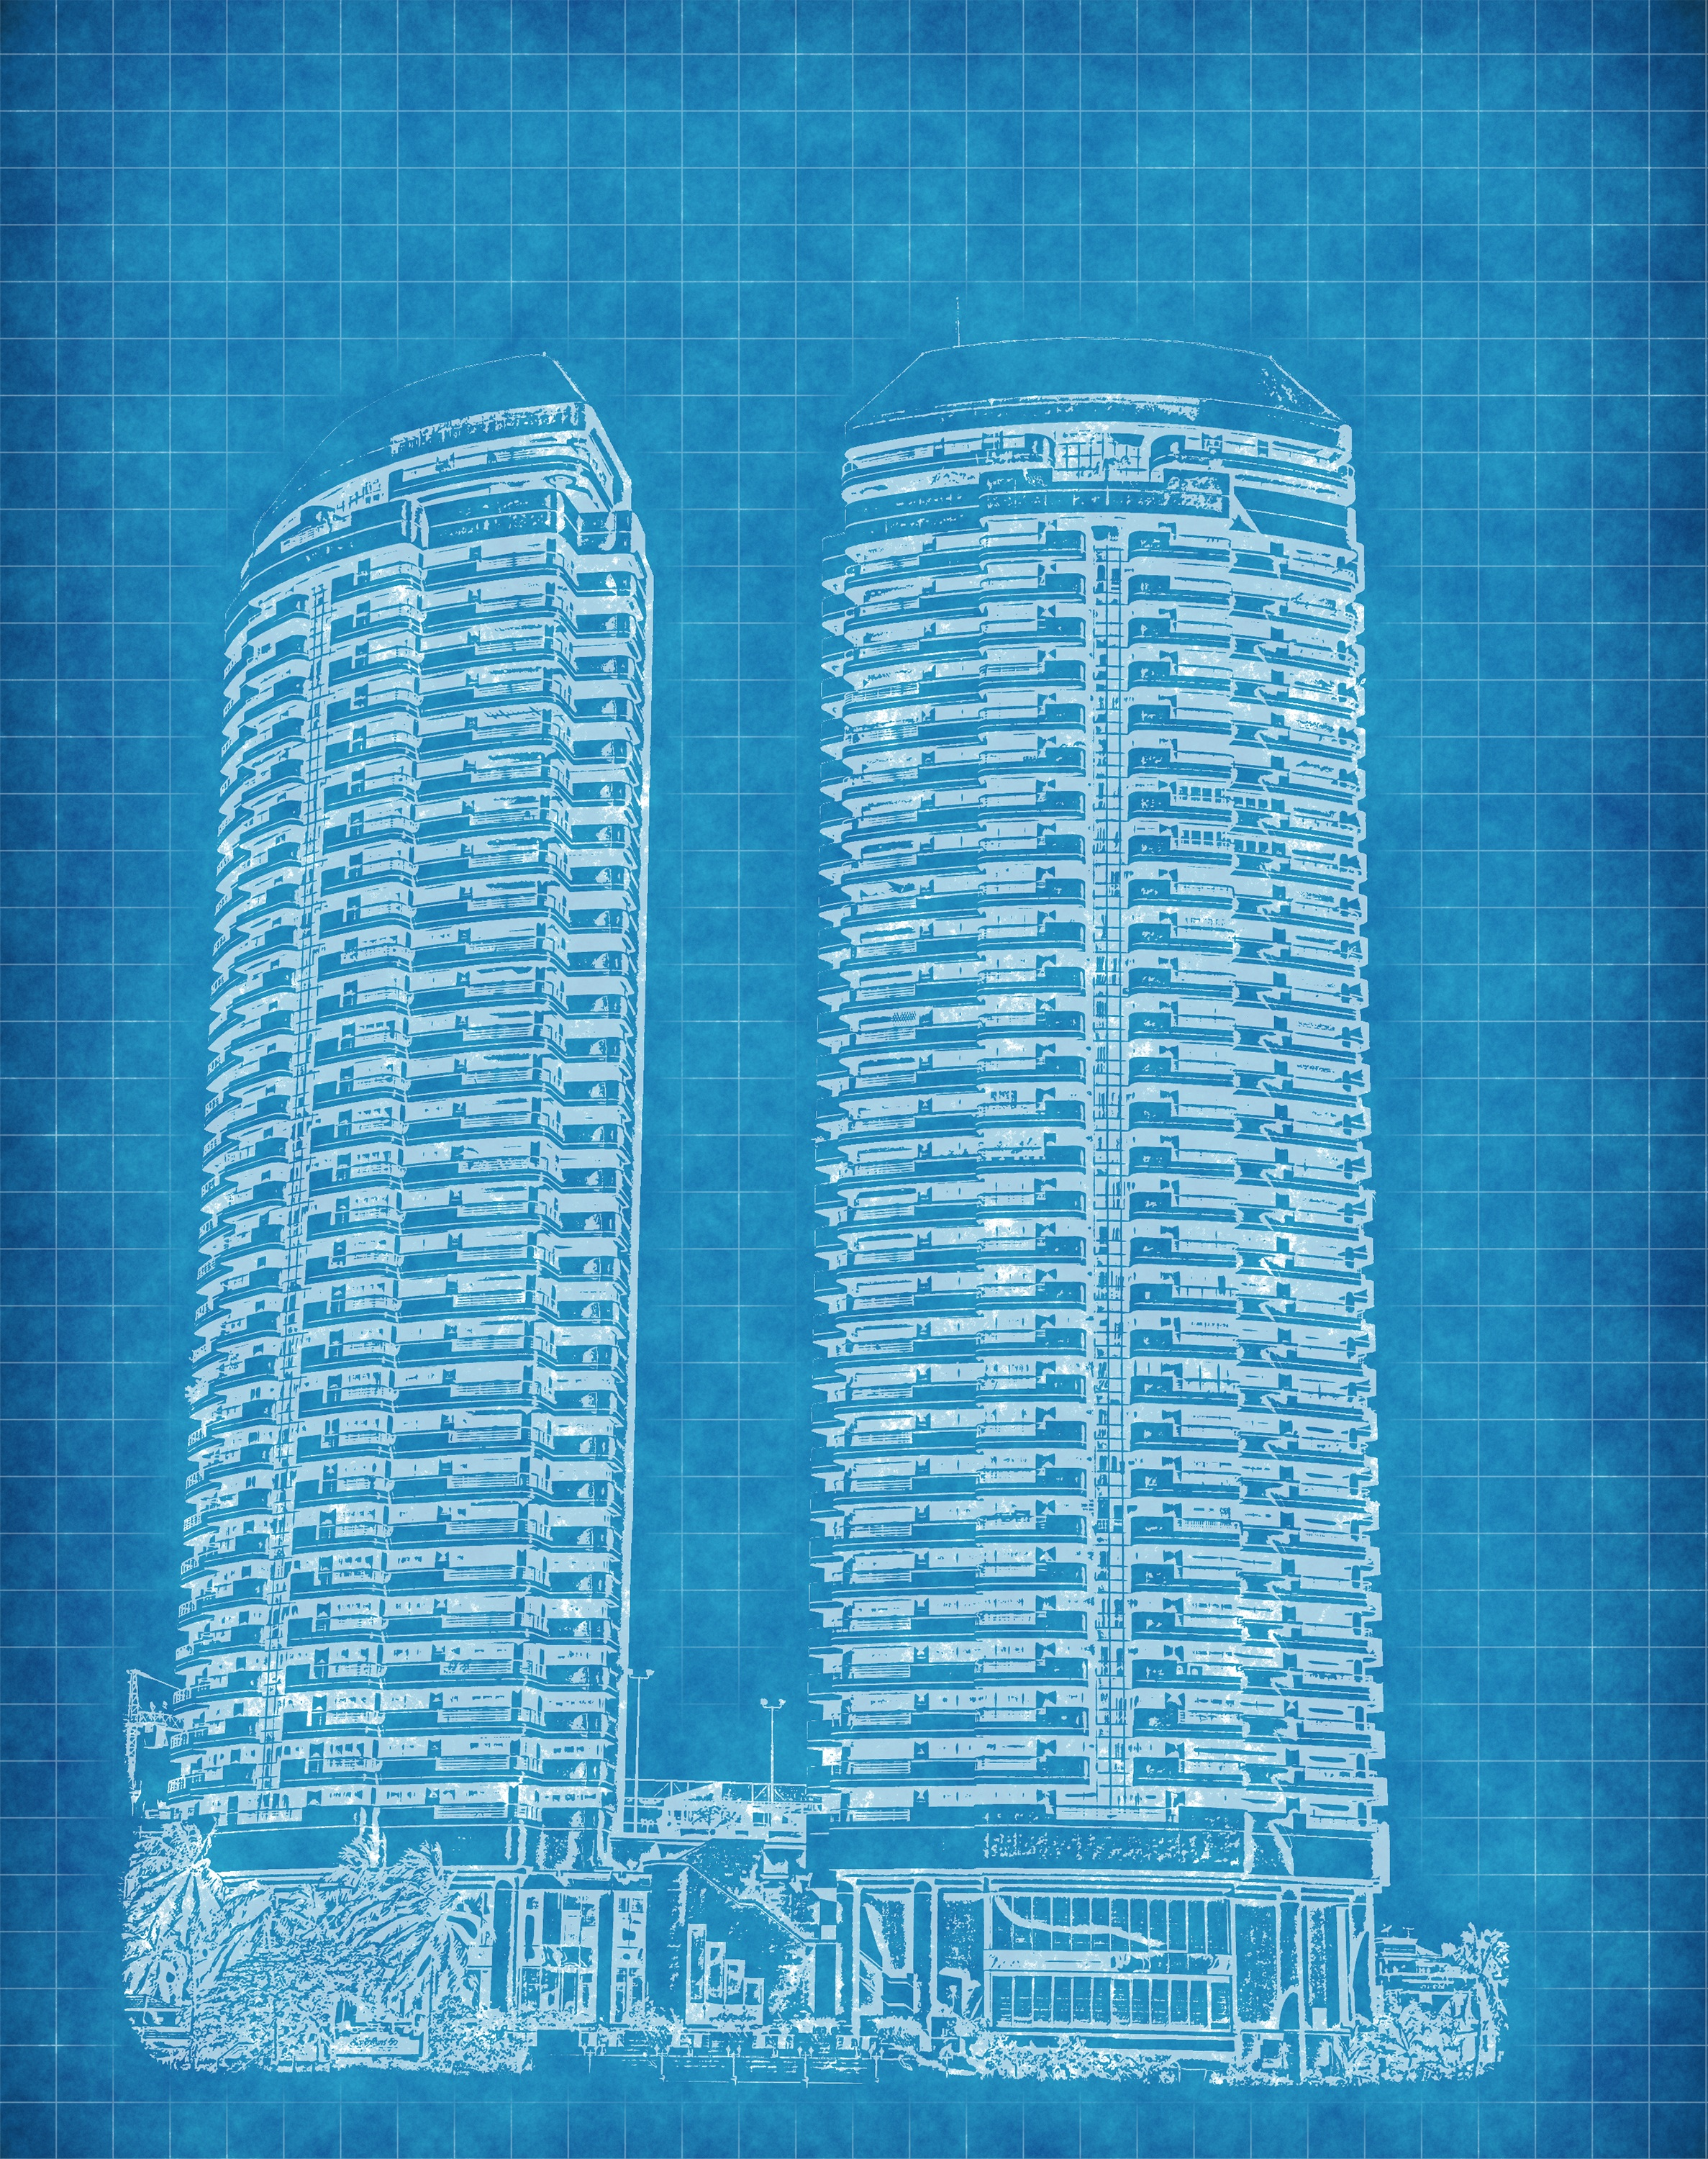
\includegraphics[width=\paperwidth,height=\paperheight]{image/blueprint}
        };
    \end{tikzpicture}
}

\chapter{But du portfolio}
\label{chap:but_portfolio}

\section{Cadre formel et ancrage théorique}

Le présent portfolio d'apprentissage s'érige dans le cadre du Master HES-SO Innokick, au sein du module de Différenciation Métier (MDM), en vue de la validation des 6 crédits ECTS qui lui sont associés. Ce travail a été échafaudé sous la supervision de Bastien Petitpierre, professeur référent, durant l'année académique 2025-2026.

\subsection*{Question structurante du portfolio}

Le présent travail s'organise autour d'une question unique, formulée en début de rédaction et tenue tout au long du document :

\begin{quote}
\itshape
Comment un ingénieur logiciel, formé à la résolution technique de problèmes, peut-il documenter avec rigueur le développement de compétences situées \emph{au-delà du code}, et démontrer leur mobilisation effective dans des situations professionnelles complexes ?
\end{quote}

Cette question oriente trois choix structurants : la sélection délibérée de trois compétences (A2, B4, C2) dont le développement marque la rupture la plus nette avec le profil initial ; la mobilisation d'un terrain professionnel dense (TWIICE, dispositifs médicaux certifiés) susceptible de produire des traces auditables ; et l'adoption stricte du cadre Tardif comme grille d'évaluation des preuves. Le référentiel auquel se rattachent ces trois compétences, ainsi que le module dans lequel s'inscrit le présent travail, sont introduits ultérieurement, au chapitre~\ref{chap:pec_documents} (\emph{Repères institutionnels}) ; leur justification détaillée est conduite, quant à elle, à la section~\ref{sec:trois-competences-justification}. Chacun des chapitres qui suivent peut être lu comme une instruction partielle de cette question.

\citet{tardif2006} définit le portfolio d'apprentissage en ces termes :

\begin{quote}
    « Un échantillon de preuves, sélectionnées par l'élève ou par l'étudiant dans l'intention de rendre compte fidèlement des apprentissages réalisés au cours d'une période ou au terme de cette période, qui fournit les données nécessaires, celles-ci comprenant une autoévaluation, pour que soit porté un jugement judicieux et éthique sur le niveau de développement des compétences concernées, sur le degré de maîtrise des ressources pouvant être mobilisées et combinées, ainsi que sur l'étendue des situations dans lesquelles ce niveau de développement et ce degré de maîtrise sont susceptibles de se matérialiser. » \citep[p.~266]{tardif2006}
\end{quote}

Il ne s'agit donc pas d'un simple assemblage de documents, mais bien d'un récit étayé par des preuves, rendant compte d'une progression dans les apprentissages. L'étudiant que je suis, est appelé à identifier ses ressources, à démontrer la manière dont il les agence au sein de situations concrètes, et à porter un regard autoévaluatif sur son propre développement. Cette démarche s'inscrit dans le prolongement d'une pratique réflexive, telle que la conçoivent \citet{lafortune2001} :

\begin{quote}
    « C'est là ce que peut faire le praticien réflexif, c'est-à-dire, une personne capable de décrire et d'analyser sa pratique afin de la rendre plus efficace et de développer ses propres modèles d'intervention. » \citep[p.~68]{lafortune2001}
\end{quote}

C'est précisément sur ces deux piliers, documentaire et réflexif, que le présent portfolio a été bâti. Les sections qui suivent exposent successivement les fondations professionnelles antérieures à la formation, les objectifs poursuivis et la posture réflexive adoptée tout au long de la démarche.

\subsection*{Note méthodologique et choix de structure}

\textbf{Recours à l'intelligence artificielle.}
Ce document a été rédigé avec l'assistance de l'intelligence artificielle (principalement des modèles de génération de texte de type grand modèle de langage), utilisée comme appui d'échafaudage, de reformulation et de clarification. Cette démarche s'inscrit explicitement dans le respect de deux cadres de référence : d'une part, les principes directeurs pour une bonne administration de l'IA générative dans l'enseignement définis par la HES-SO \citep{hessoIA2025}, qui encadrent les conditions d'un usage académique légitime et transparent au sein de l'institution ; d'autre part, la Recommandation sur l'éthique de l'intelligence artificielle proposée par l'UNESCO \citep{unescoIA2022}, qui pose les principes fondamentaux d'un recours responsable, centré sur la dignité humaine, la transparence et la redevabilité. Concrètement, l'IA a été mobilisée pour dresser les plans de sections, consolider la formulation de passages complexes, vérifier la solidité des enchaînements argumentatifs et poser des pierres d'appui là où l'expression manquait de charpente. Dans tous les cas, les idées, les expériences relatées, les preuves sélectionnées ainsi que les liens établis avec le référentiel de compétences sont le fruit d'un travail d'analyse personnelle. L'IA n'a pas bâti le contenu à ma place : elle a agi comme un outil d'assistance à la mise en forme, de la même manière qu'un traitement de texte ou un correcteur orthographique soutient la rédaction sans s'y substituer.

\textbf{Choix de la structure du document.}
La structure de ce portfolio n'a pas été imposée strictement par le cadre pédagogique : elle résulte d'un choix délibéré, visant à bâtir une architecture cohérente entre les différentes dimensions de la démarche. Le document se déploie en sept chapitres, regroupés en quatre ensembles de lecture.

\begin{itemize}
    \item \textbf{Un socle d'ouverture} pose les fondations : le chapitre \emph{But du portfolio} expose le cadre formel, l'ancrage théorique, le profil initial et les objectifs poursuivis ; le chapitre \emph{Titre du portfolio} explicite le sens du titre retenu et la logique symbolique qui soutient l'ensemble du document ; le chapitre \emph{Contrat individuel d'apprentissage} formalise les engagements posés en début de formation.

    \item \textbf{Un seuil de cadrage institutionnel}, constitué du chapitre \emph{Repères institutionnels}, dont le rôle est délibérément liminaire : rappeler succinctement les textes de référence (PEC, descriptif MDM, document cadre) sans y développer d'analyse substantielle.

    \item \textbf{Le cœur démonstratif du portfolio} se déploie ensuite en deux strates complémentaires. \emph{Espace modules} assure une fonction de cartographie : il rend visibles les apprentissages, les ressources rencontrées et leur mise en perspective. \emph{Situations professionnalisantes et analyse des compétences} remplit une fonction probatoire : il documente, avec situations, traces et preuves détaillées, la démonstration des compétences A2, B4 et C2.

    \item \textbf{Un horizon d'ouverture}, enfin, constitué du chapitre \emph{Perspectives pour la suite}, ouvre le chantier des prolongements envisagés.
\end{itemize}

Cette architecture vise à donner à lire non seulement ce que j'ai appris, mais la trajectoire par laquelle ces apprentissages ont été construits.

Par ailleurs, afin de pallier une contrainte récurrente de la formation, à savoir la disponibilité parfois différée des supports de présentation des enseignants, j'ai fait le choix de décrire les ressources mobilisées ou de les reconstituer moi-même lorsque nécessaire. Ce choix reflète ma réalité d'apprentissage durant les cours : dans plusieurs situations, les supports étant transmis a posteriori, la compréhension s'est d'abord construite à partir de mes notes.

\section{Note méthodologique}
\label{sec:note-methodologique}

Cette section explicite les choix méthodologiques qui structurent le portfolio, conformément à l'attente d'un travail académique de niveau Master : critères de sélection, modes de production des preuves, traitement des biais.

\subsection*{Sélection des trois compétences}

Le module de Différenciation Métier, dont le cadre est présenté au chapitre~\ref{chap:pec_documents} (\emph{Repères institutionnels}), impose la sélection de trois compétences au sein du référentiel Innokick (une par famille A, B, C), lui-même introduit dans ce même chapitre. Trois critères ont guidé la sélection retenue (A2, B4, C2) :

\begin{enumerate}
    \item \textbf{Critère d'écart au profil initial.} La compétence retenue devait correspondre à une zone clairement sous-développée dans le profil d'ingénieur logiciel d'entrée en formation. Les compétences déjà bien établies (par exemple B6 \emph{Élaboration de roadmaps}, ancrée dans l'expérience professionnelle antérieure) ont été écartées, car elles n'auraient pas permis de documenter une \emph{progression}.
    \item \textbf{Critère de mobilisation effective.} La compétence devait avoir été réellement sollicitée dans une situation professionnelle complexe au cours de l'année, et avoir produit des artefacts datés susceptibles d'être interprétés comme preuves au sens de~\citet{tardif2006}.
    \item \textbf{Critère de cohérence d'ensemble.} Les trois compétences retenues devaient former un système cohérent, en convergeant vers une posture professionnelle identifiable (ici : architecture décisionnelle, à l'interface du technique et du stratégique).
\end{enumerate}

\subsection*{Sélection des situations professionnalisantes et des artefacts}

Pour chaque compétence retenue, une situation professionnelle principale a été choisie selon trois critères : (i) authenticité (situation réellement vécue, non simulée) ; (ii) complexité (présence d'une divergence ou d'un arbitrage non trivial) ; (iii) traçabilité (production d'au moins un artefact daté et auditable). L'encart d'authenticité en tête du chapitre \emph{Situations professionnalisantes et analyse des compétences} précise, pour chaque artefact mobilisé, sa date de production, son contexte d'origine, sa version et son statut.

Une situation secondaire \emph{intra-Innokick} (atelier de prototypage en groupe) est mobilisée pour la compétence A2 afin d'éprouver la \emph{transférabilité} du développement de cette compétence hors du terrain principal TWIICE.

\subsection*{Mode de production des autoévaluations chiffrées}

Les scores avant/après formation (radars du \emph{Bilan de progression}) sont des autoévaluations \emph{reconstituées a posteriori}, calibrées sur la grille de descripteurs Tardif (\emph{découvrir → appliquer → mobiliser → transmettre}, reproduite en tête du bilan). Trois précautions méthodologiques sont assumées :

\begin{itemize}
    \item Les scores « avant » n'ont pas été produits en début d'année puis archivés : ils sont une lecture réflexive de l'écart parcouru, non une mesure indépendante du temps t-0. Cette limite est explicitement documentée dans le chapitre dédié.
    \item Les scores « après » sont ancrés, dans la mesure du possible, à des artefacts vérifiables (preuves probatoires mobilisées dans le chapitre \emph{Situations}).
    \item Aucune triangulation par un tiers (pair, enseignant, hiérarchie) n'est intégrée au corps du portfolio ; les sources de triangulation externes disponibles (historique GitLab, comptes-rendus signés, validations hiérarchiques) sont listées en tête du chapitre \emph{Situations} et communicables à l'examinateur sur demande motivée.
\end{itemize}

\subsection*{Traitement des biais et des limites}

Quatre biais sont explicitement assumés dans ce travail :

\begin{itemize}
    \item \textbf{Biais rétrospectif} des scores « avant », typique des autoévaluations a posteriori (cf.~encart dédié dans le \emph{Bilan de progression}).
    \item \textbf{Concentration sur un terrain unique (TWIICE)} pour deux des trois compétences (B4 et C2). Cette limite est posée comme constat ; elle est partiellement compensée par l'introduction d'un second contexte pour A2 (atelier prototypage Innokick).
    \item \textbf{Pivot rétrospectif du 3\textsuperscript{e} critère du contrat d'apprentissage} (design / lecture de marché -> \emph{couche de pilotage orientée valeur} [\textit{business layer}]), documenté et argumenté dans le chapitre \emph{Perspectives}, mais sans note de pivot horodatée en cours d'année (cf.~annexe dédiée).
    \item \textbf{Usage de l'intelligence artificielle générative} dans la rédaction, déclaré dans la sous-section précédente et instrumenté en annexe~\ref{annex:usage-ia} (modèles, périmètre d'usage, périmètre d'exclusion, dispositif de vérification).
\end{itemize}

Ces biais ne sont pas considérés comme des défauts à dissimuler, mais comme des éléments constitutifs du dispositif méthodologique : leur explicitation participe de l'exigence de probité attendue d'un travail réflexif au sens de~\citet{schon1994} et~\citet{perrenoud2001}.

\section{Ancrage professionnel initial}

Ingénieur logiciel\footnote{Un \textbf{ingénieur logiciel} est un professionnel qui conçoit, développe, teste, déploie et maintient des \textbf{logiciels} : c'est-à-dire des programmes informatiques (suites d'instructions exécutées par une machine) destinés à automatiser une tâche, traiter de l'information ou piloter un système. À la différence du simple développeur, l'ingénieur logiciel applique une démarche \textbf{d'ingénieur} : analyse formelle d'un besoin, choix raisonné d'une architecture, prise en compte des contraintes de fiabilité, de performance, de sécurité et de coût, et capacité à justifier ses décisions techniques. Le terme « ingénieur » désigne ici plus largement un professionnel formé à résoudre des problèmes complexes par une approche méthodique et quantifiée, en s'appuyant sur des connaissances scientifiques et des standards reconnus.\label{fn:ingenieur-logiciel}} de formation, diplômé de la Haute École d'Ingénierie et de Gestion du Canton de Vaud (HEIG-VD\footnote{La \textbf{HEIG-VD} (Haute École d'Ingénierie et de Gestion du Canton de Vaud) est une école d'ingénieurs et de gestion membre de la HES-SO, située à Yverdon-les-Bains. Elle délivre notamment des Bachelors of Science HES-SO en ingénierie (informatique, électricité, microtechnique, etc.) et en économie d'entreprise.}), mon parcours professionnel s'est édifié à travers plusieurs secteurs qui ont chacun posé une pierre à ma posture actuelle.

J'ai d'abord exercé dans le secteur industriel, où j'ai été chargé d'automatiser la récolte de données d'une chaîne de production. Cette expérience m'a ancré dans les réalités opérationnelles du terrain : contraintes de cadence, fiabilité des systèmes, nécessité d'architecturer\footnote{Le verbe \emph{architecturer}, employé ici dans son acception technique, désigne l'acte de concevoir et d'organiser structurellement un système logiciel ou matériel : définir ses composants, leurs responsabilités et leurs interactions de manière cohérente, robuste et évolutive.} des solutions robustes et immédiatement exploitables. Elle m'a également sensibilisé aux enjeux de communication entre les équipes techniques et les opérateurs de production.

J'ai ensuite intégré le secteur bancaire, au sein du département reporting\footnote{Le \emph{département reporting} d'une banque privée est chargé de produire les rapports financiers réglementaires et commerciaux destinés aux clients, aux régulateurs et à la direction : relevés de portefeuille, rapports de performance, déclarations fiscales et documents de conformité. Il opère à l'intersection des contraintes légales, des exigences des autorités de surveillance (FINMA, en contexte suisse) et des attentes des clients fortunés.\label{fn:reporting}} d'une banque privée. Dans cet environnement, j'ai été confronté aux enjeux de conformité réglementaire, à la coordination entre entités géographiquement distribuées et à la nécessité de produire des livrables\footnote{Un \textbf{livrable} (\emph{deliverable}) désigne tout produit, document ou artefact formellement remis à un destinataire (client, partie prenante, autorité réglementaire) au terme d'une activité ou d'un jalon de projet. En contexte logiciel et d'ingénierie, un livrable peut être un programme exécutable, un rapport, une spécification, un plan de tests, un dossier de conformité, etc. Il est généralement défini par un cahier des charges, soumis à des critères d'acceptation et tracé jusqu'à sa validation.\label{fn:livrable}} fiables sous contraintes strictes de présentation et de légalité. C'est dans ce contexte que j'ai perçu, pour la première fois, les fissures d'une approche exclusivement technique : mes propositions d'amélioration, bien que pertinentes sur le plan opérationnel, manquaient de charpente et de capacité de conviction auprès des parties prenantes.

J'ai également évolué brièvement dans l'industrie des systèmes audiovisuels, où je développais des interfaces de pilotage pour des équipements techniques. Bien que de courte durée, cette expérience m'a révélé l'importance cruciale de la compréhension des besoins utilisateurs en amont du développement. J'y ai posé les premières pierres, de manière empirique et sans plan méthodologique formel, d'une pratique du prototypage et de la validation par l'usage.

J'exerce désormais au sein de TWIICE, entreprise spécialisée dans la conception de dispositifs robotiques à visée médicale. Mes responsabilités portent principalement sur le développement des différents logiciels embarqués\footnote{Dans ce contexte, les \emph{logiciels embarqués} désignent les programmes s'exécutant directement sur les composants matériels de l'exosquelette (microcontrôleurs, processeurs embarqués). Ils sont responsables du pilotage en temps réel des actionneurs, de l'acquisition des données issues des capteurs, de la gestion de l'alimentation ainsi que de la communication entre les différents modules électroniques du dispositif médical, par contraste avec les logiciels tournant sur des serveurs distants ou des applications mobiles.}, l'architecture\footnote{Le terme \emph{architecture}, employé ici dans son acception informatique, désigne l'organisation structurelle du système logiciel : la manière dont les différents composants logiciels sont découpés, agencés et mis en relation, ainsi que les décisions techniques qui régissent leurs interactions (protocoles de communication, interfaces, gestion des états). Dans le contexte de TWIICE, cela recouvre notamment la définition des flux de données entre le calculateur central, les cartes de contrôle moteur et l'interface utilisateur embarquée.} des communications entre eux ainsi que la mise en œuvre des conformités normatives en vigueur (IEC~62304\footnote{L'\emph{IEC~62304} \citep{iec62304} est une norme internationale qui définit les exigences relatives aux processus du cycle de vie des logiciels de dispositifs médicaux : développement, maintenance, gestion des risques logiciels et traçabilité. Elle est obligatoire pour tout logiciel intégré dans un dispositif médical mis sur le marché européen.\label{fn:iec62304}}, MDR\footnote{Le \emph{MDR} (\textit{Medical Device Regulation}, \citealp{mdr2017}) est le règlement européen sur les dispositifs médicaux, entré en application en mai 2021. Il remplace la directive MDD et renforce les exigences en matière de sécurité, de performance clinique, de surveillance post-marché et de traçabilité des dispositifs médicaux commercialisés dans l'Union européenne.}). Ce contexte, à la fois techniquement exigeant et fortement réglementé, a consolidé l'édifice de mon autonomie professionnelle.

C'est la convergence de ces expériences qui m'a conduit à un constat récurrent : il existe, entre l'étage technique dans lequel j'évolue avec aisance et l'étage métier où se décident la vision, la stratégie et la valeur d'un projet, un plafond de verre\footnote{\textbf{Note terminologique.} L'expression \emph{plafond de verre} (\textit{glass ceiling}) désigne, dans la littérature sociologique anglo-saxonne depuis les années 1980, les barrières invisibles qui freinent l'accès des femmes et des minorités aux positions de direction. L'emploi qui en est fait ici constitue un \emph{déplacement métaphorique assumé} vers la sphère des barrières de compétence personnelle : je conserve le mot pour son économie d'image (limite invisible mais étanche), tout en reconnaissant qu'il ne désigne pas, dans le présent portfolio, le concept sociologique d'origine. Le lecteur pourra y lire, plus précisément, un \emph{plafond de compétence transdisciplinaire}.\label{fn:plafond-verre}}. Je suis capable de concevoir, de développer et de livrer des solutions techniques robustes, mais je me heurte systématiquement à cette cloison invisible dès qu'il s'agit de contribuer pleinement au projet dans sa dimension globale.

Dans l'industrie, je pouvais automatiser une chaîne de production, mais je n'avais pas les clés pour défendre la valeur ajoutée de cette automatisation auprès de la direction. En banque, mes propositions d'amélioration étaient techniquement solides, mais elles ne franchissaient pas le seuil de la décision, faute de savoir les charpenter et les présenter de manière convaincante. Dans l'audiovisuel, j'ai entrevu l'importance du prototypage et de l'empathie utilisateur, sans disposer des plans méthodologiques pour formaliser cette intuition.

Ce plafond se manifeste toujours par les mêmes brèches dans mon profil : la capacité à concevoir des interfaces intelligibles et désirables, l'analyse de marché permettant d'identifier les besoins et les opportunités, l'aptitude à présenter et à défendre un projet de manière convaincante, ainsi que la compétence à déléguer et à collaborer au sein d'une équipe pluridisciplinaire. Sans ces compétences, je reste cloisonné dans le rôle d'exécutant technique, incapable de porter pleinement ma contribution à la création de valeur.

C'est cette prise de conscience, mûrie au fil de plusieurs années et de contextes professionnels variés, qui m'a conduit à m'engager dans la formation Innokick, avec l'intention de briser ce plafond et de bâtir une professionnalité plus complète.

\section{Objectifs du portfolio}

Conformément au cadre théorique posé par~\cite{tardif2006}, le présent portfolio vise à documenter l'élévation de ma trajectoire de développement à travers les six phases du Design Thinking (empathie, définition, idéation, prototypage, test, implémentation). De manière plus spécifique, il poursuit trois objectifs :

\begin{itemize}
    \item \textbf{Identifier les apprentissages érigés} au fil de chaque phase, en particulier dans des domaines éloignés de mon expertise initiale : la gestion des divergences et la facilitation collective (A2), la mise en œuvre de méthodes agiles dans un contexte réglementé (B4), ou encore la synthèse de problématiques complexes sous contrainte de certification (C2).
    \item \textbf{Rendre visibles les nouvelles ressources} progressivement maîtrisées : connaissances théoriques, méthodes (veille stratégique, prototypage, protocoles de validation), attitudes (ouverture, esprit critique), valeurs et schèmes d'action.
    \item \textbf{Démontrer l'assemblage et la combinaison de ces ressources} au sein de situations concrètes, qu'elles soient issues de la formation Innokick ou de mon contexte professionnel chez TWIICE.
\end{itemize}

Cette démarche illustre un parcours développemental structuré en trois niveaux : les fondations professionnelles acquises à l'entrée en formation, les transformations engagées en cours de cursus, et l'édifice professionnel visé à terme.

\section{Trois compétences, trois chantiers}
\label{sec:trois-competences-justification}

Le cadre académique du module de Différenciation Métier (MDM) du Master Innokick, dont la présentation détaillée fait l'objet du chapitre~\ref{chap:pec_documents} (\emph{Repères institutionnels}), impose une contrainte structurante : il ne s'agit pas de balayer l'intégralité des dix-huit compétences du référentiel Innokick, mais d'en \textbf{sélectionner trois}, une par famille, et d'en documenter le développement avec rigueur et profondeur. Les trois familles, dont le détail est également exposé au chapitre~\ref{chap:pec_documents}, sont les suivantes :

\begin{itemize}
    \item \textbf{Famille A} : Compétences sociales et personnelles
    \item \textbf{Famille B} : Compétences méthodologiques
    \item \textbf{Famille C} : Compétences métier
\end{itemize}

Ce choix n'est pas arbitraire. Il résulte d'une démarche réflexive : identifier, parmi les dix-huit compétences du référentiel, celles dont le développement illustre le mieux la rupture entre le profil que j'étais en entrant en formation et celui que j'ambitionne d'être. Chaque compétence retenue correspond à un étage structurant de cet édifice en construction, à un endroit précis où la formation a ébranlé une certitude, ouvert une brèche ou posé une poutre que l'intuition seule n'aurait pas suffi à dresser.

Les trois chantiers retenus sont :

\begin{description}
    \item[\textbf{A2 : Gestion des divergences et facilitation de la convergence}] \hfill \\
    Cette compétence incarne la rupture la plus profonde avec ma posture initiale d'ingénieur. Là où l'expert tend à trancher, à imposer une direction ou à défendre sa solution, le praticien compétent en A2 crée les conditions pour que le groupe converge par lui-même vers une décision partagée. Acquérir cette compétence, c'est ériger un étage entièrement nouveau : celui de la facilitation, de la médiation et de l'intelligence collective. C'est précisément là que se situe l'une des brèches les plus saillantes de mon profil initial, et c'est pourquoi ce chantier est au cœur de ce portfolio.

    \item[\textbf{B4 : Méthodes agiles au service du prototypage itératif}] \hfill \\
    Connaître une méthode est une chose ; savoir l'adapter à un contexte contraint en est une autre. La compétence B4 ne se réduit pas à la maîtrise de Scrum ou du Lean : elle exige de comprendre \emph{pourquoi} une méthode fonctionne, pour pouvoir la moduler quand le terrain impose ses propres contraintes. Pour un ingénieur qui aspire à dépasser le registre de l'exécution technique, cette capacité à piloter un processus itératif avec méthode et discernement constitue un pilier central de la professionnalité visée.

    \item[\textbf{C2 : Synthèse et définition des problématiques prioritaires}] \hfill \\
    La capacité à \emph{nommer le bon problème} avant de chercher une solution est l'une des marques les plus distinctives du professionnel de l'innovation. Cette compétence incarne le passage du technicien qui répond à la question posée au praticien qui s'assure d'abord que la bonne question est posée. Elle constitue la clé de voûte de l'édifice : sans une problématique bien définie, ni la créativité ni la rigueur méthodologique ne peuvent s'exercer pleinement.
\end{description}

\section{Le portfolio comme outil réflexif}

Au-delà de sa dimension certificative, ce portfolio constitue avant tout un instrument d'apprentissage et d'autorégulation. En conservant des traces structurées de mes réflexions, de mes réussites comme de mes difficultés, il me permet d'inspecter ma progression et d'ajuster ma démarche de manière continue.

Cette pratique réflexive s'appuie sur un questionnement métacognitif régulier, échafaudé autour des interrogations suivantes :

\begin{itemize}
    \item Quels savoirs ai-je acquis à travers ce cours, cette lecture, cette expérience ?
    \item En quoi ces apprentissages consolident-ils ou reconfigurent-ils ma manière de penser et d'agir ?
    \item Quelles conséquences en découlent sur ma façon de collaborer et d'exercer ma professionnalité ?
    \item Quels étages nouveaux vais-je ériger, et selon quelles modalités ?
\end{itemize}

Le portfolio se conçoit ainsi comme un chantier permanent d'interrogation de mes pratiques, de confrontation de mes intuitions aux cadres théoriques, et d'édification progressive d'une posture professionnelle qui s'élève au-delà du registre strictement technique.

\clearpage
\ClearShipoutPictureBG

\chapter{Titre du portfolio : Au-delà du code}
\label{chap:titre_portfolio}

% Justification du titre et réflexion sur le fil rouge du parcours.

\clearpage

\AddToShipoutPictureBG{
    \begin{tikzpicture}[remember picture, overlay]
        \node[opacity=0.08] at (current page.center) {
            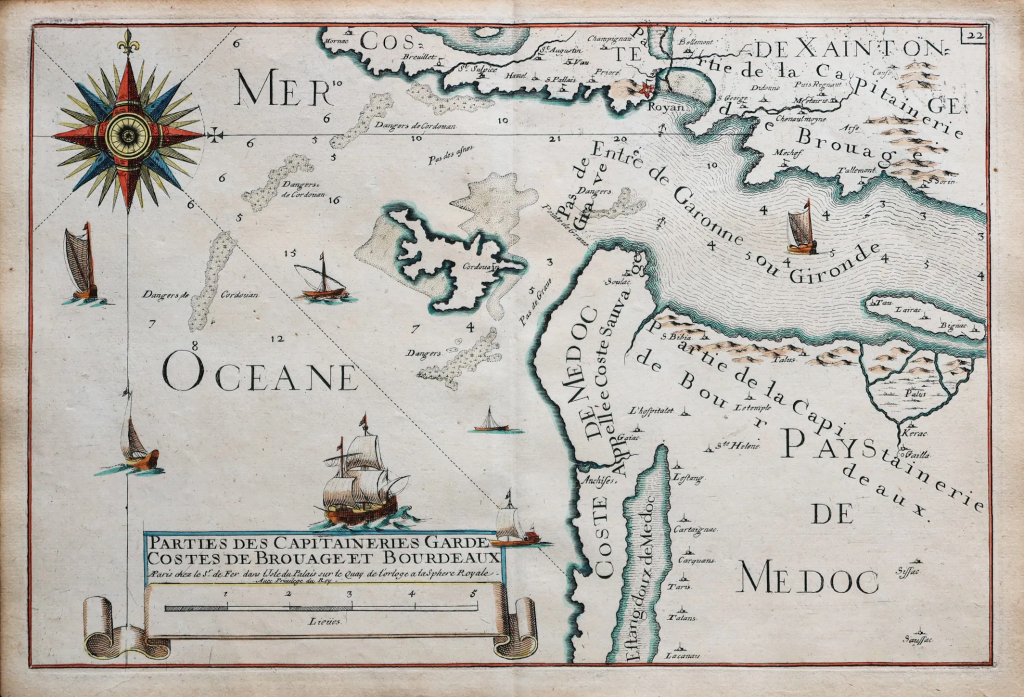
\includegraphics[width=\paperwidth,height=\paperheight]{image/carte-maritine}
        };
    \end{tikzpicture}
}

\chapter{Contrat individuel d'apprentissage}
\label{chap:contrat_apprentissage}

Le contrat individuel d'apprentissage, établi au commencement de l'année académique et validé par le professeur référent, constitue la carte de navigation de la démarche présentée dans ce portfolio. Sa version intégrale est jointe en \textbf{annexe A}. Le présent chapitre n'en reproduit pas le détail ; il en expose les lignes directrices, les choix déterminants et leur cohérence avec les compétences retenues.

\section{Cap pédagogique et compétences retenues}

Le cap pédagogique fixé au début du parcours repose sur une finalité claire : dépasser le registre strictement technique pour évoluer vers une professionnalité transdisciplinaire, capable d'articuler conception, collaboration, cadrage stratégique et mise en œuvre.

Dans cette perspective, trois compétences ont été arrimées comme points d'ancrage. Leur justification détaillée est présentée dans l'introduction, à la section \textit{Trois compétences, trois chantiers} (voir section~\ref{sec:trois-competences-justification}) :

\begin{itemize}
    \item \textbf{A2} (gestion des divergences et facilitation de la convergence), pour renforcer la délégation, la coopération et la prise de décision collective.
    \item \textbf{B4} (méthodes agiles au service du prototypage itératif), pour structurer l'apprentissage par la pratique et piloter les itérations avec méthode.
    \item \textbf{C2} (synthèse et définition des problématiques prioritaires), pour affiner la capacité à poser un diagnostic pertinent avant d'orienter une réponse.
\end{itemize}

Ces trois compétences forment la quille du parcours développemental : elles soutiennent la progression attendue et assurent une cohérence entre intentions initiales, activités de formation et critères d'autoévaluation.

\section{Logique d'alignement entre objectifs et choix de cours}

Mes objectifs pédagogiques personnels se concentrent sur trois axes :

\begin{itemize}
    \item développer une conception centrée utilisateur et une meilleure lisibilité des solutions proposées ;
    \item améliorer la capacité à défendre un projet, à argumenter sa valeur et à l'inscrire dans une logique de marché ;
    \item progresser dans la collaboration, la délégation et la conduite collective des projets.
\end{itemize}

Le choix des cours à option répond directement à cet agencement d'objectifs et fait écho aux compétences justifiées dans l'introduction :

\begin{description}
    \item[\textbf{Méthode de recherche 1, 2 et 3}] repère analytique pour investiguer le terrain, clarifier les besoins et nourrir prioritairement la compétence \textbf{C2}.
    \item[\textbf{Médiation}] appui central pour traiter les divergences, parvenir à des accords opératoires et renforcer la compétence \textbf{A2}.
    \item[\textbf{Gestion de projet 1, 2 et 3}] cadre méthodologique pour conduire des cycles itératifs et consolider la compétence \textbf{B4}.
    \item[\textbf{Gestion financière 1 et 2}] appui de pilotage pour relier faisabilité économique, arbitrages de projet et argumentation auprès des décideurs, en soutien transversal des trois compétences.
    \item[\textbf{Technique de vente et négociation}] deux compétences que mon profil d'ingénieur n'a jamais cultivées, mais indispensables pour défendre la valeur d'une solution, convaincre des décideurs et négocier dans des contextes professionnels. Ces cours comblent directement la brèche entre l'expertise technique et la capacité à la valoriser.
    \item[\textbf{Start-up et industrialisation}] pont entre l'intuition entrepreneuriale acquise sur le terrain et un cadre structuré pour penser le passage d'une idée à un produit viable ; ancrage dans la réalité des deux univers que j'ai traversés.
    \item[\textbf{Droit des sociétés et protection intellectuelle}] deux angles d'un même angle mort : ne pas savoir cadrer juridiquement une initiative ou protéger ce qu'on crée est un frein réel à toute ambition de dépasser le rôle d'exécutant. Ces cours apportent les fondations manquantes.
    \item[\textbf{Communication au sein d'une institution}] compétence éprouvée sous sa face la plus difficile lors de restructurations subies ; comprendre ses mécanismes pour ne plus en être le simple objet mais un acteur capable d'y naviguer.
    \item[\textbf{Méthode de veille}] domaine qui me passionne depuis que j'ai mis en place des outils d'aide à la décision stratégique ; l'approfondir nourrit directement la compétence \textbf{C2} et la capacité à cadrer les bons problèmes.
    \item[\textbf{Prototypage et produit physique}] lacune assumée d'un ingénieur logiciel : penser par le faire, avec des contraintes matérielles, change profondément la manière d'innover et d'itérer.
    \item[\textbf{Vidéo et art oratoire}] deux compétences de communication au service de la même finalité : donner corps à une idée, la rendre lisible et convaincante. L'art oratoire en particulier, bien qu'abordé avec réticence, répond à un besoin réel d'assurance en expression orale face à des décideurs.
\end{description}

Ainsi, la logique d'ensemble est explicitement alignée : les objectifs de formation fixent le cap, les compétences A2, B4 et C2 en tracent la route, et les cours retenus constituent les moyens opérationnels pour tenir ce cap.

\section{Critères de progression}

Les critères formulés ci-dessous reflètent le point de vue au moment de la rédaction du contrat, en début d'année académique. Ils ont servi de boussole initiale. Comme le chapitre \textit{Perspectives pour la suite} le documente, la trajectoire réelle a partiellement déplacé certaines priorités : en particulier, le troisième critère, centré sur le design et la lecture de marché, a progressivement cédé la place à un axe plus marqué vers la gouvernance de projet et le passage à la \emph{couche de pilotage orientée valeur} (\textit{business layer}). Ce glissement n'est pas un écart à corriger, mais le signe d'un parcours réflexif vivant, où les priorités se précisent à mesure que la formation révèle des leviers plus déterminants pour la trajectoire visée.

La progression est appréciée selon un double principe : validation externe (pairs et enseignants) et balises internes d'évolution. Les indicateurs privilégiés sont les suivants :

\begin{itemize}
    \item capacité à contribuer au-delà de l'exécution technique, notamment dans le cadrage des problèmes et la conduite de décisions partagées ;
    \item amélioration observable de la qualité des interactions collectives, de la délégation et de la coordination interdisciplinaire ;
    \item aisance accrue dans les dimensions antérieurement moins maîtrisées, en particulier le design, l'argumentation de valeur et la lecture de marché.
\end{itemize}

Cette trajectoire d'apprentissage ne s'est pas imposée d'elle-même : elle résulte d'un cap délibérément choisi, d'une lecture lucide des lacunes à combler et d'une volonté de naviguer vers des eaux jusqu'alors inexplorées. C'est cette même intention qui irrigue l'ensemble du portfolio et que les chapitres suivants s'attachent à documenter, étape par escale.

\clearpage
\ClearShipoutPictureBG

\clearpage

\AddToShipoutPictureBG{
    \begin{tikzpicture}[remember picture, overlay]
        \node[opacity=0.08] at (current page.center) {
            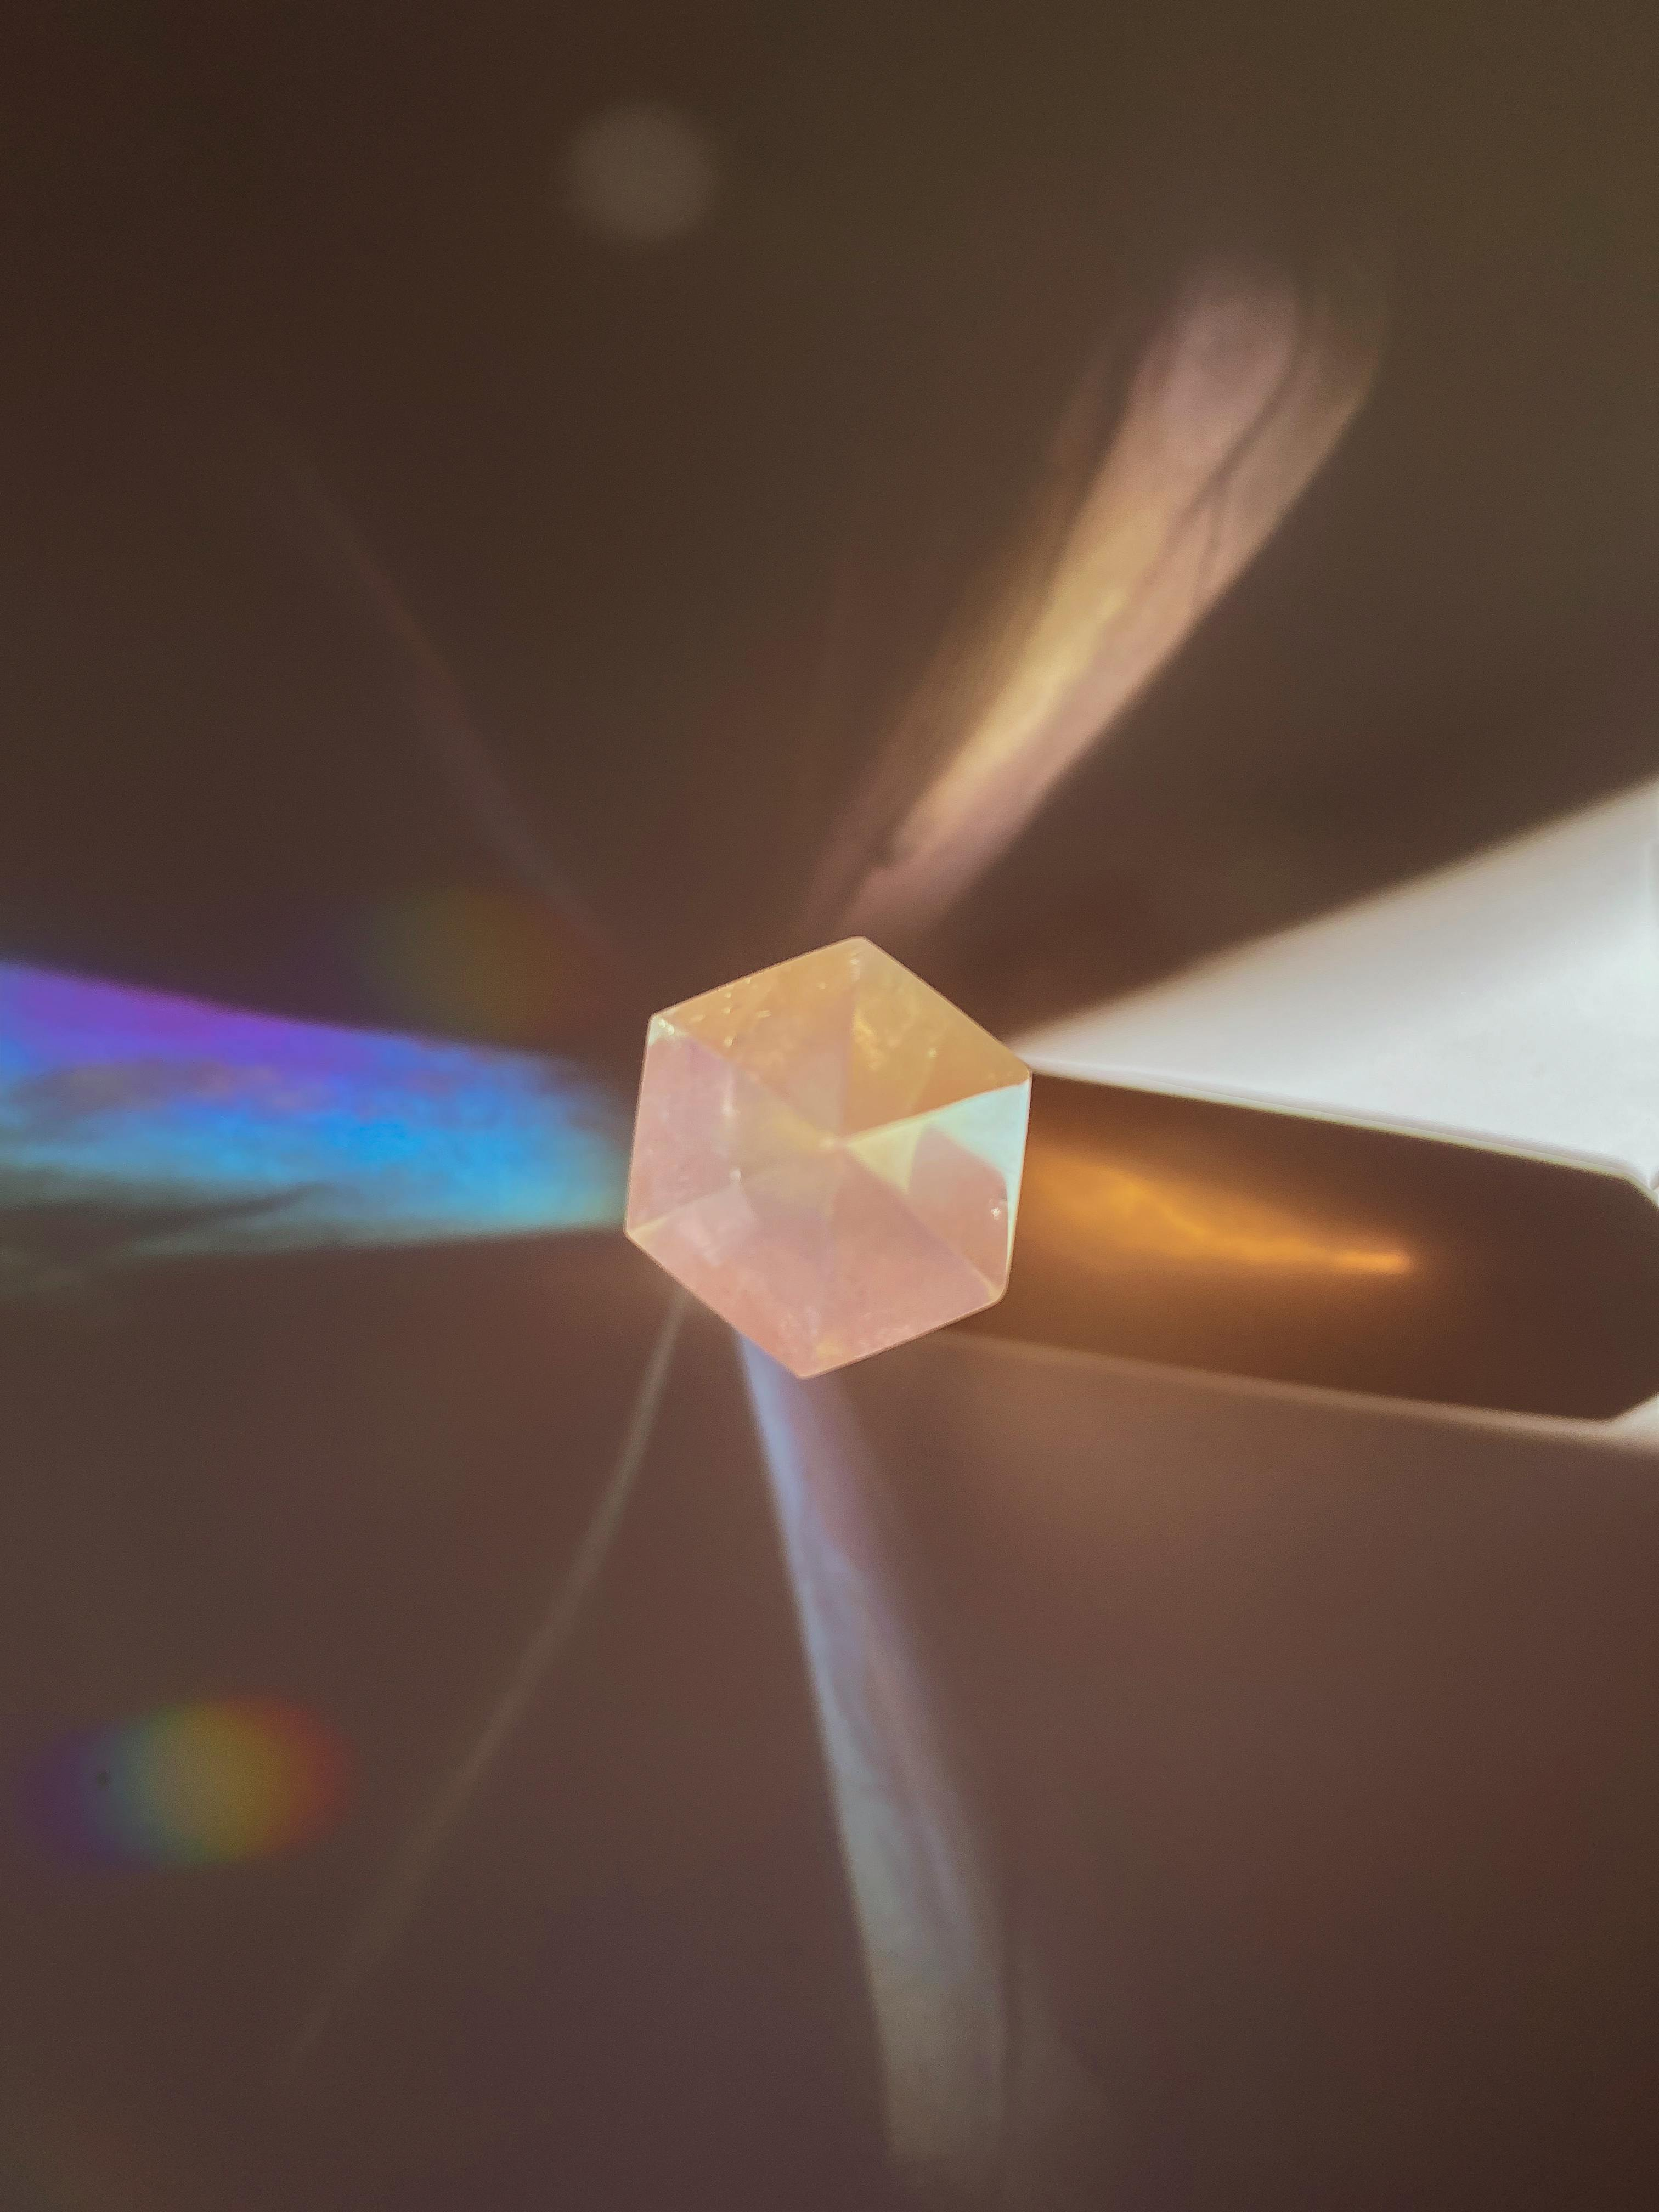
\includegraphics[width=\paperwidth,height=\paperheight]{image/prisme}
        };
    \end{tikzpicture}
}


\chapter{Repères institutionnels}
\label{chap:pec_documents}


\section{Fonction de ce chapitre dans l'économie du portfolio}

Ce chapitre assume une fonction délibérément liminaire : il ne constitue pas un bloc analytique autonome, mais un espace de cadrage destiné à projeter un premier éclairage sur les textes qui ont orienté la construction de ce portfolio. Situé à l'interface entre le contrat d'apprentissage et les chapitres démonstratifs, il n'a pas vocation à développer une analyse supplémentaire, mais à rendre perceptible l'horizon normatif au sein duquel la réflexion prend forme.

Autrement dit, il ne s'agit pas ici d'ajouter une strate interprétative de plus, mais de disposer, sous une lumière sobre et méthodique, les principaux textes qui ont servi de balises : cadre du programme, attendus du module et consignes propres à l'exercice. Leur rappel succinct vise moins l'exhaustivité que la lisibilité : il s'agit d'éclairer le point d'appui institutionnel du travail avant d'en exposer les développements analytiques.

\section{Documents de référence mobilisés}

Les documents ci-dessous ont servi de repères de cadrage tout au long de la rédaction.

\subsection*{Plan d'Études Cadre (PEC)}

Le Plan d'Études Cadre du Master HES-SO Innokick (version juillet 2024, annexe~\ref{annex:pec-innokick}) fixe la vision d'ensemble du programme, ses finalités, son architecture modulaire ainsi que ses modalités de certification. Il constitue, à cet égard, la source première d'intelligibilité du dispositif de formation.

Le PEC définit un référentiel de \textbf{dix-huit compétences clés}, regroupées en trois catégories : compétences sociales et personnelles (famille A), compétences méthodologiques (famille B) et compétences métier de l'innovateur ou de l'innovatrice (famille C). Ces dix-huit compétences s'articulent autour des \textbf{six phases du Design Thinking} (empathie, définition, idéation, prototypage, test, implémentation) qui structurent également l'ensemble de ce portfolio. C'est à la lumière de ce référentiel que sont situés le module de Différenciation Métier, les compétences retenues (A2, B4 et C2) et, plus largement, l'inscription de ce travail dans une trajectoire de professionnalisation orientée vers l'innovation transdisciplinaire.

\subsection*{Descriptif de module : Différenciation métier (MDM)}

Le descriptif officiel du module de Différenciation Métier (MDM), dont la version intégrale est jointe en \textbf{annexe H} (voir annexe~\ref{annex:descriptif-mdm}), pose les fondements pédagogiques au sein desquels ce portfolio s'inscrit. Il précise que le module est doté de \textbf{6 crédits ECTS} et repose sur une pédagogie différenciée : l'étudiant·e cible ses apprentissages selon ses besoins réels, dans un format principalement à distance favorisant l'autonomisation. Les trois objectifs d'apprentissage principaux sont les suivants : développer ses connaissances et sa culture transdisciplinaires ; acquérir les bases nécessaires à la bonne compréhension des modules d'approfondissement ; être capable d'organiser ses activités d'apprentissage en fonction de ses besoins et de se confronter aux situations les plus constructives.

Ce cadre est pleinement cohérent avec la démarche adoptée dans ce portfolio : le choix de trois compétences ciblées (A2, B4, C2), la logique réflexive et auto-dirigée qui structure chaque chapitre, et l'articulation entre formation et contexte professionnel répondent directement à ces objectifs.

\subsection*{Document cadre du portfolio}

Rédigé par Bastien Petitpierre, le document cadre du portfolio explicite la méthodologie attendue et en ordonne les principales exigences. Il met en lumière la structure prescrite, les fondements théoriques mobilisés (Tardif, Lafortune \& Deaudin) ainsi que les critères d'évaluation appelés à orienter le jugement académique porté sur ce travail. Tout au long de la rédaction, il a constitué une ligne de visée constante : non un moule rigide, mais un foyer de référence à partir duquel chaque section a été calibrée.

\subsection*{Introduction au module}

L'introduction au module, dispensée en début de formation, a joué un rôle d'éclairage initial. Elle a permis de clarifier les enjeux du portfolio, de présenter le référentiel des dix-huit compétences Innokick et de jeter les premières lumières sur ce que signifie documenter, avec rigueur, un parcours développemental.

\begin{quote}
Ces documents relèvent du cadrage et non de la démonstration. Ils fournissent l'éclairage d'arrière-plan indispensable à l'intelligibilité du travail, mais c'est dans les chapitres suivants que se déploie l'analyse proprement dite, là où les apprentissages, les ressources mobilisées et les situations professionnalisantes viennent étayer le développement des compétences retenues.
\end{quote}


\clearpage
\ClearShipoutPictureBG
\clearpage

\AddToShipoutPictureBG{
    \begin{tikzpicture}[remember picture, overlay]
        \node[opacity=0.06] at (current page.center) {
            \includegraphics[width=\paperwidth,height=\paperheight]{image/plante}
        };
    \end{tikzpicture}
}

\chapter{Espace modules}
\label{chap:espace_modules}

\bigskip

\begin{tcolorbox}[colback=blue!6, colframe=blue!55!black, boxrule=0.5pt, arc=4pt,
  left=10pt, right=10pt, top=8pt, bottom=8pt,
  title={\textbf{\small Positionnement du chapitre dans la démonstration}},
  fonttitle=\small\bfseries, coltitle=white, attach boxed title to top left={yshift=-2mm, xshift=4mm},
  boxed title style={colback=blue!55!black, arc=3pt, boxrule=0pt}]
\small
Ce chapitre a une fonction de \textbf{cartographie des apprentissages}. Il rassemble les matériaux de formation (cours, lectures, productions intermédiaires) et montre comment ils ont été mobilisés au fil des phases du Design Thinking.

Il ne constitue pas, à lui seul, la démonstration probante des compétences retenues. La \textbf{démonstration détaillée par traces et preuves} est menée dans le chapitre \emph{Situations professionnalisantes et analyse des compétences}, où les acquis A2, B4 et C2 sont explicitement argumentés à partir de situations, d'artefacts et d'analyses réflexives.
\end{tcolorbox}

\bigskip

La présente section rassemble une sélection représentative des apprentissages dispensés au fil de la formation Innokick. Loin de prétendre à l'exhaustivité, elle réunit un échantillon de traces témoignant d'un engagement actif dans les modules suivis et d'une volonté délibérée d'inscrire ces savoirs dans une réflexion personnelle et une mise en perspective professionnelle.

% ------------------------------------------------------------------------------
\section{Semences théoriques}
% ------------------------------------------------------------------------------

Les notes prises durant les sessions, en présentiel ou en ligne, constituent les apports initiaux de chaque apprentissage. S'y ajoutent les résumés personnels élaborés \textit{a posteriori} ainsi que les documents fournis par les intervenants, qui ont servi de matériau de base à la compréhension.

% ------------------------------------------------------------------------------
\section{Ramifications conceptuelles}
% ------------------------------------------------------------------------------

Les mindmaps et schémas réalisés au cours de la formation rendent visibles les liens établis entre les concepts. Ces représentations visuelles attestent d'un effort de synthèse et d'appropriation qui dépasse la simple réception passive des contenus.

% ------------------------------------------------------------------------------
\section{Lectures nourrici\`ieres}
% ------------------------------------------------------------------------------

Les synthèses de lectures complémentaires, effectuées dans le cadre des quinze cours choisis hors de mon domaine d'apprentissage habituel, ont constitué l'apport intellectuel nécessaire au développement de compétences jusqu'alors peu cultivées. Chaque lecture a élargi le champ de références mobilisables en dehors du registre technique.

% ------------------------------------------------------------------------------
\section{Productions et récoltes intermédiaires}
% ------------------------------------------------------------------------------

Les exercices, livrables de groupe et productions individuelles réalisés durant les modules constituent les premiers résultats tangibles de cette démarche. Plus ou moins aboutis selon les modules, ils jalonnent la progression et offrent des preuves observables de l'avancement.

% ------------------------------------------------------------------------------
\section{Boutures réflexives}
% ------------------------------------------------------------------------------

Enfin, les annotations, questionnements et connexions établies entre les contenus théoriques et ma pratique professionnelle chez TWIICE constituent autant de transpositions : des fragments de réflexion déplacés d'un contexte académique vers un terrain professionnel, afin d'en éprouver la pertinence dans la réalité du travail.

% ------------------------------------------------------------------------------
\section{Organisation}
% ------------------------------------------------------------------------------

L'ensemble de ces éléments est ordonné selon les phases effectivement traversées durant la période couverte par ce portfolio. Chaque élément est, dans la mesure du possible, relié à une ou plusieurs compétences du référentiel Innokick, afin de faciliter la démonstration de la mobilisation des ressources lors de l'examen.

% ==============================================================================
\section{Phase 1 : Empathie}
% ==============================================================================

\competences{A1 (Curiosité et esprit critique), B1 (Recherche et analyse), C1 (Interaction parties prenantes)}

\subsection{Semences théoriques}

Les cours d'empathie utilisateur et d'observation terrain m'ont fourni une méthode explicite pour distinguer ce qui est dit par l'utilisateur et ce qui est interprété par le concepteur. L'apport clé de cette phase a été de ralentir volontairement l'entrée en solution afin de qualifier d'abord le besoin.

\subsection{Lectures nourricières}

Deux familles de lectures ont soutenu cette phase :
\begin{itemize}
  \item des textes sur l'écoute active et la reformulation des besoins, utiles pour la compétence C1 ;
  \item des ressources sur l'observation contextuelle, utiles pour passer d'une intuition technique à une hypothèse argumentée (A1, B1).
\end{itemize}

\subsection{Productions et récoltes intermédiaires}

Les productions de la phase Empathie sont principalement des notes d'entretien, des synthèses de signaux faibles et des tableaux de besoins reformulés. Leur utilité est d'avoir servi de matière première aux phases suivantes, en particulier à la formulation des problématiques en phase Définition.

% ==============================================================================
\section{Phase 2 : Définition}
% ==============================================================================

\competences{A2 (Gestion des divergences), B2 (Méthodes de formulation), C2 (Synthèse et opportunités)}

% ------------------------------------------------------------------------------
\subsection{Semences théoriques}
% ------------------------------------------------------------------------------

\paragraph{Cours de méthodes agiles et gestion de projet}
Les mécanismes de diver\-gence-con\-vergence appliqués à la prise de décision collective : timeboxing, \textit{definition of done}, priorisation par critères explicites. Ce cours a fourni les bases d'une approche structurée pour transformer un débat d'opinions en processus de décision traçable.

\paragraph{Cours de communication et médiation}
Les techniques de reformulation et de recadrage en situation de désaccord. Apprentissage clé : recentrer un groupe sur l'objectif commun plutôt que sur les positions individuelles.

\paragraph{Cours de méthodes de recherche qualitative et quantitative}
La construction d'un protocole de recherche minimal (question, échantillon, données, critères) avant toute conclusion. Ce socle méthodologique a permis de comprendre la différence entre chercher une solution et comprendre un problème.

\paragraph{Cours de pensée systémique}
La capacité à voir au-delà du symptôme immédiat et à relier un choix isolé à ses conséquences en cascade (qualité, traçabilité, charge documentaire, calendrier).

\paragraph{Cours de veille et intelligence économique}
Les méthodes de veille structurée (sources, fréquence, outils, diffusion) pour transformer une recherche ponctuelle en démarche systématique et reproductible.

% ------------------------------------------------------------------------------
\subsection{Lectures nourric\`ieres}
% ------------------------------------------------------------------------------

\begin{itemize}
  \item \textbf{\citet{adams2004}}, \textit{Change Your Questions, Change Your Life} : le Question Thinking : transformer les questions de jugement en questions d'apprentissage.
  \item \textbf{\citet{jakobiak1998}}, \textit{L'intelligence économique en pratique} : la veille informationnelle comme processus continu et proactif.
  \item \textbf{\citet{senge1990}}, \textit{The Fifth Discipline} : la pensée systémique appliquée à l'analyse des interdépendances organisationnelles.
  \item \textbf{\citet{brown2009}}, \textit{Change by Design} : la pratique du Design Thinking comme posture d'empathie outillée, ancrage théorique des phases 1 et 2 du présent chapitre.
\end{itemize}

% ------------------------------------------------------------------------------
\subsection{Ramifications conceptuelles}
% ------------------------------------------------------------------------------

\subsubsection*{Matrice d'Eisenhower}

Outil de tri à deux axes (importance / urgence) présenté en cours pour prioriser des décisions concurrentes. Son application concrète au cas TWIICE (certification IEC~62304) est documentée plus bas comme \textbf{Illustration~1} dans la section \textit{Productions et récoltes intermédiaires}, afin d'éviter de présenter deux fois le même tableau.

\subsubsection*{Grille \textit{build vs buy}}

Appliquée aux sujets identifiés comme prioritaires par la matrice d'Eisenhower, avec des critères explicites : complexité technique, coût, intégration, traçabilité, délai de certification, dépendance fournisseur.

\subsubsection*{Méthode des 5 Pourquoi (\textit{5~Why})}

Appliquée rétrospectivement à la situation de la banque privée pour remonter à la cause racine du surcoût des rapports :

\begin{enumerate}
  \item Pourquoi les rapports coûtent-ils cher ? $\rightarrow$ Personnalisation manuelle.
  \item Pourquoi manuelle ? $\rightarrow$ Pas de template standardisé.
  \item Pourquoi pas de template ? $\rightarrow$ Exigences clients non catégorisées.
  \item Pourquoi non catégorisées ? $\rightarrow$ Aucune analyse des points communs.
  \item Pourquoi pas d'analyse ? $\rightarrow$ Processus centré sur la réponse individuelle.
\end{enumerate}

% ------------------------------------------------------------------------------
\subsection{Productions et récoltes intermédiaires}
% ------------------------------------------------------------------------------

La situation retenue pour illustrer concrètement la mobilisation des acquis de la phase Définition est celle de la \textbf{priorisation des décisions logicielles chez TWIICE}, dans le cadre de la certification IEC~62304 de l'exosquelette (compétence C2). Ce cas concentre à lui seul trois outils enseignés en cours, transposés directement dans le contexte professionnel.

\subsubsection{Illustration 1 : Matrice d'Eisenhower formalisée}

L'équipe logicielle faisait face à une accumulation de décisions techniques parallèles, sans hiérarchie. La matrice d'Eisenhower, découverte lors du cours de gestion de l'innovation et priorisation, a été appliquée pour trier ces décisions :

\begin{table}[h!]
  \centering
  \begin{tabular}{|p{3cm}|p{5.5cm}|p{5.5cm}|}
    \hline
    & \textbf{Urgent} & \textbf{Non urgent} \\
    \hline
    \textbf{Important}
      & Traçabilité des SOUP et artefacts logiciels : bloque la certification IEC~62304
      & Standardisation des templates de documentation : gain de productivité à moyen terme \\
    \hline
    \textbf{Non important}
      & Choix microcontrôleur vs Jetson pour l'interface utilisateur : débat actif mais non bloquant
      & Évaluation d'outils DevOps\footnote{Le \textbf{DevOps} (contraction de \emph{Development} et \emph{Operations}) désigne un ensemble de pratiques visant à rapprocher les équipes de développement et d'exploitation, et à automatiser le cycle complet de livraison du logiciel (construction, tests, déploiement, supervision). Les \emph{outils DevOps} regroupent les plateformes qui supportent cette chaîne : gestion de code source, intégration continue, conteneurisation, infrastructure-as-code, supervision.} complémentaires : confort d'équipe, aucun impact certification \\
    \hline
  \end{tabular}
  \caption{Matrice d'Eisenhower formalisée : Décisions logicielles TWIICE}
  \label{tab:eisenhower-illustration1}
\end{table}

\textbf{Résultat} : l'équipe a immédiatement concentré son énergie sur le quadrant urgent + important et planifié les sujets restants dans les sprints suivants.

\subsubsection{Illustration 2 : Grille \textit{build vs buy}}

Une fois la traçabilité SOUP identifiée comme priorité, la question concrète était : construire un système de stockage et de versionnage\footnote{Le \textbf{versionnage} (ou \emph{versioning}) désigne la gestion systématique des différentes versions successives d'un fichier ou d'un logiciel. Chaque modification est enregistrée avec un identifiant unique, ce qui permet de retrouver l'état exact du code à une date donnée, de comparer des versions, ou de revenir en arrière. C'est une exigence fondamentale de la traçabilité réglementaire en contexte médical.\label{fn:versionnage}} sur mesure, ou s'appuyer sur des solutions existantes (GitLab\footnote{\textbf{GitLab} est une plateforme web intégrée de gestion de code source (basée sur Git) et d'industrialisation du développement logiciel : suivi des tickets, revues de code, intégration continue, registre d'artefacts, gestion des déploiements. Elle existe en version \emph{cloud} (hébergée par l'éditeur) ou \emph{self-hosted} (hébergée sur les serveurs internes de l'organisation).\label{fn:gitlab}}, JFrog\footnote{\textbf{JFrog Artifactory} est un gestionnaire d'artefacts logiciels : un entrepôt centralisé qui stocke, versionne et trace les binaires produits par le développement (bibliothèques, paquets, images de conteneurs), avec des métadonnées et des contrôles d'intégrité. Il répond à une exigence forte de la norme IEC~62304 sur la maîtrise des composants logiciels déployés.\label{fn:jfrog}}) ? La grille suivante a structuré la comparaison :

\begin{table}[h!]
  \centering\small
  \begin{tabularx}{\textwidth}{|p{3.6cm}|X|X|X|}
    \hline
    \textbf{Critère} & \textbf{GitLab (cloud)} & \textbf{Solution custom} & \textbf{JFrog Artifactory} \\
    \hline
    \textbf{Complexité d'intégration}
      & Faible : déjà utilisé par l'équipe
      & Élevée : développement et maintenance internes
      & Moyenne : intégration CI/CD\footnote{\textbf{CI/CD} désigne l'\emph{intégration continue} (\emph{Continuous Integration}) et la \emph{livraison/déploiement continu(e)} (\emph{Continuous Delivery / Deployment}) : une chaîne automatisée dans laquelle chaque modification de code déclenche la construction, les tests et, le cas échéant, le déploiement du logiciel. Elle garantit que le code reste en permanence dans un état livrable et traçable.\label{fn:cicd}} à configurer \\
    \hline
    \textbf{Coût}
      & Inclus dans l'abonnement existant
      & Élevé (heures de développement internes)
      & Licence supplémentaire à négocier \\
    \hline
    \textbf{Traçabilité IEC~62304}
      & Bonne : versionnage natif, tags, releases
      & Totale : contrôle complet du format
      & Bonne : métadonnées et checksums natifs \\
    \hline
    \textbf{Délai de mise en \oe{}uvre}
      & Immédiat
      & Plusieurs semaines/mois
      & Quelques jours \\
    \hline
    \textbf{Dépendance fournisseur}
      & Moyenne : données exportables, mais cloud
      & Nulle : 100\,\% interne
      & Élevée : solution propriétaire \\
    \hline
    \textbf{Risque cybersécurité (dispositif médical)}
      & Modéré : hébergement cloud, conformité à vérifier
      & Faible : hébergement interne
      & Modéré : options self-hosted disponibles \\
    \hline
  \end{tabularx}
  \caption{Grille build vs buy : Traçabilité SOUP (IEC~62304)}
  \label{tab:buildvsbuy}
\end{table}

\textbf{Résultat} : cette grille a permis de dépasser le débat d'opinions et de converger vers une décision fondée sur des critères explicites et pondérés, alignés avec les exigences de certification.

\subsubsection{Preuves complémentaires (en annexe)}

Les documents suivants, trop volumineux pour être intégrés dans le corps du portfolio, sont reproduits en annexe. Ils sont mobilisés comme \emph{preuves} au sens de Tardif dans le chapitre \textit{Situations professionnalisantes} ; ils ne sont listés ici qu'à titre de carte des artefacts disponibles :

\begin{itemize}
  \item \textbf{Annexe~\ref{annex:ndt-sw-001}} : note de décision technique ; formalise le choix retenu, les options écartées et les risques résiduels (exigence IEC~62304).
  \item \textbf{Annexe~\ref{annex:backlog}} : backlog priorisé ; montre la hiérarchisation des tâches après application de la matrice d'Eisenhower.
\end{itemize}

% ==============================================================================
\section{Phase 3 : Idéation}
% ==============================================================================

\competences{A3 (Posture créative), B3 (Techniques d'idéation), C3 (Évaluation des idées)}

\subsection{Semences théoriques}

La phase Idéation a consolidé un changement de posture : explorer simultanément plusieurs pistes imparfaites plutôt qu'une seule solution précoce, et conserver ces variantes en parallèle avant de retenir les plus prometteuses. Les outils vus en cours (brief design, divergence-convergence, tri collectif) ont rendu ce changement opératoire.

\subsection{Ramifications conceptuelles}

Trois principes ont guidé l'idéation :
\begin{itemize}
  \item suspendre temporairement le jugement pendant la divergence ;
  \item expliciter les critères de tri avant de converger ;
  \item tester la qualité d'une idée sur sa valeur d'usage, pas uniquement sur son èlegance technique.
\end{itemize}

\subsection{Productions et récoltes intermédiaires}

Les récoltes de cette phase sont constituées de variantes de concepts, de versions successives de pitch et de traces de sélection d'idées. Même lorsque certaines pistes ont été élaguées, elles ont joué un rôle utile : rendre explicite le raisonnement ayant conduit à l'option retenue.

% ==============================================================================
\section{Phase 4 : Prototypage}
% ==============================================================================

\competences{A4 (Agilité et adaptabilité), B4 (Méthodes agiles et lean), C4 (Évaluation du projet)}

% ------------------------------------------------------------------------------
\subsection{Semences théoriques}
% ------------------------------------------------------------------------------

\paragraph{Cours de méthodes agiles et prototypage itératif}
Introduction aux cycles sprint, revue et rétrospective, ainsi qu'à la logique lean de réduction du gaspillage dans le processus de développement. Graine centrale plântée ici : la valeur d'un livrable ne se mesure pas à sa complétude, mais à ce qu'il permet d'apprendre sur les hypothèses sous-jacentes.

Les enjeux de traçabilité IEC~62304 et d'articulation entre agilité et certification sont traités dans cette phase comme des apprentissages issus de l'expérience terrain chez TWIICE, et non comme des contenus de cours.


% ------------------------------------------------------------------------------
\subsection{Lectures nourric\`ieres}
% ------------------------------------------------------------------------------

\begin{itemize}
  \item \textbf{\citet{beck2001}}, \textit{Manifesto for Agile Software Development} : les quatre valeurs fondatrices de l'agilité (individus et interactions, logiciel opérationnel, collaboration client, adaptation au changement). Point de référence axiologique mobilisé en arrière-plan de toute la phase~4.
  \item \textbf{\citet{sutherland2014}}, \textit{Scrum\footnote{\textbf{Scrum} est un cadre de travail (\emph{framework}) agile organisant le développement par cycles courts appelés \emph{sprints} (typiquement 2 à 4 semaines). Il définit trois rôles (Product Owner, Scrum Master, Équipe de développement), quatre événements (Sprint Planning, Daily, Review, Rétrospective) et trois artefacts (Product Backlog, Sprint Backlog, Increment). Son objectif est de livrer fréquemment de la valeur tout en réduisant le risque par l'inspection et l'adaptation continues.\label{fn:scrum}} : The Art of Doing Twice the Work in Half the Time} : la philosophie fondatrice du sprint comme unité d'apprentissage, pas seulement de livraison.
  \item \textbf{\citet{poppendieck2003}}, \textit{Lean Software Development} : sept principes lean appliqués au logiciel, dont l'élimination des gaspillages documentaires inutiles et la décision au dernier moment responsable.
  \item \textbf{\citet{humble2010}}, \textit{Continuous Delivery} : la pipeline\footnote{Une \textbf{pipeline} (litt. \emph{pipeline} = conduite) désigne, en développement logiciel, une chaîne d'étapes automatisées déclenchées à chaque modification du code source : compilation, tests automatisés, analyse de qualité, packaging, déploiement. Elle matérialise concrètement la démarche CI/CD.} CI/CD comme infrastructure de récolte continue : chaque commit\footnote{Un \textbf{commit} désigne l'enregistrement d'un ensemble de modifications de code source dans le système de versionnage, accompagné d'un message décrivant l'intention. C'est l'unité élémentaire de traçabilité du développement.} produit un artefact vérifié, traçable, reproductible.
  \item \textbf{\citet{mchugh2014}}, \emph{An Agile Implementation within a Medical Device Software Organisation} : étude de cas appliquée d'une transition agile sous contrainte IEC~62304, point d'appui direct pour la situation TWIICE documentée au chapitre suivant.
\end{itemize}

% ------------------------------------------------------------------------------
\subsection{Ramifications conceptuelles}
% ------------------------------------------------------------------------------

\subsubsection*{Scrum adapté au développement médical (compétence B4)}

La contrainte IEC~62304 oblige à reconfigurer le cycle agile standard. L'adaptation réalisée chez TWIICE consiste à intégrer les exigences documentaires au rythme sprint, sans en briser la cadence :

\begin{table}[h!]
  \centering\small
  \begin{tabularx}{\textwidth}{|p{3.2cm}|X|X|}
    \hline
    \textbf{Événement Scrum} & \textbf{Adaptation standard} & \textbf{Adaptation médicale (IEC~62304)} \\
    \hline
    Sprint Planning
      & Sélectionner les items du backlog selon la valeur utilisateur
      & Ajouter un critère : risque de certification (bloquer la validation = priorité haute) \\
    \hline
    Sprint Review
      & Démontrer le logiciel fonctionnel
      & Vérifier que les enregistrements qualité associés sont produits et archivés \\
    \hline
    Rétrospective
      & Améliorer le processus d'équipe
      & Identifier les dettes documentaires accumulées et planifier leur remboursement \\
    \hline
    Definition of Done
      & Code + tests passants
      & Code + tests + documentation IEC~62304 + revue qualité + archivage GitLab \\
    \hline
  \end{tabularx}
  \caption{Scrum adapté au contexte de certification médicale IEC~62304 : TWIICE}
  \label{tab:scrum-medical}
\end{table}

\subsubsection*{Priorisation du backlog : valeur $\times$ risque certification}

La priorisation classique par valeur utilisateur ne suffit pas dans un contexte réglementé. Une fonction à forte valeur mais à risque de certification élevé doit monter dans le backlog pour éviter les surprises tardives. La formule appliquée :

\begin{quote}
  \textit{Priorité} = Valeur fonctionnelle $\times$ Risque certification
\end{quote}

Un item de faible valeur fonctionnelle mais dont la validation par l'auditeur est imposée en phase précoce est traité avant un item plus désirable mais moins urgent pour la certification.

% ------------------------------------------------------------------------------
\subsection{Productions et récoltes intermédiaires}
% ------------------------------------------------------------------------------

La récolte principale de la phase Prototypage, pour la compétence B4, est documentée dans le chapitre \textit{Situations professionnalisantes} (section B4) et dans les annexes du portfolio. Elle comprend trois pièces cueillies directement du terrain professionnel chez TWIICE :

\begin{itemize}
  \item \textbf{Annexe~\ref{annex:backlog} : Backlog priorisé} ; extrait du board GitLab après application de la grille de priorisation fondée sur la valeur et le risque. Cette récolte documente le passage d'un catalogue de débats à une file de travail ordonnée et actionnable.
  \item \textbf{Annexe~\ref{annex:sdp-markdown} : Software Development Plan} ; document-cadre qui formalise la structure sprint-revue-rétrospective adaptée à l'IEC~62304, ainsi que les règles de traçabilité et de gouvernance associées.
  \item \textbf{Annexe~\ref{annex:retro-b4} : Compte-rendu de la première rétrospective} ; preuve de la boucle d'amélioration continue, avec actions Start/Stop/Continue, responsables et critères de vérification.
\end{itemize}

% ==============================================================================
\section{Phase 5 : Test}
% ==============================================================================

\competences{A5 (Évaluation des performances), B5 (Protocoles de test), C5 (Analyse des résultats)}

\subsection{Semences théoriques}

La phase Test a renforcé la distinction entre vérifier que "\c ca fonctionne" et vérifier que "\c ca répond à l'exigence". Les cours ont insisté sur la nécessité de définir les critères d'acceptation avant l'exécution des tests.

\subsection{Protocoles et limites}

Les protocoles mobilisés couvrent trois niveaux :
\begin{itemize}
  \item tests unitaires pour valider les comportements locaux ;
  \item tests d'intégration pour contrôler les interfaces ;
  \item tests système pour confirmer la cohérence globale avec les exigences.
\end{itemize}

La limite principale identifiée concerne la couverture en contexte réel : certains scénarios restent sensibles à l'environnement d'usage et nécessitent des itérations complémentaires.

\subsection{Productions et récoltes intermédiaires}

Les traces de cette phase incluent des plans de test, des critères de validation, des résultats d'exécution et des notes de non-conformité. Ces artefacts ont servi à prioriser les corrections et à objectiver les arbitrages avant déploiement.

% ==============================================================================
\section{Phase 6 : Implémentation}
% ==============================================================================

\competences{A6 (Communication et promotion), B6 (Planification de mise en \oe{}uvre), C6 (Scénarios d'implémentation)}

Cette phase est \textbf{hors du périmètre temporel d'évaluation} couvert par le module MDM. Elle correspond à un horizon de déploiement (mise en service, communication produit, scénarios d'industrialisation) qui se situe \emph{après} la période documentée par ce portfolio et qui relève des modules ultérieurs du cursus Innokick. Le Plan d'Études Cadre du Master HES-SO Innokick (juillet~2024, annexe~\ref{annex:pec-innokick}) n'impose pas la couverture exhaustive des six phases du Design Thinking au titre du seul module MDM : le PEC articule la maturation des compétences au fil des modules successifs, la mise en \oe{}uvre opérationnelle étant explicitement adossée aux modules d'aval. Le présent portfolio se conforme donc à ce découpage modulaire.

Ce choix de périmètre est assumé : les preuves mobilisables dans le cadre du présent portfolio concernent les phases~1 à~5, qui sont les seules à avoir été \emph{réellement traversées} sur la période d'évaluation. Documenter la phase~6 sans l'avoir vécue aurait conduit à produire un discours sur l'intention plutôt qu'une trace au sens de Tardif --- ce que le cadre méthodologique adopté exclut explicitement.

Le chapitre \textit{Perspectives pour la suite} reprend cette phase sous l'angle prospectif (passage vers la \textit{business layer}, certification PRINCE2 comme appui) sans prétendre en faire la démonstration probatoire ici.

\section*{Transition vers le chapitre de démonstration}

La démonstration probante des compétences A2, B4 et C2, appuyée sur des situations, des traces et des preuves détaillées, est présentée dans le chapitre suivant, \textit{Situations professionnalisantes et analyse des compétences}.

\clearpage
\ClearShipoutPictureBG


\clearpage

\AddToShipoutPictureBG{
    \begin{tikzpicture}[remember picture, overlay]
        \node[opacity=0.04] at (current page.center) {
            
\includegraphics[width=\paperwidth,height=\paperheight]{image/fouilles}
        };
    \end{tikzpicture}
}

\chapter{Situations professionnalisantes et analyse des compétences}
\label{chap:situations_professionnalisantes}

\begin{tcolorbox}[colback=blue!6, colframe=blue!55!black, boxrule=0.5pt, arc=4pt,
  left=10pt, right=10pt, top=8pt, bottom=8pt,
  title={\textbf{\small Note de lecture : nature des situations décrites}},
  fonttitle=\small\bfseries, coltitle=white, attach boxed title to top left={yshift=-2mm, xshift=4mm},
  boxed title style={colback=blue!55!black, arc=3pt, boxrule=0pt}]
\small
Les situations professionnelles présentées dans ce chapitre sont \textbf{volontairement reconstituées et amplifiées} à des fins pédagogiques. Certains éléments contextuels (tensions, blocages, dysfonctionnements) ont été grossis ou restructurés afin de rendre visible la problématique de compétence traitée et d'en illustrer clairement les enjeux. Ces situations ne constituent pas un compte rendu factuel exhaustif des événements tels qu'ils se sont déroulés, mais un support de démonstration réflexive au service de l'analyse de compétences. L'objectif n'est pas de décrire la réalité à la virgule près, mais de mettre en lumière \textbf{ce que la formation a permis d'apprendre, et comment}.
\end{tcolorbox}

\bigskip

Chaque situation professionnelle est un gisement. En surface, elle ressemble à un événement parmi d'autres : une réunion difficile, un choix technique à trancher, un processus à faire évoluer. C'est le travail de fouille qui en révèle la valeur : creuser sous l'anecdote pour dégager les strates d'apprentissage, tamiser les matériaux accumulés pour en extraire les traces significatives, et mettre au jour les artefacts\footnote{Un \textbf{artefact} désigne un document, un outil ou un livrable produit pendant l'action. Dans ce chapitre, il sert de preuve observable de la compétence mobilisée.} qui, une fois exhumés et analysés, attestent d'une transformation réelle. Ce chapitre est le compte rendu de trois fouilles. Pour chacune des compétences retenues, il documente ce qui a été sondé, ce qui a été extrait, et ce que la profondeur atteinte révèle sur le chemin parcouru.

% ==============================================================================
\section{Compétence A2 : Anticiper et gérer les divergences}
\label{sec:competence-a2}
% ==============================================================================

\begin{tcolorbox}[colback=gray!5, colframe=gray!40, boxrule=0.4pt, arc=3pt,
  left=8pt, right=8pt, top=6pt, bottom=6pt]
\small\itshape
\textbf{Définition (référentiel Innokick, Phase Définition).}
Anticiper et gérer les divergences afin de faciliter un processus participatif de convergence en intégrant les préconceptions, les besoins et les enjeux des différents acteurs à l'aide de méthodes agiles\footnotemark, de méthodes de communication et de médiation\footnotemark.
\end{tcolorbox}
\addtocounter{footnote}{-2}%
\addtocounter{footnote}{1}\footnotetext{Les \textbf{méthodes agiles} désignent des approches de projet fondées sur des cycles courts, la collaboration et l'adaptation continue. Elles privilégient des livraisons incrémentales plutôt qu'une planification figée.}%
\addtocounter{footnote}{1}\footnotetext{La \textbf{médiation} désigne un processus structuré où un tiers neutre aide deux parties à converger sans imposer de décision. Elle se distingue de l'arbitrage, où la décision est tranchée par une autorité.}

\bigskip

\bigskip

% : A2.1 : Autoévaluation ---
\subsection{Autoévaluation de ma progression}


Parmi toutes les compétences sondées durant la formation, A2 est celle dont la fouille a mis au jour les strates les plus inattendues. En surface, je savais gérer un désaccord : bon sens, expérience, intuition sociale. Mais en creusant, la formation a révélé que je ne disposais d'aucun protocole pour transformer une divergence en convergence structurée. Mon score auto-évalué reflète cette excavation : la couche supérieure était déjà présente à l'entrée en formation ; c'est la profondeur, la capacité à opérer avec méthode et reproductibilité, qui a été véritablement dégagée.

% : A2.2 : Situation et preuves ---
\subsection{Situation professionnalisante et preuves}

\subsubsection*{La situation}

La première scène (\textbf{avant la formation}) se déroule dans le département reporting\footnote{Le \textbf{reporting} financier désigne la production périodique de rapports destinés aux clients d'une institution financière. Ces rapports synthétisent notamment la performance, les risques et, selon les cas, les indicateurs ESG.} d'une banque privée. L'équipe doit faire évoluer un outil de génération de rapports clients : le processus actuel est trop coûteux en heures et la direction demande une optimisation. Plusieurs options techniques existent : automatiser davantage avec des outils internes, adopter un outil tiers, ou refondre le processus en standardisant les templates\footnote{Un \textbf{template} (gabarit) désigne un modèle réutilisable qui standardise la structure d'un document. Son usage réduit le temps de production et les écarts de forme entre livrables.}. Les discussions tournent vite au débat de positions\footnote{En négociation, une \textbf{position} décrit ce qu'un acteur demande, alors qu'un \textbf{intérêt} décrit la raison sous-jacente de cette demande. Travailler sur les intérêts facilite la convergence, même lorsque les positions s'opposent.}, sans critères partagés ni arbitrage explicite.

Dans cette strate \textit{avant}, plusieurs éléments manquaient : aucun cadrage temporel de la discussion, aucun protocole de comparaison des options, aucune pondération collective des critères, et aucun artefact final consignant le raisonnement. En fouille, cela se traduit par un sous-sol pauvre : beaucoup de parole, peu de traces, et donc peu de capacité à défendre la décision face au management ou à la reprendre quelques mois plus tard.

La seconde scène (\textbf{après la formation}) se déroule chez TWIICE : même type de divergence collective, mais avec une posture transformée par la formation. Les désaccords sur la traçabilité SOUP\footnote{\textbf{SOUP} (\emph{Software of Unknown Provenance}) désigne des composants logiciels tiers non développés en interne. En contexte médical, leur suivi (version, origine, risque, licence) est requis par IEC~62304.} et les choix d'outillage\footnote{L'\textbf{outillage} désigne l'ensemble des outils de développement et de pilotage : gestion de code, suivi des tâches, intégration continue, génération d'artefacts et documentation.} sont traités selon une séquence explicite : recadrage de l'objectif commun, priorisation des enjeux, comparaison multicritère, puis formalisation écrite de la décision.

Le bénéfice n'est pas seulement décisionnel ; il est aussi documentaire et collectif. Là où la banque laissait des traces éparses, TWIICE produit des artefacts reliés entre eux (note de décision, backlog\footnote{Le \textbf{backlog} désigne la liste priorisée des tâches, demandes et évolutions d'un projet. Il est mis à jour en continu selon les apprentissages et les contraintes.} priorisé, mapping Eisenhower), ce qui rend la convergence vérifiable, transmissible et réutilisable dans les sprints suivants. La divergence n'est plus un bruit de fond : elle devient une matière première traitée avec méthode.

\subsubsection*{Les trois artefacts exhumés}

\paragraph{Preuve 1 : Banque privée (avant) : contre-exemple et traces limitées}

La situation bancaire est conservée comme \textbf{carotte témoin} de la fouille : elle montre précisément ce qui manque quand la compétence A2 n'est pas instrumentée. Concrètement, la discussion avançait en séquences d'arguments individuels, sans phase explicite de synthèse ni critères de comparaison. Les options étaient évoquées, mais jamais scorées ; les contraintes client étaient citées, mais pas traduites en critères partagés.

Résultat observable : après deux réunions, aucun arbitrage robuste\footnote{Une \textbf{chaîne de décision robuste} relie de manière explicite le problème initial, les options évaluées, les critères, la décision et ses effets observables. Elle rend la décision compréhensible et réutilisable.}, aucune responsabilité formalisée, et donc un retour périodique du même débat. Cette pauvreté de traces n'est pas un détail rédactionnel : c'est la preuve négative qui met en évidence ce que la formation a ensuite apporté.

\paragraph{Preuve 2 : TWIICE (après) : note de décision technique formalisée}

L'Annexe~\ref{annex:ndt-sw-001} constitue la \textbf{preuve centrale} de l'après-formation : on y voit comment la divergence a été convertie en convergence. La méthode utilisée est explicite :

\begin{itemize}
  \item \textbf{Étape 1 : recadrage du problème} : la discussion ne porte plus sur « l'outil préféré », mais sur l'exigence normative prioritaire (traçabilité IEC~62304).
  \item \textbf{Étape 2 : explicitation des options} : GitLab, solution custom, JFrog sont posés à plat dans un même périmètre de comparaison.
  \item \textbf{Étape 3 : grille multicritère partagée} : coût, délai, intégration, dépendance fournisseur, cybersécurité, conformité ; les options sont comparées avec une logique commune\footnote{Une \textbf{analyse multicritère} compare plusieurs options au regard de critères explicites (coût, délai, risque, conformité, etc.), souvent pondérés. Elle permet de justifier un arbitrage de manière transparente.}.
  \item \textbf{Étape 4 : décision + risques résiduels} : la décision est prise, mais aussi encadrée par des mesures de mitigation, ce qui la rend défendable en audit\footnote{Une décision \textbf{auditable} est une décision dont les preuves (données, critères, arbitrages, validations) permettent une vérification externe ultérieure.}.
\end{itemize}

Le gain n'est pas déclaratif : le document permet de reconstruire tout le raisonnement, de vérifier les arbitrages et d'aligner équipe logicielle et qualité sur une base commune.

\paragraph{Preuve 3 : TWIICE (après) : traçabilité opérationnelle dans le backlog}

L'Annexe~\ref{annex:backlog} montre la phase d'extraction la plus importante : la décision n'est pas restée théorique, elle a été traduite en travail exécutable. Les items liés à la certification passent en priorité HIGH, les sujets non bloquants sont déplacés hors du sprint critique, et chaque ticket est rattaché à une logique importance/urgence (quadrants Eisenhower\footnote{La \textbf{matrice d'Eisenhower} classe les sujets selon deux axes : importance et urgence. Elle permet de distinguer ce qui doit être traité immédiatement de ce qui peut être planifié, délégué ou reporté.}).

Cette preuve documente le mécanisme causal attendu pour A2 :

\begin{itemize}
  \item sans méthode (banque) : divergence prolongée, décisions implicites, traces faibles ;
  \item avec méthode (TWIICE) : divergence cadrée, arbitrage explicite, priorisation visible, exécution suivie.
\end{itemize}

Autrement dit, la formation n'a pas seulement amélioré la qualité du débat ; elle a amélioré la qualité des résultats produits par ce débat.

% : A2.3 : Ressources ---
\subsection{Ressources mobilisées et combinées}

Les ressources mobilisées dans cette fouille A2 sont de trois ordres.

\textbf{1) Ressources de posture.}
La distinction positions/intérêts, travaillée en formation, a servi d'outil de décantation : quand une discussion se figeait sur « quelle solution ? », je reformulais en « quel besoin critique cherchons-nous à sécuriser ? ». Ce déplacement de registre a permis de diminuer la charge défensive des échanges et de rouvrir la possibilité de convergence.

\textbf{2) Ressources de méthode.}
Le timeboxing\footnote{Le \textbf{timeboxing} désigne l'attribution d'une durée fixe et non extensible à une activité. En facilitation, il évite l'enlisement et force la production d'un résultat dans le temps imparti.}, la grille de critères et le vote par points\footnote{Le \textbf{vote par points} désigne une méthode de sélection collective où chaque participant dispose d'un nombre limité de votes. La convergence s'appuie sur une agrégation des préférences du groupe.} ont été utilisés comme tamis successifs : d'abord borner la discussion, ensuite comparer sur des bases communes, enfin trancher collectivement sans personnaliser l'arbitrage.

\textbf{3) Ressources de facilitation.}
Le recadrage prosodique\footnote{Le \textbf{recadrage prosodique} désigne une intervention sur le ton et le registre d'un échange pour le ramener vers l'objectif commun. Il aide à passer d'un débat d'opinions à un débat fondé sur des critères.} a servi à ramener le groupe d'un registre d'affirmation (« je pense que... ») vers un registre de preuve (« sur quel critère objectif s'appuie cette option ? »). C'est cette combinaison posture + méthode + facilitation qui explique la différence entre le gisement pauvre de la banque et les artefacts exploitables de TWIICE.

% : A2.4 : Analyse réflexive ---
\subsection{Analyse réflexive}

La lecture croisée des deux scènes confirme que la divergence n'était jamais le problème principal. Le problème était l'absence d'outils pour traiter cette divergence. À la banque, l'énergie du groupe restait en surface, dans des échanges d'autorité ; à TWIICE, la même énergie a pu être canalisée vers des artefacts de décision.

Le point de bascule le plus important est méthodologique : je ne cherche plus à « convaincre mieux », je cherche à \textit{structurer mieux}. Cette posture change la nature de ma contribution. Je ne suis plus uniquement la voix d'une option technique ; je deviens l'architecte du processus de convergence. C'est précisément ce que la compétence A2 exige.

Enfin, cette fouille révèle une leçon durable : la facilitation\footnote{La \textbf{facilitation} désigne l'ensemble des pratiques qui structurent le travail collectif vers un objectif commun. Le facilitateur organise le processus et la parole, sans décider à la place du groupe.} n'est pas un talent spontané, c'est une discipline outillée. Lorsqu'elle est préparée, les traces produites sont plus profondes, plus fiables et plus utiles que la mémoire des échanges.

% : A2.5 : Apprentissages à entreprendre ---
\subsection{Apprentissages à entreprendre}

Trois apprentissages sont à poursuivre pour approfondir cette compétence.

\textbf{1) Ritualiser le protocole de convergence.}
Formaliser un canevas réutilisable (objectif, critères, options, décision, risques) pour éviter de reconstruire la méthode à chaque nouveau désaccord.

\textbf{2) Mieux instrumenter la transition opinions -> données.}
Introduire systématiquement un support visuel de critères dès les premières minutes d'une réunion sensible, afin de réduire la polarisation des positions.

\textbf{3) Renforcer la traçabilité des arbitrages.}
Produire après chaque décision un artefact court mais complet (raisonnement, options écartées, critères, responsables, échéances) pour consolider la mémoire collective et faciliter les audits internes.

% ==============================================================================
\section{Compétence B4 : Méthodes agiles au service du prototypage itératif}
\label{sec:competence-b4}
% ==============================================================================

\begin{tcolorbox}[colback=gray!5, colframe=gray!40, boxrule=0.4pt, arc=3pt,
  left=8pt, right=8pt, top=6pt, bottom=6pt]
\small\itshape
\textbf{Définition (référentiel Innokick, Phase Prototypage).}
Choisir et mettre en œuvre des méthodes agiles, telle que la méthode lean\footnotemark, favorisant la réalisation de prototypes\footnotemark, de manière itérative\footnotemark, dans le but de créer un maximum de valeur en optimisant les ressources disponibles.
\end{tcolorbox}
\addtocounter{footnote}{-3}%
\addtocounter{footnote}{1}\footnotetext{La \textbf{méthode lean} désigne une approche visant à maximiser la valeur produite tout en réduisant les gaspillages. En logiciel, elle privilégie des incréments utiles et rapides plutôt que des livraisons monolithiques.}%
\addtocounter{footnote}{1}\footnotetext{Un \textbf{prototype} désigne une version partielle d'un produit destinée à tester une hypothèse de conception ou un besoin utilisateur. Son niveau de fidélité varie selon l'objectif du test.}%
\addtocounter{footnote}{1}\footnotetext{Une démarche \textbf{itérative} procède par cycles successifs produisant des livrables testables. Chaque cycle intègre des retours pour ajuster le suivant.}

\bigskip

% : B4.1 : Autoévaluation ---
\subsection{Autoévaluation de ma progression}


La fouille de cette compétence a révélé un paradoxe : le gisement existait déjà, mais restait inexploité. Je pratiquais des itérations courtes depuis plusieurs années. Ce que la formation a mis au jour, c'est l'épaisseur de ce que je ne savais pas faire : adapter la méthode à un terrain réglementé, articuler agilité et traçabilité sans sacrifier l'une à l'autre. Les sédiments de la certification médicale (IEC~62304\footnote{L'\textbf{IEC~62304} désigne la norme qui encadre le cycle de vie des logiciels de dispositifs médicaux. Elle impose des exigences de traçabilité, de documentation et de maîtrise des risques, avec des classes de sécurité A, B et C.}) rendaient le sol difficile à sonder ; la formation m'a fourni les instruments pour en extraire quelque chose d'utilisable.

% : B4.2 : Situation et preuves ---
\subsection{Situation professionnalisante et preuves}

\subsubsection*{La situation}

Chez TWIICE\footnote{\textbf{TWIICE} désigne une entreprise suisse développant des exosquelettes médicaux pour la rééducation motrice.}, le développement logiciel de l'exosquelette\footnote{Un \textbf{exosquelette médical} désigne un dispositif mécatronique portable qui assiste ou remplace la motricité. En rééducation, il guide les mouvements pour soutenir la reprise de la marche.} suivait jusqu'alors une logique séquentielle : concevoir en entier, développer en entier, tester en entier, certifier. Ce modèle dit \emph{en cascade}\footnote{Le développement \textbf{en cascade} (\emph{waterfall}) désigne une approche séquentielle où chaque phase est clôturée avant la suivante. Son principal risque est de découvrir les erreurs tardivement, quand leur correction devient coûteuse.} donne une impression rassurante de maîtrise : chaque phase semble bouclée avant de passer à la suivante. En pratique, les erreurs de conception ne se révèlent que lors des tests finaux, plusieurs mois après avoir été commises, à un moment où les corriger coûte cher en temps et en documentation.

L'enjeu était d'introduire une logique itérative : des cycles courts (deux semaines), des livrables partiels mais testables à chaque sprint\footnote{Un \textbf{sprint} désigne une période de travail courte et fixe, au terme de laquelle l'équipe livre un incrément testable. C'est l'unité de base de Scrum.}, et des rétrospectives\footnote{Une \textbf{rétrospective} désigne la réunion de fin de sprint où l'équipe analyse ce qui a fonctionné, ce qui a bloqué et les actions à mettre en place. Elle alimente l'amélioration continue.} permettant d'apprendre en chemin. La résistance de l'équipe qualité était légitime et formulée clairement : \emph{« Comment certifier quelque chose qu'on change en permanence ? »} Cette tension entre la culture de l'agilité (accepter le changement, livrer vite, itérer) et les exigences de la certification médicale (tout documenter, tout tracer, tout valider) est le nœud central de cette compétence.

La réponse apportée n'a pas consisté à choisir l'un ou l'autre, mais à montrer que la contradiction est fausse : une approche itérative bien outillée produit des preuves de certification plus granulaires et plus fiables qu'un développement monolithique, à condition d'intégrer les exigences documentaires directement dans la \textit{Definition of Done}\footnote{La \textbf{Definition of Done} désigne l'ensemble des critères qu'un livrable doit satisfaire pour être considéré comme terminé. En contexte médical, elle inclut le code, les tests, la documentation et la validation qualité.} de chaque sprint.

\subsubsection*{Les trois artefacts exhumés}

\medskip\noindent\textbf{Preuve 1 : Proposition de découpage en sprints adaptée IEC~62304}\par\smallskip

\begin{acompleter}{Preuve 1 B4 : à reconstituer}
Reconstituer le document interne présentant la structure sprint de 2 semaines : objectifs du sprint, livrables attendus, Definition of Done adaptée (code + tests + documentation IEC~62304 + revue qualité + archivage GitLab\footnote{\textbf{GitLab} désigne une plateforme de gestion de code et de collaboration intégrant suivi des tâches et pipelines CI/CD. Dans ce projet, elle sert de support principal de traçabilité du développement.}), et le tableau de correspondance entre les livrables de sprint et les enregistrements requis par la norme. Ce document a été présenté à l'équipe qualité pour démontrer que l'agilité et la traçabilité réglementaire sont compatibles.
\end{acompleter}

\medskip\noindent\textbf{Preuve 2 : Backlog\footnotemark{} priorisé du premier trimestre (Annexe~\ref{annex:backlog})}\par\smallskip
\footnotetext{Le \textbf{backlog} désigne la liste priorisée de tout ce qu'il reste à réaliser dans un projet. Il est actualisé en continu au fil des sprints.}

L'artefact central de cette compétence est reproduit en intégralité en Annexe~\ref{annex:backlog}. Il s'agit d'un extrait du board\footnote{Un \textbf{board} agile désigne une représentation visuelle des tâches d'un projet, généralement structurée en colonnes (À faire / En cours / Terminé). Il donne une vue immédiate de l'avancement et des blocages.} GitLab de l'équipe TWIICE, exporté après l'application de la grille de priorisation par \emph{valeur fonctionnelle $\times$ risque certification}. Chaque item est classifié par niveau de priorité (HIGH, MEDIUM, LOW) et tracé jusqu'au quadrant Eisenhower\footnote{La \textbf{matrice d'Eisenhower} (importance/urgence) classe les tâches selon leur impact et leur délai. Elle sert à distinguer ce qui doit être traité immédiatement de ce qui peut être planifié ou reporté.} correspondant. Ce backlog documente le passage d'une liste de débats parallèles à une file de travail ordonnée et actionnable, dans laquelle les sujets bloquants pour la certification ont été remontés en tête de sprint.

\paragraph{Preuve 3 : Compte-rendu de la première rétrospective d'équipe}

\begin{acompleter}{Preuve 3 B4 : à reconstituer}
Reconstituer le CR de la première rétrospective (format Start/Stop/Continue\footnote{Le format \textbf{Start / Stop / Continue} désigne un cadre de rétrospective en trois volets : ce qu'on commence, ce qu'on arrête, ce qu'on poursuit. Il transforme le bilan en plan d'action concret.}) tenue après le premier sprint complet. Le document doit contenir : les points qui ont fonctionné (Continue), les pratiques à abandonner (Stop), et les trois actions d'amélioration retenues pour le sprint suivant (Start). Ce CR documente la capacité d'apprentissage en cours de processus : non pas la perfection du premier sprint, mais la volonté d'ajuster méthodiquement.
\end{acompleter}

% : B4.3 : Ressources ---
\subsection{Ressources mobilisées et combinées}

\begin{acompleter}{Ressources B4}
Rédiger ici les ressources de façon autonome. À couvrir : (1) Scrum\footnotemark{} : le cycle sprint-revue-rétrospective comme boucle d'apprentissage (Sutherland, 2014) ; (2) la Definition of Done comme contrat qualité interne, et son adaptation aux exigences IEC~62304 (code + tests + doc + revue) ; (3) la priorisation backlog par valeur fonctionnelle × risque certification : justifier pourquoi ce double critère est indispensable dans un contexte médical ; (4) la rétrospective comme moteur d'amélioration continue : le format Start/Stop/Continue et son usage en équipe pluridisciplinaire\footnotemark.
\end{acompleter}
% 2 footnotes dans la boîte ci-dessus — compteur remis en position correcte
\addtocounter{footnote}{-2}%
\addtocounter{footnote}{1}\footnotetext{\textbf{Scrum} désigne un cadre agile structuré autour de sprints, de rôles définis et de cérémonies régulières (planification, revue, rétrospective). Il organise la livraison incrémentale et l'apprentissage d'équipe.}%
\addtocounter{footnote}{1}\footnotetext{Une \textbf{équipe pluridisciplinaire} désigne un collectif réunissant des expertises différentes. Cette diversité augmente la richesse des solutions, mais demande un effort explicite d'alignement.}

% : B4.4 : Analyse réflexive ---
\subsection{Analyse réflexive}

\begin{acompleter}{Analyse réflexive B4}
Rédiger ici l'analyse de façon autonome. Points à développer : (1) l'opposition agilité / certification est fausse : une approche itérative bien documentée produit des preuves plus granulaires et plus défendables qu'un développement monolithique, car les erreurs sont découvertes et corrigées tôt ; (2) la résistance de l'équipe qualité n'était pas irrationnelle : elle reflétait une expérience réelle de projets agiles sans discipline documentaire ; convaincre demandait de montrer, pas d'affirmer ; (3) ce qui a changé dans ma posture : ne plus subir la certification comme une contrainte externe mais la traiter comme un critère de conception à intégrer dès le sprint planning\footnote{Le \textbf{sprint planning} désigne la réunion d'ouverture du sprint durant laquelle l'équipe sélectionne les éléments du backlog et planifie le travail. C'est le moment clé pour intégrer les exigences qualité et réglementaires.}.
\end{acompleter}

% : B4.5 : Apprentissages à entreprendre ---
\subsection{Apprentissages à entreprendre}

\begin{acompleter}{Apprentissages B4}
Reprendre et actualiser les apprentissages identifiés dans le journal réflexif (section B4, §5) : frameworks agile certifiables pour dispositifs médicaux (SAFe for Medical\footnote{\textbf{SAFe for Medical} (\emph{Scaled Agile Framework for Medical Devices}) désigne une adaptation de SAFe aux contraintes réglementaires du médical. Il propose des pratiques conciliant cadence agile et traçabilité normative.}), Definition of Done standard, pratique des rétrospectives.
\end{acompleter}

% ==============================================================================
\section{Compétence C2 : Synthèse et définition des problématiques prioritaires}
\label{sec:competence-c2}
% ==============================================================================

\begin{tcolorbox}[colback=gray!5, colframe=gray!40, boxrule=0.4pt, arc=3pt,
  left=8pt, right=8pt, top=6pt, bottom=6pt]
\small\itshape
\textbf{Définition (référentiel Innokick, Phase Définition).}
Synthétiser les informations recueillies dans la phase d'empathie\footnotemark{} pour définir des problématiques à résoudre et/ou des opportunités à développer.
\end{tcolorbox}
\footnotetext{La \textbf{phase d'empathie} désigne la première étape du Design Thinking. Elle vise à comprendre les utilisateurs avant de formuler un problème ou une solution.}

\bigskip

% : C2.1 : Autoévaluation ---
\subsection{Autoévaluation de ma progression}


C'est le gisement le mieux documenté des trois fouilles. La formation a mis au jour quelque chose de précis : ma tendance à me précipiter vers les solutions sans avoir d'abord bien cerné le problème. Les outils de définition de problème et de priorisation\footnote{La \textbf{priorisation} désigne le classement explicite d'éléments selon leur importance, urgence ou valeur. Elle permet de concentrer l'effort sur les actions les plus impactantes.} ont permis de structurer ma réflexion et d'éviter les solutions hâtives. La profondeur de la fouille a également été limitée par ma méconnaissance des méthodes de recherche utilisateur\footnote{Les \textbf{méthodes de recherche utilisateur} désignent les techniques permettant de comprendre besoins, usages et motivations des utilisateurs. Elles combinent généralement approches qualitatives et quantitatives.}.

% : C2.2 : Situation et preuves ---
\subsection{Situation professionnalisante et preuves}

\subsubsection*{La situation}

Dans le cadre de mes fonctions chez TWIICE, j'ai été confronté à un défi récurrent : comment prioriser les évolutions à apporter à notre exosquelette en fonction des retours utilisateurs et des contraintes techniques ? Les demandes d'amélioration provenaient à la fois des utilisateurs finaux (patients, thérapeutes) et des équipes internes (ingénierie, qualité, réglementation). Chacun avait ses propres priorités, souvent divergentes.

Une première approche a consisté à rassembler toutes les demandes dans une liste unique, sans distinction ni hiérarchisation. Rapidement, cette liste est devenue ingérable : plus de 150 items hétérogènes, allant de la simple suggestion d'amélioration à des demandes complexes nécessitant des études de faisabilité. Les réunions pour en discuter se terminaient systématiquement par des frustrations, chaque partie campant sur ses positions sans parvenir à un accord.

Il est vite apparu que cette méthode, ou plutôt ce manque de méthode, générait plus de conflits que de solutions. L'absence de critères clairs pour évaluer et prioriser les demandes conduisait à des débats stériles et à une paralysie décisionnelle. Il était urgent de trouver un cadre commun permettant d'aligner les différentes parties prenantes sur des priorités partagées.

\subsubsection*{Les trois artefacts exhumés}

\paragraph{Preuve 1 : Matrice de priorisation des évolutions}

\begin{acompleter}{Preuve 1 C2 : à reconstituer}
Produire la matrice de priorisation utilisée pour classer les demandes d'évolutions selon deux axes : l'impact potentiel sur l'utilisateur (élevé, moyen, faible) et la faisabilité technique (facile, moyen, difficile). Cette matrice a permis d'objectiver les discussions en se basant sur des critères communs et visibles par tous.
\end{acompleter}

\paragraph{Preuve 2 : Compte-rendu de l'atelier de définition des problématiques}

\begin{acompleter}{Preuve 2 C2 : à reconstituer}
Rédiger le CR d'un atelier réunissant les principales parties prenantes (utilisateurs, ingénieurs, qualité) visant à définir collectivement les 3 à 5 problématiques prioritaires à résoudre. Le document doit retracer les échanges, les points de vue divergents, et comment ils ont été intégrés dans la problématique finale.
\end{acompleter}

\paragraph{Preuve 3 : Feuille de route des évolutions}

\begin{acompleter}{Preuve 3 C2 : à reconstituer}
Produire la feuille de route actualisée des évolutions du produit, intégrant les problématiques prioritaires définies, les objectifs associés, et les indicateurs de succès. Ce document sert de guide pour les développements futurs et de contrat d'objectifs entre les équipes.
\end{acompleter}

% : C2.3 : Ressources ---
\subsection{Ressources mobilisées et combinées}

\begin{acompleter}{Ressources C2}
Rédiger ici les ressources de façon autonome. À couvrir : (1) la définition et l'importance de la phase d'empathie dans le Design Thinking (Brown, 2009) ; (2) les méthodes de recherche utilisateur : entretiens, questionnaires, observations, et comment en tirer des insights exploitables ; (3) la priorisation par la matrice d'Eisenhower et la méthode MoSCoW (Must, Should, Could, Won't) ; (4) l'animation d'ateliers de co-création avec des parties prenantes pluridisciplinaires.
\end{acompleter}

% : C2.4 : Analyse réflexive ---
\subsection{Analyse réflexive}

\begin{acompleter}{Analyse réflexive C2}
Rédiger ici l'analyse de façon autonome. Points à développer : (1) l'importance cruciale de la phase d'empathie pour éviter les solutions imposées et déconnectées des besoins réels ; (2) comment la matrice de priorisation a transformé notre approche : passer d'une liste de souhaits à une feuille de route stratégique ; (3) les enseignements tirés sur la gestion des parties prenantes : impliquer en amont pour éviter les résistances et favoriser l'adhésion.
\end{acompleter}

% : C2.5 : Apprentissages à entreprendre ---
\subsection{Apprentissages à entreprendre}

\begin{acompleter}{Apprentissages C2}
Reprendre et actualiser les apprentissages identifiés dans le journal réflexif (section C2, §5) : approfondir les méthodes de recherche utilisateur, s'entraîner à l'animation d'ateliers, expérimenter la priorisation par la valeur et le risque.
\end{acompleter}


% ==============================================================================
\section{Bilan de progression : vue d'ensemble}
\label{sec:bilan-progression}
% ==============================================================================

Les trois radars ci-dessous restituent l'évolution auto-évaluée sur chacune des familles de compétences (A, B, C). Les tableaux associés précisent pour chaque dimension le score estimé avant et après la formation, ainsi que la justification de l'autoévaluation initiale. Ces données sont à lire comme des \emph{instantanés réflexifs}, non comme des mesures objectives.

% -----------------------------------------------------------------------
% RADARS
% -----------------------------------------------------------------------
\begin{figure}[ht]
\centering
% ---- Radar famille A ----
\begin{minipage}[t]{0.32\textwidth}
\centering
\begin{tikzpicture}[scale=0.62]
\pgfmathsetmacro{\R}{3}
\foreach \r in {0.6,1.2,1.8,2.4,3.0}{
  \draw[gray!25](90:\r)--(30:\r)--(-30:\r)--(-90:\r)--(-150:\r)--(150:\r)--cycle;}
\foreach \r/\v in {0.6/2,1.2/4,1.8/6,2.4/8,3.0/10}{
  \node[gray!60,font=\tiny] at (100:\r) {\v};}
\draw[gray!40](0,0)--(90:\R);
\draw[gray!40](0,0)--(30:\R);
\draw[gray!40](0,0)--(-30:\R);
\draw[gray!40](0,0)--(-90:\R);
\draw[gray!40](0,0)--(-150:\R);
\draw[gray!40](0,0)--(150:\R);
\node[font=\tiny] at (90:3.7)  {A1};
\node[font=\tiny] at (30:3.7)  {A2};
\node[font=\tiny] at (-30:3.7) {A3};
\node[font=\tiny] at (-90:3.7) {A4};
\node[font=\tiny] at (-150:3.7){A5};
\node[font=\tiny] at (150:3.7) {A6};
\draw[thick,blue!70!black,fill=blue!40,fill opacity=0.20]
  (90:0.9)--(30:1.5)--(-30:1.8)--(-90:1.5)--(-150:0.9)--(150:1.5)--cycle;
\draw[thick,red!70!black,fill=red!40,fill opacity=0.20]
  (90:1.8)--(30:2.4)--(-30:2.1)--(-90:2.1)--(-150:1.8)--(150:2.1)--cycle;
\end{tikzpicture}
\par\smallskip{\small\textbf{Famille A}}\par{\footnotesize Compétences sociales et personnelles}
\end{minipage}
\hfill
% ---- Radar famille B ----
\begin{minipage}[t]{0.32\textwidth}
\centering
\begin{tikzpicture}[scale=0.62]
\pgfmathsetmacro{\R}{3}
\foreach \r in {0.6,1.2,1.8,2.4,3.0}{
  \draw[gray!25](90:\r)--(30:\r)--(-30:\r)--(-90:\r)--(-150:\r)--(150:\r)--cycle;}
\foreach \r/\v in {0.6/2,1.2/4,1.8/6,2.4/8,3.0/10}{
  \node[gray!60,font=\tiny] at (100:\r) {\v};}
\draw[gray!40](0,0)--(90:\R);
\draw[gray!40](0,0)--(30:\R);
\draw[gray!40](0,0)--(-30:\R);
\draw[gray!40](0,0)--(-90:\R);
\draw[gray!40](0,0)--(-150:\R);
\draw[gray!40](0,0)--(150:\R);
\node[font=\tiny] at (90:3.7)  {B1};
\node[font=\tiny] at (30:3.7)  {B2};
\node[font=\tiny] at (-30:3.7) {B3};
\node[font=\tiny] at (-90:3.7) {B4};
\node[font=\tiny] at (-150:3.7){B5};
\node[font=\tiny] at (150:3.7) {B6};
\draw[thick,blue!70!black,fill=blue!40,fill opacity=0.20]
  (90:1.5)--(30:1.5)--(-30:1.2)--(-90:0.6)--(-150:1.8)--(150:2.1)--cycle;
\draw[thick,red!70!black,fill=red!40,fill opacity=0.20]
  (90:2.1)--(30:2.1)--(-30:1.8)--(-90:1.8)--(-150:2.1)--(150:2.4)--cycle;
\end{tikzpicture}
\par\smallskip{\small\textbf{Famille B}}\par{\footnotesize Compétences méthodologiques}
\end{minipage}
\hfill
% ---- Radar famille C ----
\begin{minipage}[t]{0.32\textwidth}
\centering
\begin{tikzpicture}[scale=0.62]
\pgfmathsetmacro{\R}{3}
\foreach \r in {0.6,1.2,1.8,2.4,3.0}{
  \draw[gray!25](90:\r)--(30:\r)--(-30:\r)--(-90:\r)--(-150:\r)--(150:\r)--cycle;}
\foreach \r/\v in {0.6/2,1.2/4,1.8/6,2.4/8,3.0/10}{
  \node[gray!60,font=\tiny] at (100:\r) {\v};}
\draw[gray!40](0,0)--(90:\R);
\draw[gray!40](0,0)--(30:\R);
\draw[gray!40](0,0)--(-30:\R);
\draw[gray!40](0,0)--(-90:\R);
\draw[gray!40](0,0)--(-150:\R);
\draw[gray!40](0,0)--(150:\R);
\node[font=\tiny] at (90:3.7)  {C1};
\node[font=\tiny] at (30:3.7)  {C2};
\node[font=\tiny] at (-30:3.7) {C3};
\node[font=\tiny] at (-90:3.7) {C4};
\node[font=\tiny] at (-150:3.7){C5};
\node[font=\tiny] at (150:3.7) {C6};
\draw[thick,blue!70!black,fill=blue!40,fill opacity=0.20]
  (90:2.1)--(30:1.5)--(-30:1.8)--(-90:2.1)--(-150:0.9)--(150:0.6)--cycle;
\draw[thick,red!70!black,fill=red!40,fill opacity=0.20]
  (90:2.4)--(30:2.1)--(-30:2.1)--(-90:2.4)--(-150:1.5)--(150:1.5)--cycle;
\end{tikzpicture}
\par\smallskip{\small\textbf{Famille C}}\par{\footnotesize Compétences métier}
\end{minipage}

\bigskip
\begin{center}
\textcolor{blue!70!black}{\rule{0.35cm}{0.35cm}}~\small Avant la formation (estimé)\qquad
\textcolor{red!70!black}{\rule{0.35cm}{0.35cm}}~\small Après la formation\qquad
\footnotesize Scores sur 10
\end{center}
\caption{Bilan de progression par famille de compétences (A, B, C) : autoévaluation avant/après formation.}
\end{figure}

\medskip

La lecture comparée des trois radars met en évidence plusieurs dynamiques que le texte seul ne suffit pas à rendre visibles.

\textbf{Sur la famille A (compétences sociales et personnelles)}, la surface bleue (avant formation) est clairement asymétrique : les dimensions A3 et A4 : capacité de réorientation et d'adaptation : étaient déjà relativement développées, adossées à une expérience professionnelle existante. En revanche, A1 et A5 restaient très en retrait, révélant un angle mort sur la diversification des méthodes et les démarches réflexives. La surface rouge (après formation) montre une expansion homogène et un rééquilibrage : les points faibles ont progressé davantage que les points forts, ce qui traduit un apprentissage ciblé plutôt qu'une simple consolidation de l'acquis.

\textbf{Sur la famille B (compétences méthodologiques)}, le radar illustre une asymétrie radicale dans mon point de départ : B4 (prototypage itératif) était à 2/10 : une lacune franche, pas une faiblesse relative : tandis que B6 (élaboration de roadmaps) constituait déjà une zone d'expertise à 7/10. La formation a permis de combler la lacune de B4 et d'harmoniser l'ensemble, sans écraser les acquis. Le fait que la surface rouge soit nettement plus régulière que la surface bleue signale précisément cela : moins de creux, moins de pics extrêmes, une posture méthodologique plus équilibrée.

\textbf{Sur la famille C (compétences métier)}, la forme bleue est caractéristique d'un profil d'expert sectoriel partiel : C1 et C4 sont élevés (ancrage dans l'expérience bancaire et professionnelle directe), mais C5 et C6 sont très faibles (angles morts sur les dimensions sociales et environnementales). La formation n'a pas tout résorbé : les scores après restent modestes sur C5--C6 : mais elle a rendu visible ce qui était invisible : ces zones ne sont plus des angles morts ignorés, elles sont devenues des axes de développement conscients et nommés.

\medskip
Les tableaux ci-dessous détaillent les scores et les justifications sous-jacentes à chacune de ces positions.

% -----------------------------------------------------------------------
% TABLEAUX DE DESCRIPTION
% -----------------------------------------------------------------------
\bigskip
\noindent\textbf{Famille A : Compétences sociales et personnelles}

\smallskip
\noindent\begin{tabularx}{\textwidth}{@{} c c c X @{}}
\toprule
\textbf{Dim.} & \textbf{Avant /10} & \textbf{Après /10} & \textbf{Justification de l'autoévaluation initiale} \\
\midrule
A1 & 3 & 6 & Difficultés marquées à diversifier les méthodes de travail. \\
A2 & 5 & 8 & Maîtrise partielle des approches agiles, mais compétences limitées en médiation et communication. \\
A3 & 6 & 7 & Bonne capacité à réorienter le groupe lorsqu'il est confronté à une impasse. \\
A4 & 5 & 7 & Aptitude correcte à ajuster l'approche lorsque la méthode initiale échoue. \\
A5 & 3 & 6 & Difficultés à mobiliser d'autres démarches réflexives. \\
A6 & 5 & 7 & Compétence effective mais seulement jusqu'à un certain niveau de complexité. \\
\bottomrule
\end{tabularx}

\bigskip
\noindent\textbf{Famille B : Compétences méthodologiques}

\smallskip
\noindent\begin{tabularx}{\textwidth}{@{} c c c X @{}}
\toprule
\textbf{Dim.} & \textbf{Avant /10} & \textbf{Après /10} & \textbf{Justification de l'autoévaluation initiale} \\
\midrule
B1 & 5 & 7 & Capacité à réaliser la tâche, mais avec un manque de méthodologie structurée. \\
B2 & 5 & 7 & Compétence correcte, nécessitant toutefois un approfondissement. \\
B3 & 4 & 6 & Approche globalement neutre. \\
B4 & 2 & 6 & Aucune expérience préalable de prototypage itératif. \\
B5 & 6 & 7 & Bonne aptitude à suivre une méthodologie, mais besoin d'en renforcer la maîtrise. \\
B6 & 7 & 8 & Expérience confirmée dans l'élaboration de roadmaps cohérentes et professionnelles. \\
\bottomrule
\end{tabularx}

\bigskip
\noindent\textbf{Famille C : Compétences métier}

\smallskip
\noindent\begin{tabularx}{\textwidth}{@{} c c c X @{}}
\toprule
\textbf{Dim.} & \textbf{Avant /10} & \textbf{Après /10} & \textbf{Justification de l'autoévaluation initiale} \\
\midrule
C1 & 7 & 8 & Expérience professionnelle dans le secteur bancaire, domaine du reporting transversal. \\
C2 & 5 & 7 & Compétence à tester et vérifier l'efficacité d'une synthèse. \\
C3 & 6 & 7 & Bonne capacité d'évaluation pour anticiper ce qui est fonctionnel ou non. \\
C4 & 7 & 8 & Expertise directement issue de l'activité professionnelle. \\
C5 & 3 & 5 & Connaissance limitée des impacts sociaux et environnementaux. \\
C6 & 2 & 5 & Maîtrise insuffisante des enjeux environnementaux. \\
\bottomrule
\end{tabularx}

\clearpage
\ClearShipoutPictureBG

\clearpage

\AddToShipoutPictureBG{
    \begin{tikzpicture}[remember picture, overlay]
        \node[opacity=0.06] at (current page.center) {
            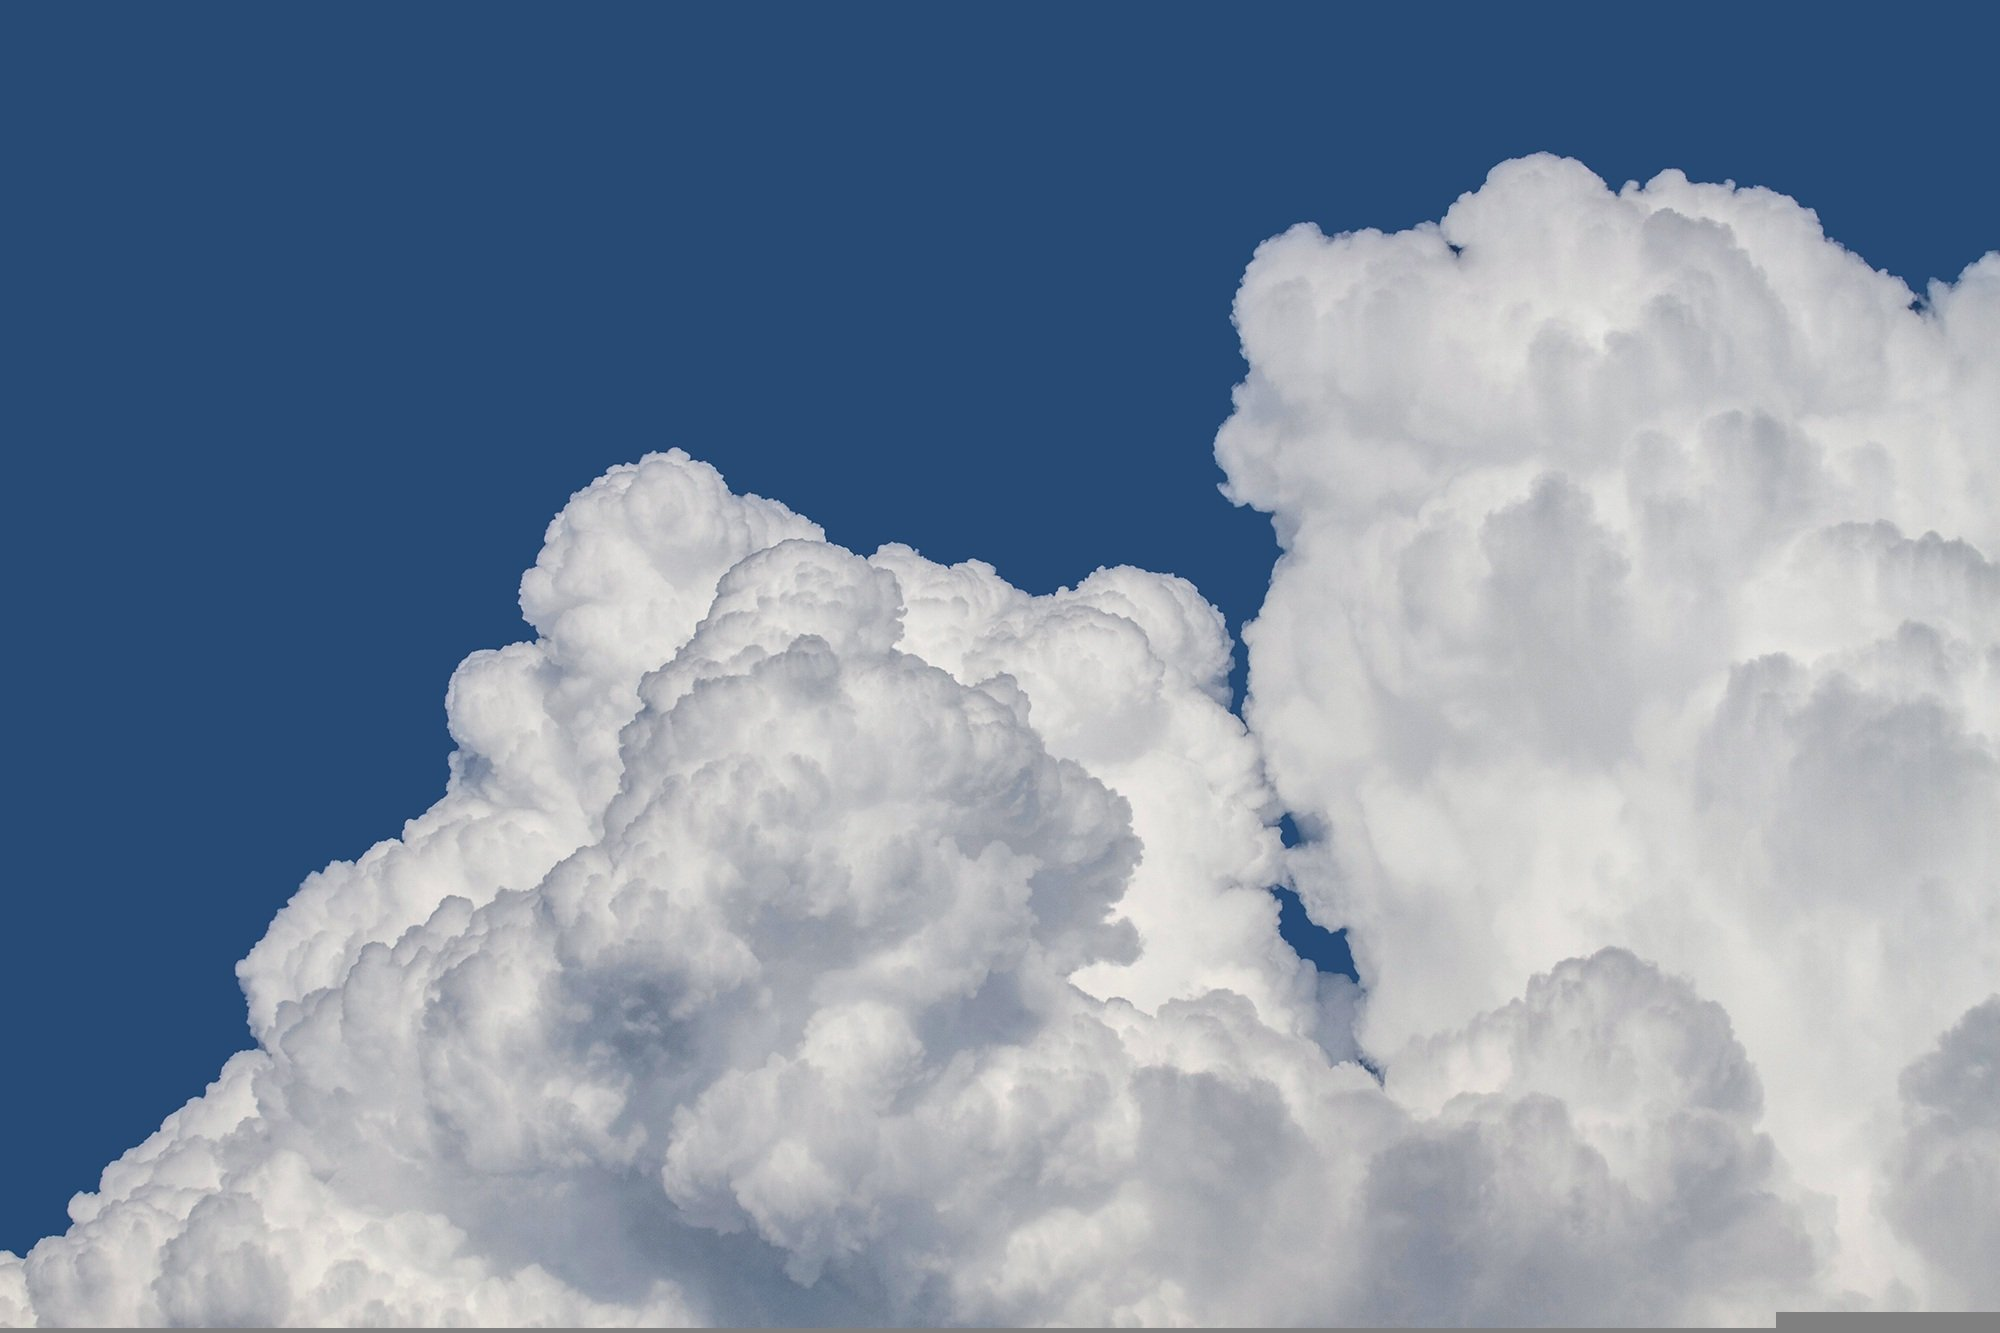
\includegraphics[width=\paperwidth,height=\paperheight]{image/nuage}
        };
    \end{tikzpicture}
}


\chapter{Perspectives pour la suite}
\label{chap:perspectives}

\section{Cap visé : passage vers la business layer}

La perspective centrale de la suite de parcours est un déplacement progressif vers la \textit{business layer}\footnote{Par \textit{business layer}, j'entends la couche de pilotage orientée valeur : cadrage stratégique, priorisation, arbitrages de portefeuille et alignement des parties prenantes.}, sans rupture avec le socle technique construit jusqu'ici. L'enjeu n'est pas d'abandonner la dimension d'ingénierie, mais de l'articuler à des responsabilités de pilotage : cadrage de valeur, arbitrage de priorités, alignement des parties prenantes et structuration de trajectoires produit.

Cette orientation s'appuie sur une conviction opérationnelle : la crédibilité business est plus solide lorsqu'elle est adossée à une compréhension réelle du produit. La capacité à décider au bon niveau de granularité dépend ici d'un double ancrage : compréhension technique des contraintes et lecture stratégique des impacts.

\section{Levier de professionnalisation : certification PRINCE2}

La certification PRINCE2, déjà obtenue, est mobilisée comme levier de transition vers ce positionnement hybride. Elle apporte un cadre de gouvernance, de gestion des risques et de pilotage par étapes, directement complémentaire des acquis développés dans ce portfolio.

Le bénéfice attendu est double :
\begin{itemize}
  \item renforcer la capacité à dialoguer avec des décideurs non techniques sur des bases structurées ;
  \item conserver un avantage différenciant en reliant décisions de management et faisabilité technique réelle.
\end{itemize}

Autrement dit, l'objectif n'est pas de devenir un profil de surface, mais un profil de jonction capable d'assurer l'intelligence entre stratégie et exécution.

\section{Avantage concurrentiel visé}

Dans des environnements où les discours de transformation sont nombreux, l'avantage recherché est la cohérence entre parole, méthode et réalisation. La valeur professionnelle visée repose sur une posture claire : ne pas uniquement "vendre" une vision, mais contribuer à la construire de manière traçable, testable et utile pour l'organisation.

Cette posture hybride vise à réduire un écart fréquent dans les projets complexes : d'un côté les profils très orientés pilotage sans profondeur technique, de l'autre les profils très techniques sans lisibilité stratégique. La trajectoire retenue cherche à tenir ensemble ces deux exigences, afin de conserver une parole crédible devant les décideurs et une action pertinente au contact du produit.

\section{Conclusion}

Ce portfolio documente une progression qui dépasse l'acquisition d'outils isolés. Il montre une évolution de posture : passer d'une logique d'exécution technique à une logique d'orchestration, capable de relier besoins, décisions, preuves et résultats.

La suite prolonge cette dynamique. Le passage vers la business layer, soutenu par la certification PRINCE2 déjà effectuée et par l'ancrage technique conservé, constitue la prochaine strate de développement.

Cette certification constitue aussi une preuve concrète pour de futurs employeurs : elle atteste que je dispose des compétences nécessaires en gouvernance, en structuration et en pilotage pour réussir cette transition.

L'ambition n'est pas de changer de camp, mais d'augmenter la capacité d'impact : comprendre, décider, et faire aboutir avec rigueur.

\clearpage
\ClearShipoutPictureBG

% : Bibliographie ---
\newpage
\printbibliography[heading=bibintoc, title={Bibliographie}]

% : Annexes ---
\begin{appendices}
  % =============================================================================
% FICHIER PRINCIPAL DES ANNEXES
% =============================================================================
% Ce fichier coordonne toutes les annexes du portfolio.
%
% TYPES D'ANNEXES SUPPORTÉS :
%
% 1. ANNEXE LATEX (section rédigée en LaTeX) :
%    \input{annexes/nom_fichier}
%
% 2. ANNEXE PDF (document PDF externe) :
%    \annexepdf{Titre de l'annexe}{annexes/pdfs/nom_fichier.pdf}
%    Variantes :
%      \annexepdf[pages=1]{Titre (1ère page seulement)}{annexes/pdfs/fichier.pdf}
%      \annexepdf[pages=1-3]{Titre (pages 1 à 3)}{annexes/pdfs/fichier.pdf}
%      \annexepdf[pages={1,3,5}]{Titre (pages spécifiques)}{annexes/pdfs/fichier.pdf}
%
% =============================================================================

% : Annexe A : contrat d'apprentissage ---
\chapter{Contrat d'apprentissage}
\label{annex:contrat-apprentissage}
\annexefiche
  {Document contractuel signé en début d'année académique 2025--2026}
  {Master HES-SO Innokick -- engagement pédagogique initial validé avec le professeur référent}
  {Cadre initial des objectifs, compétences cibles et critères de progression (chapitre \textit{Contrat individuel d'apprentissage})}
  {Aucun caviardage (document académique officiel)}
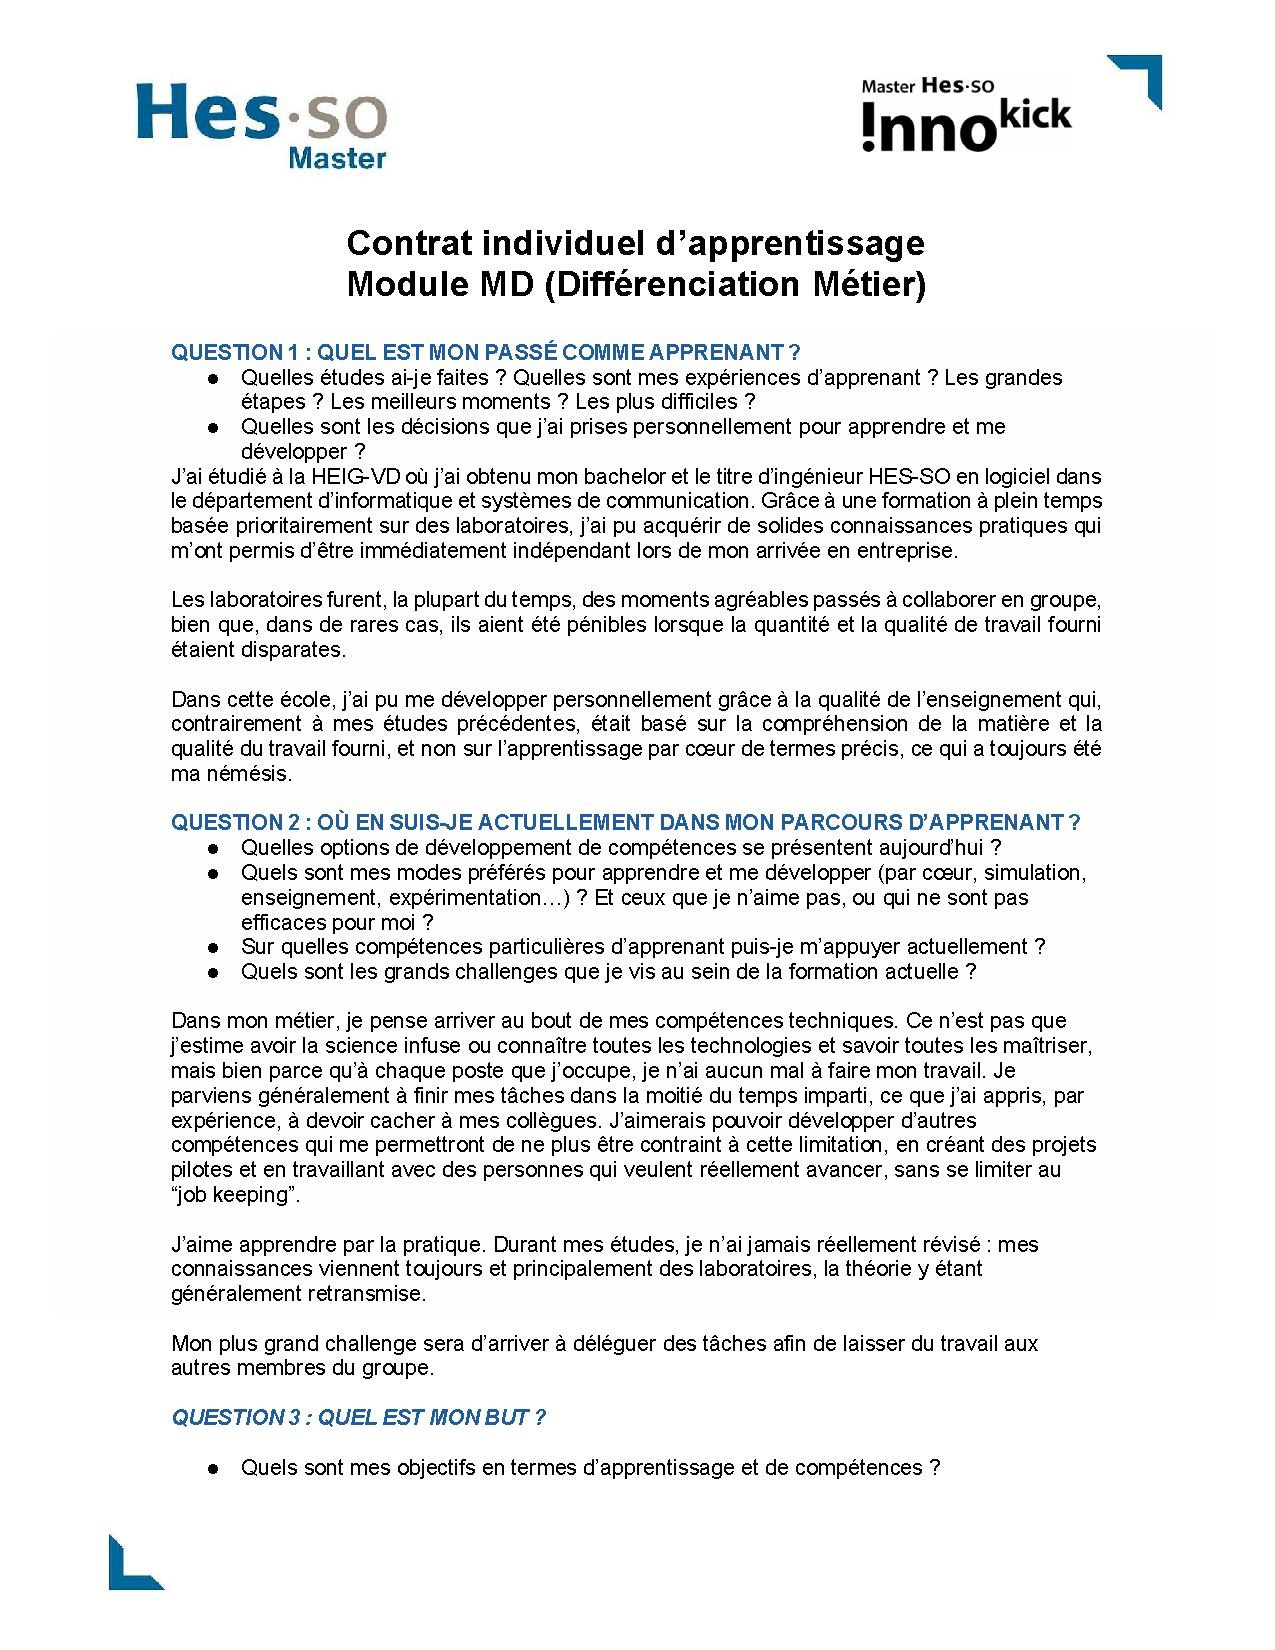
\includepdf[pages=-, pagecommand={\thispagestyle{annexepages}}]{annexes/pdfs/annexe-A-contrat-apprentissage.pdf}

% : Annexe B : Note de décision technique NDT-SW-001 ---
% =============================================================================
% ANNEX B — TECHNICAL DECISION NOTE NDT-SW-001
% =============================================================================

\chapter{Technical Decision Note: NDT-SW-001}
\label{annex:ndt-sw-001}

% --- Note de mise en contexte (portfolio) -------------------------------------
\begin{tcolorbox}[colback=blue!5, colframe=blue!40!black, boxrule=0.5pt, arc=3pt,
  left=8pt, right=8pt, top=6pt, bottom=6pt]
  \small\itshape
  \textbf{Note du portfolio.} Ce document est un artefact professionnel r\'eel,
  produit dans le cadre de la certification IEC~62304 chez TWIICE. Il a \'et\'e
  reformatt\'e en \LaTeX{} afin de pouvoir \^etre int\'egr\'e directement dans
  ce portfolio sous forme de source compilable.

  Conform\'ement aux r\`egles de confidentialit\'e de l'entreprise, les
  informations propres \`a TWIICE (noms des collaborateurs, dates internes,
  signatures) ont \'et\'e \textbf{caviard\'ees} et sont repr\'esent\'ees par
  des barres noires (\caviarder[1.2cm]). Le contenu technique et m\'ethodologique
  du document est, quant \`a lui, int\'egralement reproduit.
\end{tcolorbox}

\bigskip

% --- Document header ----------------------------------------------------------
\begin{tcolorbox}[colback=gray!8, colframe=gray!50, boxrule=0.5pt, arc=3pt,
  left=8pt, right=8pt, top=6pt, bottom=6pt]
  \begin{tabularx}{\linewidth}{@{}p{4.2cm}X@{}}
    \textbf{Reference}          & NDT-SW-001 \\[3pt]
    \textbf{Subject}            & Selection of tooling for SOUP and software artefact traceability \\[3pt]
    \textbf{Applicable standard}& IEC~62304:2006+A1:2015 --- Clause~8 (Software configuration management) \\[3pt]
    \textbf{Author}             & Alexandre Gati --- Software Engineer \\[3pt]
    \textbf{Date}               & \caviarder[2.5cm] \\[3pt]
    \textbf{Status}             & \textbf{Under Review} \\
  \end{tabularx}
\end{tcolorbox}

\bigskip

% ==============================================================================
\section*{1.\quad Context and problem statement}
% ==============================================================================

The TWIICE software team develops the embedded software for a class~IIa medical exoskeleton (MDR Regulation 2017/745). This software incorporates several third-party components (SOUP --- \textit{Software of Unknown Provenance}) whose management is governed by the IEC~62304 standard.

Clause~8 of IEC~62304 mandates a software configuration management system that ensures:

\begin{itemize}
  \item \textbf{Unique identification} of every configuration item (source code, SOUP, build artefacts, documents);
  \item \textbf{Change control} with full traceability;
  \item \textbf{Reproducibility} of any released version of the software;
  \item \textbf{End-to-end traceability}: requirement $\rightarrow$ specification $\rightarrow$ code $\rightarrow$ test $\rightarrow$ release.
\end{itemize}

The team lacked a formalised system meeting these requirements. Several parallel technical debates (processor selection, communication architecture, DevOps tooling) were dispersing collective energy. An Eisenhower matrix prioritisation (cf. Phase~2, Espace modules chapter, in this portfolio) identified SOUP traceability as the \textbf{urgent and important} issue, directly blocking certification.

% ==============================================================================
\section*{2.\quad Options evaluated}
% ==============================================================================

Three options were analysed using a multi-criteria build-vs-buy framework.

\paragraph{Option A --- GitLab (cloud)}
Use of the existing GitLab instance for source code versioning, extended to package registries (GitLab Container Registry, Package Registry) and CI/CD pipelines for automated builds and tests.

\begin{itemize}
  \item \textit{Main advantage}: tool already mastered by the team, marginal cost (included in the existing subscription), immediate deployment.
  \item \textit{Main limitation}: cloud hosting requires a cybersecurity compliance analysis for a medical device.
\end{itemize}

\paragraph{Option B --- Custom solution (in-house development)}
Design and development of a bespoke storage and versioning system, hosted on-premises.

\begin{itemize}
  \item \textit{Main advantage}: full control over format, hosting and security.
  \item \textit{Main limitation}: high development cost (estimate: several person-weeks), ongoing maintenance burden, timeline incompatible with the certification schedule.
\end{itemize}

\paragraph{Option C --- JFrog Artifactory}
Dedicated package manager specialised in binary artefact storage with metadata, checksums and CI/CD integration.

\begin{itemize}
  \item \textit{Main advantage}: native artefact traceability and integrity features.
  \item \textit{Main limitation}: additional licence required, high vendor dependency (proprietary solution).
\end{itemize}

% ==============================================================================
\section*{3.\quad Decision criteria}
% ==============================================================================

The options were assessed against six criteria defined collectively by the software team and the quality team.

\begin{table}[h!]
  \centering\small
  \begin{tabularx}{\textwidth}{|p{3.2cm}|p{2cm}|X|X|X|}
    \hline
    \textbf{Criterion} & \textbf{Weight} & \textbf{GitLab (cloud)} & \textbf{Custom solution} & \textbf{JFrog Artifactory} \\
    \hline
    Integration complexity & High     & \ok{Low}       & \nok{High}          & \warn{Medium} \\
    \hline
    Cost (licence + hours) & High     & \ok{Included}  & \nok{High}          & \warn{Extra licence} \\
    \hline
    IEC~62304 traceability & Critical & \ok{Good}      & \ok{Full}           & \ok{Good} \\
    \hline
    Implementation lead time & High   & \ok{Immediate} & \nok{Weeks/months}  & \ok{A few days} \\
    \hline
    Vendor dependency      & Medium   & \warn{Medium}  & \ok{None}           & \nok{High} \\
    \hline
    Cybersecurity risk     & High     & \warn{Moderate (cloud)} & \ok{Low (on-prem)} & \warn{Moderate (self-hosted possible)} \\
    \hline
  \end{tabularx}
  \caption{Multi-criteria grid --- IEC~62304 configuration management options}
  \label{tab:ndt-criteres}
\end{table}

% ==============================================================================
\section*{4.\quad Analysis and recommendation}
% ==============================================================================

\textbf{Option A (GitLab cloud)} offers the best overall balance:

\begin{itemize}
  \item \textbf{Lead time}: immediate deployment, compatible with the certification schedule.
  \item \textbf{Cost}: zero additional cost (existing subscription).
  \item \textbf{Skills}: tool already mastered by the team, no learning curve.
  \item \textbf{Traceability}: native versioning (tags, releases), package registries, CI/CD pipeline automating tests and builds.
\end{itemize}

Option B (custom) was rejected despite offering full control, due to a timeline and cost incompatible with the resources of a startup in certification phase.

Option C (JFrog) was rejected due to high vendor dependency and additional licence cost, offering marginal functional gain over GitLab in this context.

% ==============================================================================
\section*{5.\quad Selected decision}
% ==============================================================================

\begin{decisionbox}
\textbf{Option A --- GitLab (cloud)}

Use of the existing GitLab instance as the primary software configuration management system, including:

\begin{itemize}
  \item Source code versioning (Git);
  \item Package and build artefact registry (GitLab Package Registry);
  \item CI/CD pipeline for automated unit, integration and artefact generation;
  \item Tags and releases for unique identification of each delivered version.
\end{itemize}
\end{decisionbox}

% ==============================================================================
\section*{6.\quad Residual risks and mitigation measures}
% ==============================================================================

\begin{table}[h!]
  \centering\small
  \begin{tabularx}{\textwidth}{|X|p{2cm}|p{1.8cm}|X|}
    \hline
    \textbf{Risk} & \textbf{Likelihood} & \textbf{Impact} & \textbf{Mitigation} \\
    \hline
    Cloud hosting --- cybersecurity compliance for a medical device
      & Medium & High
      & Vendor compliance analysis (SOC~2, ISO~27001 certifications). Evaluate migration to GitLab self-hosted if required by audit. \\
    \hline
    Vendor dependency --- pricing or terms-of-service change
      & Low & Medium
      & Data exportable (native Git). Migration plan to an alternative (Gitea, GitLab self-hosted) documented. \\
    \hline
    Incomplete traceability --- gap between IEC~62304 requirements and native features
      & Low & High
      & Supplemented by manual documentation (SOUP list, requirements-code-tests traceability matrix). Integrated into the \textit{Definition of Done}. \\
    \hline
    Cloud service availability --- outage impacting development
      & Low & Low
      & Local Git clones on every workstation. Periodic backups of the package registry. \\
    \hline
  \end{tabularx}
  \caption{Residual risks and mitigation measures --- NDT-SW-001}
  \label{tab:ndt-risques}
\end{table}

% ==============================================================================
\section*{8.\quad Approval}
% ==============================================================================

\begin{table}[h!]
  \centering
  \begin{tabular}{|p{4cm}|p{3.5cm}|p{2.5cm}|p{3cm}|}
    \hline
    \textbf{Role} & \textbf{Name} & \textbf{Date} & \textbf{Signature} \\
    \hline
    Author (Software Eng.) & Alexandre Gati     & \caviarder[2cm] & \caviarder[2.5cm] \\[6pt]
    \hline
    Software Architect     & \caviarder[2.5cm]  & \caviarder[2cm] & \caviarder[2.5cm] \\[6pt]
    \hline
    Quality Manager        & \caviarder[2.5cm]  & \caviarder[2cm] & \caviarder[2.5cm] \\[6pt]
    \hline
  \end{tabular}
  \caption{Approval table --- NDT-SW-001}
  \label{tab:ndt-approbation}
\end{table}




% : Annexe C : Extrait du backlog priorisé ---
% =============================================================================
% ANNEX C — PRIORITISED BACKLOG EXTRACT
% =============================================================================

\chapter{Prioritised Backlog Extract}
\label{annex:backlog}

% --- Note de mise en contexte (portfolio) -------------------------------------
\begin{tcolorbox}[colback=blue!5, colframe=blue!40!black, boxrule=0.5pt, arc=3pt,
  left=8pt, right=8pt, top=6pt, bottom=6pt]
  \small\itshape
  \textbf{Note du portfolio.} Ce document est un extrait du backlog de
  l'\'equipe logicielle TWIICE, export\'e depuis le board GitLab du projet.
  Il illustre la hi\'erarchisation des t\^aches apr\`es application de la
  matrice d'Eisenhower (cf. Phase~2, Espace modules du pr\'esent portfolio).

  Conform\'ement aux r\`egles de confidentialit\'e de l'entreprise, les
  informations sensibles (num\'eros d'issues, noms des collaborateurs, dates,
  jalons internes) ont \'et\'e \textbf{caviard\'ees} et sont repr\'esent\'ees
  par des barres noires (\caviarder[1.2cm]). Les intitul\'es des t\^aches et
  leur description technique sont, quant \`a eux, int\'egralement reproduits.
\end{tcolorbox}

\bigskip

% --- Sprint / Project header --------------------------------------------------
\begin{tcolorbox}[colback=gray!8, colframe=gray!50, boxrule=0.5pt, arc=3pt,
  left=8pt, right=8pt, top=6pt, bottom=6pt]
  \begin{tabularx}{\linewidth}{@{}p{4cm}X@{}}
    \textbf{Project}   & TWIICE Exoskeleton --- Software \\[3pt]
    \textbf{Milestone} & \caviarder[3cm] \\[3pt]
    \textbf{Sprint}    & \caviarder[2cm]\quad
                         (\caviarder[2cm]\;--\;\caviarder[2cm]) \\[3pt]
    \textbf{Board}     & \caviarder[5cm] \\[3pt]
    \textbf{Exported by} & Alexandre Gati \\[3pt]
    \textbf{Export date} & \caviarder[2.5cm] \\
  \end{tabularx}
\end{tcolorbox}

\bigskip

% ==============================================================================
\section*{Context}
% ==============================================================================

The following extract lists the software issues identified and re-prioritised
following an Eisenhower matrix exercise conducted with the team (see Annex~B,
\S1). Issues are grouped by priority level --- \highprio, \mediumprio,
\lowprio{} --- and ordered within each group by creation date. Redacted fields
(\caviarder[0.9cm]) contain information covered by the company's
confidentiality policy.

\bigskip

% ==============================================================================
% BACKLOG TABLE
% ==============================================================================

\begingroup
\setlength{\tabcolsep}{3pt}
\begin{table}[h!]
  \centering\footnotesize
  \begin{tabularx}{\textwidth}{|p{1.4cm}|p{1.1cm}|X|p{2.0cm}|p{1.4cm}|p{1.7cm}|}
    \hline
    \rowcolor{gray!15}
    \textbf{Priority} & \textbf{Issue\,\#} & \textbf{Title \& description} &
    \textbf{Assignee} & \textbf{Due} & \textbf{Status} \\
    \hline

    % ------------------------------------------------------------------
    % HIGH PRIORITY
    % ------------------------------------------------------------------

    \highprio
      & \caviarder[0.8cm]
      & \textbf{Set up SOUP traceability --- GitLab Package Registry}
        \newline{\footnotesize
          Register all third-party libraries (SOUP list) in the GitLab Package
          Registry. Ensure each entry includes version, licence, source URL and
          checksum, per IEC~62304 \S8.1.2.
          \newline\textit{Labels:} \texttt{iec-62304}, \texttt{certification},
          \texttt{sprint-\caviarder[0.4cm]}}
      & \caviarder[2.2cm]
      & \caviarder[1.5cm]
      & \sinprogress \\
    \hline

    \highprio
      & \caviarder[0.8cm]
      & \textbf{Document all third-party components (IEC~62304 \S8)}
        \newline{\footnotesize
          Produce the SOUP list artefact required by IEC~62304 clause~8:
          component name, version, publisher, risk classification.
          Cross-reference with the software requirements specification.
          \newline\textit{Labels:} \texttt{iec-62304}, \texttt{documentation},
          \texttt{sprint-\caviarder[0.4cm]}}
      & \caviarder[2.2cm]
      & \caviarder[1.5cm]
      & \sinprogress \\
    \hline

    \highprio
      & \caviarder[0.8cm]
      & \textbf{Define CI/CD pipeline --- automated build \& test artefacts}
        \newline{\footnotesize
          Configure the GitLab CI pipeline to produce reproducible build
          artefacts (binary, SBOM, test report) and publish them to the
          Package Registry with immutable versioning tags.
          \newline\textit{Labels:} \texttt{ci-cd}, \texttt{iec-62304},
          \texttt{sprint-\caviarder[0.4cm]}}
      & \caviarder[2.2cm]
      & \caviarder[1.5cm]
      & \stodo \\
    \hline

    % ------------------------------------------------------------------
    % MEDIUM PRIORITY
    % ------------------------------------------------------------------

    \mediumprio
      & \caviarder[0.8cm]
      & \textbf{Standardise documentation templates (IEC~62304)}
        \newline{\footnotesize
          Create shared GitLab Wiki templates for: SOUP list, change request,
          software release note, design review record. Reduces manual overhead
          and ensures consistent artefact format across sprints.
          \newline\textit{Labels:} \texttt{documentation},
          \texttt{sprint-\caviarder[0.4cm]}}
      & \caviarder[2.2cm]
      & \caviarder[1.5cm]
      & \stodo \\
    \hline

    \mediumprio
      & \caviarder[0.8cm]
      & \textbf{Update SOUP risk assessment --- IEC~62304 \S7.2}
        \newline{\footnotesize
          Review existing risk assessments for embedded SOUP (FreeRTOS,
          libmodbus, \caviarder[1.5cm]). Align severity classifications with
          the updated device risk file (MDR class~IIa context).
          \newline\textit{Labels:} \texttt{risk}, \texttt{iec-62304}}
      & \caviarder[2.2cm]
      & \caviarder[1.5cm]
      & \sbacklog \\
    \hline

    % ------------------------------------------------------------------
    % LOW PRIORITY
    % ------------------------------------------------------------------

    \lowprio
      & \caviarder[0.8cm]
      & \textbf{Evaluate MCU vs Jetson for user interface module}
        \newline{\footnotesize
          Comparative benchmark: processing power, energy budget, SDK
          maturity, lead time. Decision deferred --- not blocking
          certification. To be scheduled post-milestone
          \caviarder[1.2cm].
          \newline\textit{Labels:} \texttt{hardware}, \texttt{research}}
      & \caviarder[2.2cm]
      & \caviarder[1.5cm]
      & \sbacklog \\
    \hline

    \lowprio
      & \caviarder[0.8cm]
      & \textbf{Benchmark supplementary DevOps tools}
        \newline{\footnotesize
          Evaluate JFrog Artifactory, Nexus Repository and Harbor as
          potential complements to the GitLab Package Registry. No
          blocker identified --- team comfort improvement only.
          \newline\textit{Labels:} \texttt{devops}, \texttt{tooling}}
      & \caviarder[2.2cm]
      & \caviarder[1.5cm]
      & \sbacklog \\
    \hline

  \end{tabularx}
  \caption{Prioritised backlog extract --- TWIICE Software, post-Eisenhower
    matrix triage}
  \label{tab:backlog}
\end{table}
\endgroup

% ==============================================================================
\section*{Traceability to the Eisenhower matrix}
% ==============================================================================

The table below maps each priority group to the corresponding quadrant of the
Eisenhower matrix applied during the Phase~2 (Definition) workshop.

\begin{table}[h!]
  \centering\small
  \begin{tabularx}{\textwidth}{|p{1.6cm}|p{3.5cm}|X|}
    \hline
    \textbf{Priority} & \textbf{Eisenhower quadrant} & \textbf{Rationale} \\
    \hline
    \highprio
      & Urgent \& Important
      & Directly blocks the IEC~62304 certification audit. Must be resolved
        within the current or immediately following sprint. \\
    \hline
    \mediumprio
      & Important, not urgent
      & Required for long-term compliance and team efficiency, but does not
        block the next certification milestone. Scheduled in upcoming sprints. \\
    \hline
    \lowprio
      & Not important (current context)
      & Debated actively during the workshop but identified as non-blocking.
        Deferred to the post-certification backlog. \\
    \hline
  \end{tabularx}
  \caption{Mapping between backlog priority levels and Eisenhower quadrants}
  \label{tab:backlog-eisenhower}
\end{table}







% : Annexe D : Software Development Plan (reproduction markdown caviardee) ---
% =============================================================================
% ANNEX D : SOFTWARE DEVELOPMENT PLAN (FORMALIZED AND REDACTED VERSION)
% =============================================================================

\chapter{Software Development Plan (formalized and redacted version)}
\label{annex:sdp-markdown}

\begin{tcolorbox}[colback=blue!5, colframe=blue!40!black, boxrule=0.5pt, arc=3pt,
  left=8pt, right=8pt, top=6pt, bottom=6pt]
  \small\itshape
  \textbf{Avertissement.} Le contenu ci-dessous est une reproduction formalisee en \LaTeX{} du Software Development Plan original. Cette version a ete volontairement \textbf{tronquee} et caviardee afin de proteger les informations sensibles (identites, identifiants documentaires internes, liens, details d'infrastructure et metadonnees de pilotage). Des notes de bas de page explicatives ont egalement ete ajoutees pour en faciliter la lecture par un public \textbf{novice}.
\end{tcolorbox}

\section*{1. Document control}

\subsection*{1.1 Roles}
\begin{tabularx}{\textwidth}{|p{3.3cm}|p{2.5cm}|X|p{3cm}|}
\hline
\textbf{Role} & \textbf{Name} & \textbf{Reason for signature} & \textbf{Signature \& date} \\
\hline
System Quality Manager & \caviarder[2.8cm] & Document Owner, Author & \caviarder[2.8cm] \\
\hline
Software Engineer & \caviarder[2.8cm] & Reviewer & \caviarder[2.8cm] \\
\hline
Software Manager & \caviarder[2.8cm] & Approver & \caviarder[2.8cm] \\
\hline
\end{tabularx}

\subsection*{1.2 Version history}
\begin{tabularx}{\textwidth}{|p{2.5cm}|X|}
\hline
\textbf{Version} & \textbf{Description} \\
\hline
1 & Initial version \\
\hline
\end{tabularx}

\subsection*{1.3 References (redacted)}
\begin{longtable}{|p{1.4cm}|p{12cm}|}
\hline
\textbf{Ref.} & \textbf{Document} \\
\hline
R1 & Internal controlled procedure (\caviarder[5.2cm]) \\
\hline
R2 & Internal controlled procedure (\caviarder[5.2cm]) \\
\hline
R3 & Internal controlled procedure (\caviarder[5.2cm]) \\
\hline
R4 & Internal controlled procedure (\caviarder[5.2cm]) \\
\hline
R5 & IEC~62304:2006+AMD1:2015, Medical device software life cycle processes \\
\hline
R6 & Internal controlled procedure (\caviarder[5.2cm]) \\
\hline
R7 & Internal controlled procedure (\caviarder[5.2cm]) \\
\hline
R8 & Internal controlled procedure (\caviarder[5.2cm]) \\
\hline
R9 & Internal controlled procedure (\caviarder[5.2cm]) \\
\hline
R10 & Internal controlled procedure (\caviarder[5.2cm]) \\
\hline
R11 & FDA: Content of Premarket Submissions for Device Software Functions \\
\hline
R12-R19 & Internal project documents (plans, architecture, risk records, detailed design): \caviarder[3.4cm] \\
\hline
\end{longtable}

\subsection*{1.4 Definitions (extract)}
\begin{longtable}{|p{3cm}|p{10.4cm}|}
\hline
\textbf{Term} & \textbf{Definition} \\
\hline
Software System & Integrated collection of Software Items organized to accomplish a function set (IEC~62304 3.28). \\
\hline
Software Item & Any identifiable part of a computer program (IEC~62304 3.25). \\
\hline
Software Unit & Software Item not subdivided into other items (IEC~62304 3.29). \\
\hline
SOUP / OTS & Third-party software not fully controlled through manufacturer life cycle. \\
\hline
SDP & Software Development Plan. \\
\hline
SRS & Software Requirements Specification: defines what software shall do. \\
\hline
SDDD & Software Detailed Design Document: internal design of software items/units. \\
\hline
Software Anomaly & Condition deviating from expected behavior. \\
\hline
\end{longtable}

\section*{2. Purpose and scope}

The SDP defines software development processes for the medical device in compliance with IEC~62304 and internal controlled procedures (\caviarder[2.8cm]).

\subsection*{2.1 Scope}
The plan covers software components in scope: \caviarder[5.5cm].

The document is reviewed at each Gate Review (G1 to G4) and updated under formal change control.

\section*{3. Software safety classification}

\textbf{Preliminary classification:} \caviarder[2.2cm] (conservative assumption for an active medical device).

\textbf{Segregation strategy:}
\begin{itemize}
  \item Critical control loops handled as \caviarder[1.8cm].
  \item Auxiliary applications potentially classified as \caviarder[2.4cm] if architectural segregation is demonstrated.
\end{itemize}

\section*{4. Roles and responsibilities (extrait)}

\begin{tabularx}{\textwidth}{|p{3cm}|X|p{3cm}|}
\hline
\textbf{Role} & \textbf{Responsibilities} & \textbf{Assigned to} \\
\hline
Software Lead & Executes the SDP, arbitrates architecture, and coordinates verification and change impacts. & \caviarder[2.8cm] \\
\hline
Software Developer & Development, unit testing, static analysis, and merge requests. & \caviarder[2.8cm] \\
\hline
Configuration Manager & SCM, CI/CD pipelines, SOUP management, and release baselines. & \caviarder[2.8cm] \\
\hline
Quality Manager & Traceability review, gate validation, and SOP compliance. & \caviarder[2.8cm] \\
\hline
Risk Manager & RMF follow-up\footnote{\textbf{RMF} stands for \textit{Risk Management File}. It contains the records documenting risk analysis, risk control measures, and their verification evidence.}, and safety-impact review of anomalies and changes. & \caviarder[2.8cm] \\
\hline
\end{tabularx}

\section*{5. Development life cycle model}

The project follows a V-Model integrated into the Stage-Gate process.

\begin{tabularx}{\textwidth}{|p{1.2cm}|p{2.2cm}|p{2.5cm}|X|}
\hline
\textbf{Gate} & \textbf{Phase} & \textbf{IEC~62304} & \textbf{Key software activities} \\
\hline
G0 & Planning & 5.1 & User need definition (\caviarder[2.8cm]) \\
\hline
G1 & Input \& Arch. & 5.1, 5.2, 5.3 & SDP, SRS\footnote{\textbf{SRS} stands for \textit{Software Requirements Specification}. This document formalizes verifiable software requirements.}, \caviarder[3.8cm] \\
\hline
G2 & Detailed design & 5.4, 5.5 & SDDD\footnote{\textbf{SDDD} stands for \textit{Software Detailed Design Document}. It decomposes architecture into implementable and testable components/units.}, \caviarder[4.6cm] \\
\hline
G3 & Verification & 5.6, 5.7 & Integration, system testing, \caviarder[2.8cm] \\
\hline
G4 & Validation & 5.8 & Software release and \caviarder[2.4cm] \\
\hline
\end{tabularx}

\medskip
\textbf{Planned deviation:} SDP produced at G1 (instead of G0), since \caviarder[5.8cm].

\section*{6. Traceability and verification framework}

\textbf{Traceability rules:}
\begin{itemize}
  \item Each software requirement has an upstream link to a system requirement and/or risk control measure.
  \item Each software requirement has downstream links to design, code, and verification activity.
  \item Completeness review is performed before each gate.
\end{itemize}

\textbf{Verification strategy (summary):}
\begin{tabularx}{\textwidth}{|p{1.2cm}|p{3.1cm}|X|}
\hline
\textbf{Gate} & \textbf{Verification activity} & \textbf{Acceptance criteria} \\
\hline
G1 & Design review & Requirements and architecture are baselined; \caviarder[3.6cm] \\
\hline
G2 & Unit verification & Static analysis compliant, \caviarder[3.8cm] \\
\hline
G3 & Integration \& system verification & Requirement coverage and integration/system tests validated, \caviarder[2.8cm] \\
\hline
G4 & Release verification & Release package complete; \caviarder[3.4cm] \\
\hline
\end{tabularx}

\section*{7. Software configuration management (SCM)}

SCM is aligned with internal controlled procedures (\caviarder[2.2cm]) using a controlled branching strategy.

\begin{itemize}
  \item \caviarder[2.6cm]: release baseline, direct commits prohibited.
  \item \caviarder[2.6cm]: continuous integration of evolutions.
  \item \caviarder[2.6cm]: preparation of official versions.
  \item \caviarder[2.6cm]: post-release correction with impact analysis.
  \item \caviarder[3.8cm]: development branches.
\end{itemize}

\section*{8. SOUP, cybersecurity, release and maintenance}

\textbf{SOUP management:}
\begin{itemize}
  \item SOUP inventory maintained and periodically reviewed.
  \item SOUP components verified through test plans.
  \item Vulnerability and end-of-life monitoring performed continuously.
\end{itemize}

\textbf{Release:}
release includes version, hash, residual anomalies, SOUP components, and \caviarder[3.8cm], followed by controlled archiving.

\textbf{Problem resolution and maintenance:}
each anomaly follows a documented cycle: logging, triage, investigation, resolution, regression check, then traceability to \caviarder[3.2cm].

\section*{9. Deliverables matrix (redacted summary)}

\begin{tabularx}{\textwidth}{|X|p{2.4cm}|p{1.5cm}|p{2.1cm}|}
\hline
\textbf{Deliverable} & \textbf{Format} & \textbf{Gate} & \textbf{IEC~62304} \\
\hline
SDP & \caviarder[2.2cm] signed & G1 & 5.1 \\
\hline
SRS / Architecture & \caviarder[2.2cm] signed & G1 & 5.2 / 5.3 \\
\hline
SDDD + unit evidence & \caviarder[3.2cm] + PDF signed & G2 & 5.4 / 5.5 \\
\hline
Integration/System tests + traceability matrix & \caviarder[2.6cm] & G3 & 5.6 / 5.7 \\
\hline
Release notes + final SOUP list + software RMF section & \caviarder[2.6cm] & G4 & 5.8 / clause 7 \\
\hline
\end{tabularx}

\medskip
\noindent\textit{Note: detailed document identifiers, storage links, internal audit trails, and operational references are redacted in this portfolio version.}





% : Annexe E : Journal réflexif ---
\chapter{Journal réflexif : Master Innokick}
\label{annex:journal-reflexif}
\annexefiche
  {Entrées produites au fil de l'année académique 2025--2026}
  {Journal personnel de suivi des apprentissages (cours, situations, prises de recul)}
  {Fond réflexif transversal mobilisé dans les analyses A2/B4/C2 et dans le chapitre \textit{Perspectives}}
  {Caviardage léger : éventuelles données sensibles personnelles ou tierces}
\includepdf[pages=-, pagecommand={\thispagestyle{annexepages}}]{annexes/pdfs/annexe-E-journal-reflexif.pdf}

% : Annexe F : Compte-rendu de la première rétrospective (B4) ---
% =============================================================================
% ANNEX F : TEAM RETROSPECTIVE REPORT (B4), REDACTED
% =============================================================================

\chapter{First team retrospective report (B4)}
\label{annex:retro-b4}

\begin{tcolorbox}[colback=blue!5, colframe=blue!40!black, boxrule=0.5pt, arc=3pt,
  left=8pt, right=8pt, top=6pt, bottom=6pt]
  \small\itshape
  \textbf{Avertissement.} Cette annexe est une reproduction \textbf{non fidele} d'un compte-rendu de retrospective utilise en contexte professionnel. Elle est volontairement adaptee, tronquee et caviardee a des fins de \textbf{demonstration} et de \textbf{preuve} dans le portfolio. Les informations sensibles (identites, dates exactes, identifiants, references internes et metadonnees d'outillage) ont ete masquees.
\end{tcolorbox}

\bigskip

\begin{tcolorbox}[colback=gray!8, colframe=gray!50, boxrule=0.5pt, arc=3pt,
  left=8pt, right=8pt, top=6pt, bottom=6pt]
\begin{tabularx}{\linewidth}{@{}p{4.3cm}X@{}}
\textbf{Team} & TWIICE software team \\
\textbf{Related sprint} & Sprint \caviarder[1.8cm] (2 weeks) \\
\textbf{Retrospective date} & \caviarder[2.2cm] \\
\textbf{Facilitator} & \caviarder[2.6cm] \\
\textbf{Participants} & \caviarder[6cm] \\
\textbf{Context} & First complete retrospective after deployment of an IEC~62304-adapted agile framework \\
\end{tabularx}
\end{tcolorbox}

\section*{1. Retrospective objective}

Evaluate the sprint across three axes: what should continue, what should stop, and what should start in the next sprint. The operational goal is to improve agile delivery pace while strengthening certification-grade documentation quality.

\section*{2. Method applied}

The session follows a Start/Stop/Continue format, with timeboxing, collective priority voting, and final action validation. Each retained action is assigned an owner, a deadline, and a verification criterion.

\section*{3. Start / Stop / Continue results}

\begin{tabularx}{\textwidth}{|p{2.2cm}|X|}
\hline
\textbf{Continue} &
\begin{itemize}
  \item Maintain the 15-minute daily ritual focused on technical blockers and compliance risks.
  \item Keep the value $\times$ certification-risk prioritization model in the backlog.
  \item Continue cross-review between development and quality before sprint closure.
\end{itemize} \\
\hline
\textbf{Stop} &
\begin{itemize}
  \item Stop late end-of-sprint merges without complete documentation checks.
  \item Stop ambiguous tickets without explicit acceptance criteria.
  \item Stop ad hoc anomaly handling outside the prioritized queue.
\end{itemize} \\
\hline
\textbf{Start} &
\begin{itemize}
  \item Start a single DoD checklist (code, tests, IEC~62304 docs, quality review).
  \item Start a standardized "residual risks" section in each decision note.
  \item Start weekly monitoring of traceability gaps (requirements $\rightarrow$ tests $\rightarrow$ evidence).
\end{itemize} \\
\hline
\end{tabularx}

\section*{4. Retained actions and execution evidence}

\begin{tabularx}{\textwidth}{|p{4.6cm}|p{2.7cm}|p{2.4cm}|X|}
\hline
\textbf{Action} & \textbf{Owner} & \textbf{Deadline} & \textbf{Verification criterion} \\
\hline
Common DoD checklist activated on all tickets in the next sprint & \caviarder[2.1cm] & \caviarder[1.8cm] & 100\% of "Done" tickets include code + tests + documented traceability \\
\hline
"Residual risks" template added to decision notes & \caviarder[2.1cm] & \caviarder[1.8cm] & Each new decision note includes risks + mitigation section \\
\hline
Weekly traceability review institutionalized & \caviarder[2.1cm] & \caviarder[1.8cm] & Gap dashboard maintained; critical gaps closed before gate review \\
\hline
\end{tabularx}

\section*{5. How this evidence demonstrates training impact}

This retrospective evidences a change in maturity level.

\begin{itemize}
  \item \textbf{Before training}: verbal feedback loops, weak traceability, and limited action follow-through.
  \item \textbf{After training}: explicit improvement loop (observation $\rightarrow$ action $\rightarrow$ verification) with auditable artifacts.
\end{itemize}

The observable benefit is twofold: team dynamics become more stable (fewer repeated debates), and compliance becomes integrated into daily steering rather than appended at end of cycle.

\section*{6. Closure status}

\begin{tabularx}{\textwidth}{|p{4.2cm}|X|}
\hline
\textbf{Team validation} & Retrospective approved by the project team (redacted trace) \\
\hline
\textbf{Documentation trace} & Record linked to sprint artifacts \caviarder[2.0cm] and to gate preparation \caviarder[1.6cm] \\
\hline
\textbf{Link to B4 competency} & Evidence of genuine iterative adaptation in a regulated environment \\
\hline
\end{tabularx}




% : Annexe G : Package de priorisation C2 ---
% =============================================================================
% ANNEX G : C2 PRIORITIZATION PACKAGE (MATRIX + WORKSHOP + ROADMAP)
% =============================================================================

\chapter{C2 package: prioritization, workshop, and roadmap}
\label{annex:c2-priorisation}

\begin{tcolorbox}[colback=blue!5, colframe=blue!40!black, boxrule=0.5pt, arc=3pt,
  left=8pt, right=8pt, top=6pt, bottom=6pt]
  \small\itshape
  \textbf{Avertissement.} Cette annexe est une reproduction \textbf{non fidele} d'artefacts de synthese mobilises pour la competence C2. Elle est volontairement adaptee, tronquee et caviardee a des fins de \textbf{demonstration} et de \textbf{preuve} dans le portfolio. Les informations sensibles (identites, identifiants internes, references d'outillage et metadonnees projet) ont ete masquees.
\end{tcolorbox}

\section*{1. Prioritization matrix for evolutions}

\begin{tabularx}{\textwidth}{|p{3.1cm}|X|X|}
\hline
 & \textbf{High feasibility} & \textbf{Low/medium feasibility} \\
\hline
\textbf{High user impact}
&
\begin{itemize}
  \item Assisted-walking mode stability (Must)
  \item Sensor calibration reliability (Must)
\end{itemize}
&
\begin{itemize}
  \item Telemetry pipeline redesign \caviarder[1.8cm] (Should)
\end{itemize} \\
\hline
\textbf{Medium user impact}
&
\begin{itemize}
  \item Coach screen UX optimization (Should)
\end{itemize}
&
\begin{itemize}
  \item Architecture evolution \caviarder[1.8cm] (Could)
\end{itemize} \\
\hline
\textbf{Low user impact}
&
\begin{itemize}
  \item Cosmetic interface adjustments (Could)
\end{itemize}
&
\begin{itemize}
  \item Exploratory work outside sprint scope (Won't now)
\end{itemize} \\
\hline
\end{tabularx}

\medskip
\noindent\textbf{Result.} The matrix reduced a portfolio of approximately 150 requests to a prioritized core of \caviarder[1.1cm] action streams validated in workshop.

\section*{2. Workshop report: problem-definition convergence}

\begin{tcolorbox}[colback=gray!8, colframe=gray!50, boxrule=0.5pt, arc=3pt,
  left=8pt, right=8pt, top=6pt, bottom=6pt]
\begin{tabularx}{\linewidth}{@{}p{4.3cm}X@{}}
\textbf{Date} & \caviarder[2.3cm] \\
\textbf{Participants} & Software team, quality team, usage representatives \caviarder[2.2cm] \\
\textbf{Facilitator} & \caviarder[2.6cm] \\
\textbf{Objective} & Move from raw requests to 3--5 prioritized and actionable problem statements \\
\end{tabularx}
\end{tcolorbox}

\textbf{Problem statement 1 (high priority).}
Secure reliability of critical functions before extending secondary features.

\textbf{Problem statement 2 (high priority).}
Reduce lead time for blocking-anomaly handling by clarifying ownership and prioritization criteria.

\textbf{Problem statement 3 (medium priority).}
Improve readability of technical decisions to reduce cross-team debate reopenings.

\medskip
\noindent\textbf{Convergence mechanism.} Each retained problem statement is selected through structured voting, then reformulated into a shared problem sentence validated by all attending stakeholders.

\section*{3. Roadmap derived from prioritization}

\begin{tabularx}{\textwidth}{|p{3.7cm}|p{2.3cm}|X|p{2.1cm}|}
\hline
\textbf{Axis} & \textbf{Horizon} & \textbf{Operational objective} & \textbf{Indicator} \\
\hline
Critical-function reliability & Sprint S+1 to S+2 & Close critical tickets linked to assisted-walking stability & Closure rate >= \caviarder[1.1cm] \\
\hline
Anomaly flow and prioritization & Sprint S+1 & Implement weekly triage ritual + MoSCoW ranking rule & Average triage delay <= \caviarder[1.4cm] \\
\hline
Decision traceability & Sprint S+1 to S+3 & Standardize decision note + backlog linkage + verification evidence & 100\% of major decisions traceable \\
\hline
\end{tabularx}

\section*{4. Why this annex evidences competency C2}

This annex shows a complete chain:
\begin{enumerate}
  \item raw-request collection,
  \item matrix-based synthesis,
  \item workshop convergence,
  \item translation into a measurable roadmap.
\end{enumerate}

The decisive C2 evidence is the transformation of a heterogeneous request volume into prioritized, shared, and time-steerable problem statements.




% : Annexe H : Descriptif de module Différenciation métier ---
\chapter{Descriptif de module : Différenciation métier (MDM)}
\label{annex:descriptif-mdm}
\annexefiche
  {Version institutionnelle en vigueur pendant l'année 2025--2026}
  {Document officiel HES-SO Innokick -- cadre pédagogique du module MDM}
  {Justification du périmètre d'évaluation, articulation des attendus et positionnement des preuves du portfolio}
  {Aucun caviardage (document institutionnel public)}
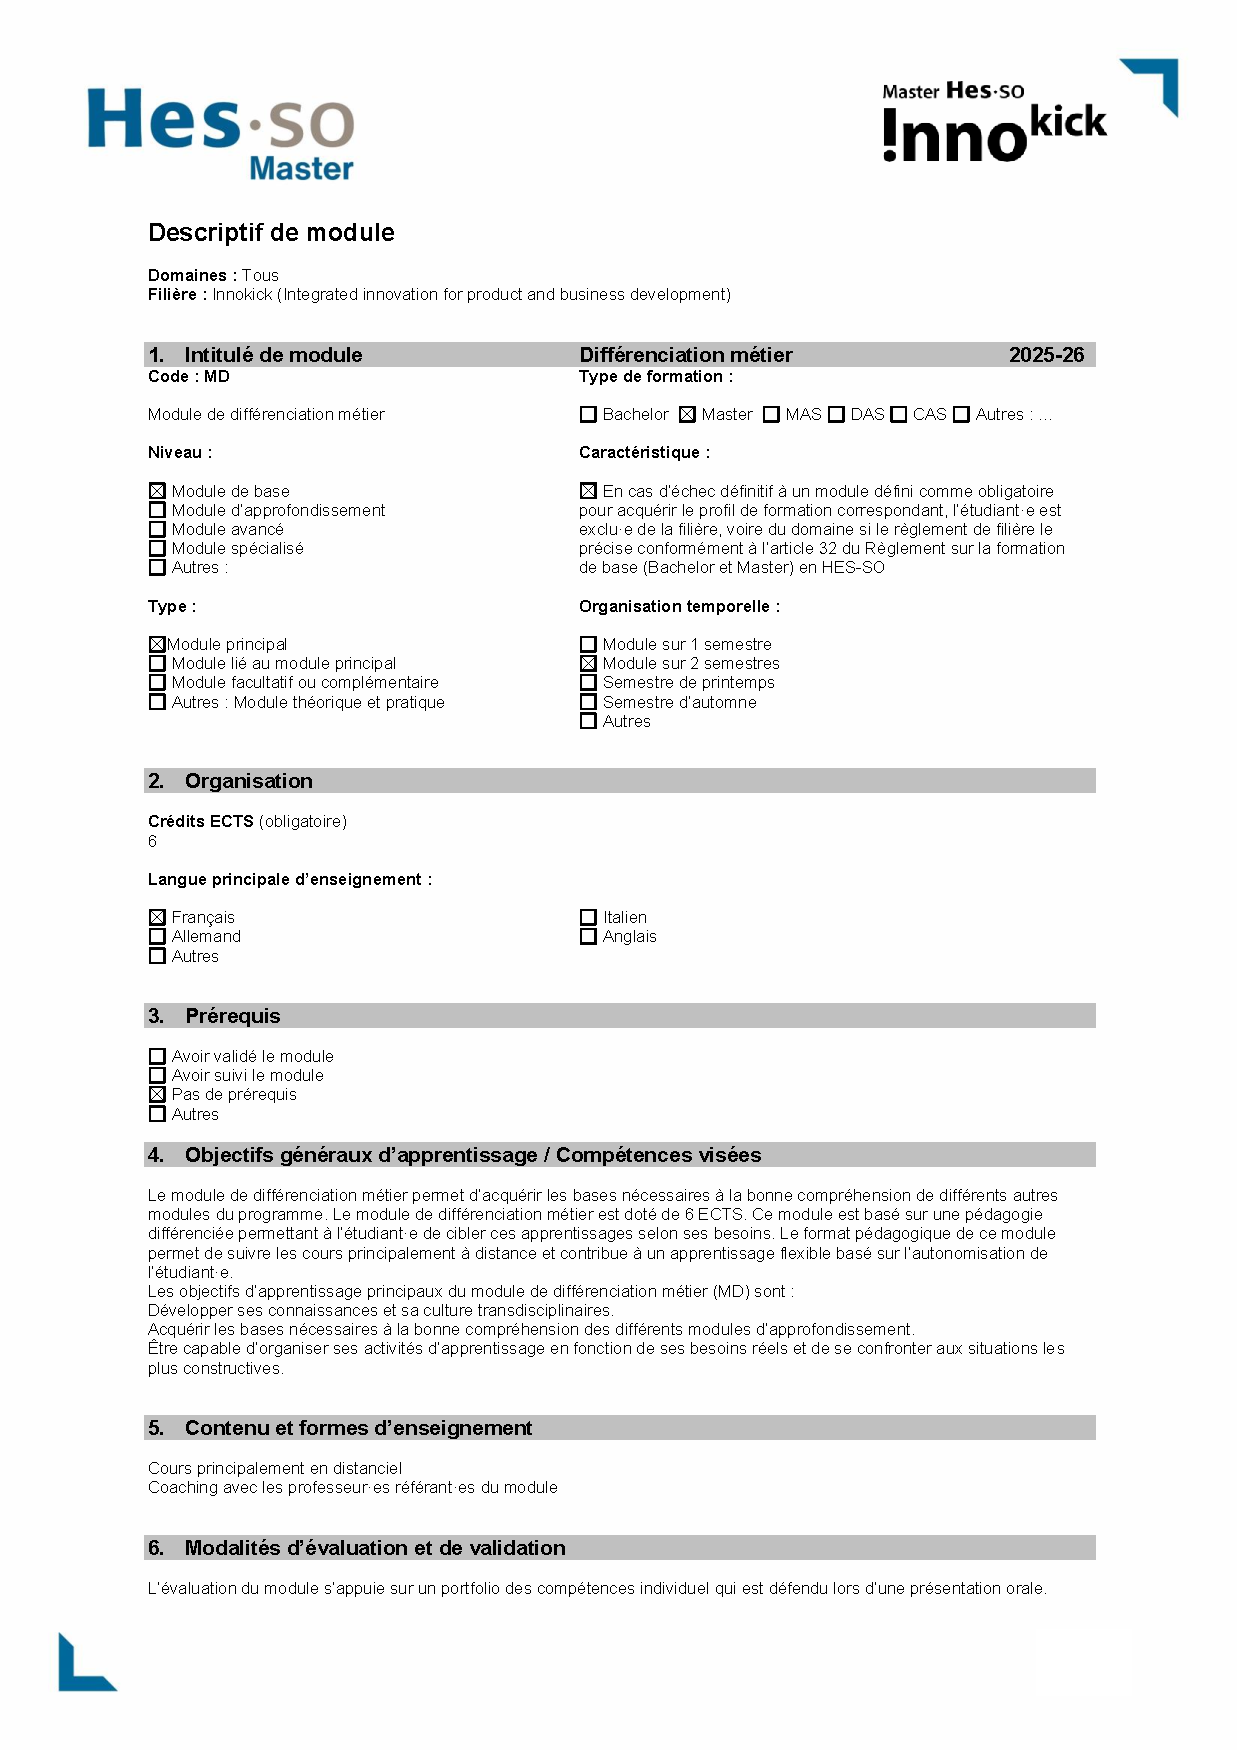
\includepdf[pages=-, pagecommand={\thispagestyle{annexepages}}]{annexes/pdfs/annexe-H-descriptif-mdm.pdf}

% : Annexe I : Plan d'Études Cadre (PEC) Master HES-SO Innokick ---
\chapter{Plan d'Études Cadre (PEC) : Master HES-SO Innokick (07.2024)}
\label{annex:pec-innokick}
\annexefiche
  {Version officielle juillet 2024 (document de référence programme)}
  {Cadre institutionnel global du Master HES-SO Innokick}
  {Fondement normatif des compétences, des phases Design Thinking et de la justification de périmètre (phase 6)}
  {Aucun caviardage (document institutionnel public)}

\includepdf[pages=-, pagecommand={\thispagestyle{annexepages}}]{annexes/pdfs/annexe-I-pec-innokick.pdf}

% : Annexe J : Glossaire technique ---
% =============================================================================
% ANNEXE J : Glossaire technique
% =============================================================================
% Consolide les définitions des termes techniques répétés dans le corps du
% portfolio (footnotes) afin d'alléger la lecture et de fournir une référence
% unique consultable de manière transversale.
% =============================================================================

\chapter{Glossaire technique}
\label{annex:glossaire}

\annexefiche
  {Consolidation produite en 2026 à partir des notes de bas de page du portfolio}
  {Référentiel transversal de vocabulaire technique utilisé dans les chapitres analytiques}
  {Lisibilité et précision terminologique (soutien transversal A2/B4/C2)}
  {Aucun caviardage (document pédagogique consolidé)}

Ce glossaire regroupe les définitions des termes techniques mobilisés dans le portfolio. Il vise à offrir une référence unique consultable de manière transversale, sans nécessiter le retour à chaque note de bas de page. Les termes sont classés par ordre alphabétique.

\bigskip

\begin{description}
  \item[\textbf{Agile (méthodes)}] Approches de gestion de projet fondées sur des cycles courts, la collaboration et l'adaptation continue. Elles privilégient des livraisons incrémentales plutôt qu'une planification figée.

  \item[\textbf{Architecture (logicielle)}] Organisation structurelle d'un système logiciel : découpage des composants, agencement, mise en relation, décisions techniques régissant leurs interactions (protocoles, interfaces, gestion des états).

  \item[\textbf{Artefact}] Document, outil ou livrable produit pendant l'action. Dans le cadre Tardif, sert de preuve observable de la compétence mobilisée.

  \item[\textbf{Backlog}] Liste priorisée des tâches, demandes et évolutions d'un projet. Mise à jour en continu selon les apprentissages et les contraintes.

  \item[\textbf{Board (agile)}] Représentation visuelle des tâches d'un projet, généralement structurée en colonnes (\textit{À faire / En cours / Terminé}). Donne une vue immédiate de l'avancement et des blocages.

  \item[\textbf{Branching}] Gestion des branches dans un système de versionnage : création de lignes de développement parallèles (typiquement une branche par fonctionnalité ou par version).

  \item[\textbf{Cascade (développement en)}] Approche séquentielle où chaque phase est clôturée avant la suivante. Risque principal : découvrir les erreurs tardivement, quand leur correction devient coûteuse. Synonyme : \textit{waterfall}.

  \item[\textbf{CI/CD}] \textit{Continuous Integration / Continuous Delivery (Deployment)}. Chaîne automatisée dans laquelle chaque modification de code déclenche la construction, les tests et, le cas échéant, le déploiement. Garantit que le code reste en permanence dans un état livrable et traçable.

  \item[\textbf{Commit}] Enregistrement d'un ensemble de modifications dans le système de versionnage, accompagné d'un message décrivant l'intention. Unité élémentaire de traçabilité du développement.

  \item[\textbf{Cycle de vie logiciel}] Ensemble des phases qu'un logiciel traverse, depuis l'expression du besoin jusqu'au retrait : analyse, conception, implémentation, vérification, validation, déploiement, maintenance.

  \item[\textbf{Definition of Done (DoD)}] Ensemble des critères qu'un livrable doit satisfaire pour être considéré comme terminé. En contexte médical, inclut le code, les tests, la documentation et la validation qualité.

  \item[\textbf{DevOps}] Ensemble de pratiques visant à rapprocher les équipes de développement (\textit{Dev}) et d'exploitation (\textit{Ops}), et à automatiser le cycle complet de livraison du logiciel.

  \item[\textbf{Exosquelette médical}] Dispositif mécatronique portable qui assiste ou remplace la motricité. En rééducation, guide les mouvements pour soutenir la reprise de la marche.

  \item[\textbf{Firmware}] Logiciel embarqué directement dans un composant matériel (microcontrôleur, carte électronique), au plus près du matériel. Pilote celui-ci en temps réel et n'est généralement pas modifiable par l'utilisateur final.

  \item[\textbf{Gate Review}] Revue de jalon. Point de contrôle formel à la fin d'une phase, durant lequel des critères prédéfinis sont vérifiés avant d'autoriser le passage à la phase suivante.

  \item[\textbf{GitLab}] Plateforme web intégrée de gestion de code source (basée sur Git) et d'industrialisation du développement logiciel : suivi des tickets, revues de code, intégration continue, registre d'artefacts.

  \item[\textbf{Hotfix}] Correction critique appliquée en urgence sur une version déjà livrée, en dehors du cycle normal de release.

  \item[\textbf{IEC 62304}] Norme internationale définissant les exigences relatives aux processus du cycle de vie des logiciels de dispositifs médicaux : développement, maintenance, gestion des risques, traçabilité. Obligatoire pour tout logiciel intégré dans un dispositif médical mis sur le marché européen.

  \item[\textbf{Ingénieur logiciel}] Professionnel qui conçoit, développe, teste, déploie et maintient des logiciels. À la différence du simple développeur, applique une démarche d'ingénieur : analyse formelle, choix raisonné d'architecture, prise en compte des contraintes de fiabilité, performance, sécurité et coût.

  \item[\textbf{Itératif}] Démarche procédant par cycles successifs produisant des livrables testables. Chaque cycle intègre des retours pour ajuster le suivant.

  \item[\textbf{JFrog Artifactory}] Gestionnaire d'artefacts logiciels : entrepôt centralisé qui stocke, versionne et trace les binaires produits par le développement (bibliothèques, paquets, images de conteneurs).

  \item[\textbf{KPI}] \textit{Key Performance Indicator}. Indicateur clé de performance, mesurant la pertinence d'un choix ou d'une activité selon des critères opérationnels explicites.

  \item[\textbf{Lean (méthode)}] Approche visant à maximiser la valeur produite tout en réduisant les gaspillages. En logiciel, privilégie des incréments utiles et rapides plutôt que des livraisons monolithiques.

  \item[\textbf{Livrable}] Tout produit, document ou artefact formellement remis à un destinataire (client, partie prenante, autorité réglementaire) au terme d'une activité ou d'un jalon.

  \item[\textbf{Logiciel embarqué}] Programme s'exécutant directement sur des composants matériels (microcontrôleurs, processeurs embarqués). Responsable du pilotage en temps réel, de l'acquisition des données capteurs et de la communication entre modules.

  \item[\textbf{MDR}] \textit{Medical Device Regulation} (Règlement UE 2017/745). Règlement européen sur les dispositifs médicaux, entré en application en mai 2021. Renforce les exigences en matière de sécurité, performance clinique, surveillance post-marché et traçabilité.

  \item[\textbf{Médiation}] Processus structuré où un tiers neutre aide deux parties à converger sans imposer de décision. Se distingue de l'arbitrage, où la décision est tranchée par une autorité.

  \item[\textbf{Pipeline (CI/CD)}] Chaîne d'étapes automatisées déclenchées à chaque modification du code source : compilation, tests, analyse de qualité, packaging, déploiement.

  \item[\textbf{Prototype}] Version partielle d'un produit destinée à tester une hypothèse de conception ou un besoin utilisateur. Niveau de fidélité variable selon l'objectif.

  \item[\textbf{Release}] Livraison officielle d'une version du logiciel, figée et traçable.

  \item[\textbf{Rétrospective}] Réunion de fin de sprint où l'équipe analyse ce qui a fonctionné, ce qui a bloqué, et les actions à mettre en place. Alimente l'amélioration continue.

  \item[\textbf{SAFe for Medical}] \textit{Scaled Agile Framework for Medical Devices}. Adaptation de SAFe aux contraintes réglementaires du médical, conciliant cadence agile et traçabilité normative.

  \item[\textbf{Scrum}] Cadre de travail (\textit{framework}) agile organisant le développement par sprints (2 à 4 semaines). Définit trois rôles (Product Owner, Scrum Master, Équipe), quatre événements (Planning, Daily, Review, Rétrospective), trois artefacts (Product Backlog, Sprint Backlog, Increment).

  \item[\textbf{SDP}] \textit{Software Development Plan}. Document de planification du cycle de vie logiciel obligatoire dans le contexte IEC~62304 (clause 5.1).

  \item[\textbf{SOUP}] \textit{Software of Unknown Provenance}. Composants logiciels tiers non développés en interne. En contexte médical, leur suivi (version, origine, risque, licence) est requis par IEC~62304.

  \item[\textbf{Sprint}] Période de travail courte et fixe (typiquement 2 semaines), au terme de laquelle l'équipe livre un incrément testable. Unité de base de Scrum.

  \item[\textbf{Sprint Planning}] Réunion d'ouverture du sprint durant laquelle l'équipe sélectionne les éléments du backlog et planifie le travail.

  \item[\textbf{Start / Stop / Continue}] Format de rétrospective en trois volets : ce qu'on commence, ce qu'on arrête, ce qu'on poursuit. Transforme le bilan en plan d'action concret.

  \item[\textbf{Template}] Gabarit. Modèle réutilisable qui standardise la structure d'un document. Son usage réduit le temps de production et les écarts de forme entre livrables.

  \item[\textbf{Timeboxing}] Attribution d'une durée fixe et non extensible à une activité. En facilitation, évite l'enlisement et force la production d'un résultat dans le temps imparti.

  \item[\textbf{V-Model}] Modèle de développement structuré en V. Branche descendante : conception (exigences, architecture, conception détaillée). Branche ascendante : validation par tests correspondants (unitaire, intégration, système, acceptance). Très utilisé en contexte réglementé.

  \item[\textbf{Vélocité}] En agile, quantité moyenne de travail (souvent mesurée en \textit{story points}) qu'une équipe parvient à terminer par sprint. Indicateur de capacité de production, non de valeur livrée.

  \item[\textbf{Versionnage}] Gestion systématique des différentes versions successives d'un fichier ou d'un logiciel. Permet de retrouver l'état exact à une date donnée, de comparer des versions, ou de revenir en arrière. Exigence fondamentale de traçabilité en contexte médical.

  \item[\textbf{Vote par points}] Méthode de sélection collective où chaque participant dispose d'un nombre limité de votes. La convergence s'appuie sur une agrégation des préférences du groupe.
\end{description}



% : Annexe K : Note opérationnelle d'usage de l'IA générative ---
% =============================================================================
% ANNEXE K : Note opérationnelle d'usage de l'intelligence artificielle générative
% =============================================================================
% Documente, conformément aux principes HES-SO (hessoIA2025) et UNESCO
% (unescoIA2022), l'usage concret de l'IA générative dans la rédaction du
% portfolio : modèles mobilisés, périmètre d'usage, périmètre d'exclusion,
% dispositif de vérification.
% =============================================================================

\chapter{Note opérationnelle d'usage de l'intelligence artificielle générative}
\label{annex:usage-ia}

\annexefiche
  {Synthèse rédigée en mai 2026, à la clôture du portfolio}
  {Documentation méthodologique interne sur l'usage de l'IA générative dans la rédaction}
  {Transparence académique et probité méthodologique (cadres HES-SO / UNESCO)}
  {Aucun caviardage (document déclaratif et méthodologique)}

\section*{Objet de l'annexe}

La sous-section \emph{Note méthodologique et choix de structure} du chapitre~\ref{chap:but_portfolio} déclare un recours à l'intelligence artificielle générative dans la rédaction du portfolio, encadré par les principes directeurs de la HES-SO~\citep{hessoIA2025} et la \emph{Recommandation sur l'éthique de l'intelligence artificielle} de l'UNESCO~\citep{unescoIA2022}. La présente annexe complète cette déclaration par une \textbf{description opérationnelle} de l'usage : quels modèles, pour quels usages, sur quel périmètre, avec quelles exclusions explicites, et selon quel dispositif de vérification. Elle vise à rendre auditable, par un examinateur exigeant, la frontière effective entre les apports de l'auteur et ceux des outils mobilisés.

\section{Modèles génératifs mobilisés}

Deux familles de modèles de langage ont été utilisées, de manière complémentaire :

\begin{itemize}
  \item \textbf{ChatGPT} (OpenAI), versions GPT-4 et GPT-4o, accessibles via l'interface conversationnelle publique, durant l'année académique 2025--2026.
  \item \textbf{Claude} (Anthropic), accessible via l'interface conversationnelle publique \texttt{claude.ai}, sur la même période.
\end{itemize}

Aucun modèle n'a été entraîné, finement ajusté (\emph{fine-tuned}) ni paramétré spécifiquement pour ce travail. Tous les usages relèvent de l'interaction par \emph{prompt} en langage naturel sur les versions standard accessibles au public.

Le choix de deux modèles distincts, plutôt que d'un seul, répond à un principe de \emph{contre-vérification croisée} : en cas de doute sur une formulation ou sur la solidité d'un argument, le passage était soumis aux deux modèles, et la convergence (ou la divergence) de leurs réponses informait la décision finale de l'auteur.

\section{Périmètre d'usage --- où l'IA a été mobilisée}

Les usages de l'IA ont été circonscrits à quatre catégories explicites :

\begin{enumerate}
  \item \textbf{Vérification de la cohérence argumentative entre sections.} Soumission de plusieurs sections à la fois pour identifier les contradictions internes, les répétitions et les enchaînements faibles. Exemple : alignement entre les compétences annoncées dans le contrat d'apprentissage et les preuves effectivement mobilisées dans le chapitre \emph{Situations}.
  \item \textbf{Audit et contre-argumentation.} L'IA a été instruite explicitement de jouer le rôle d'un évaluateur strict (par exemple, un examinateur de mémoire ou un spécialiste Tardif) afin d'identifier les faiblesses argumentatives. Les audits Tardif (\texttt{AUDIT\_TARDIF.md}) et académique (\texttt{AUDIT\_ACADEMIQUE.md}) ont été produits selon cette modalité ; leurs verdicts ont ensuite été révisés et arbitrés par l'auteur avant intégration au document.
  \item \textbf{Génération de tableaux structurés et de grilles.} Mise en forme tabulaire d'éléments dont le contenu était fourni par l'auteur : grilles Tardif synthétiques en tête de chaque compétence, grille de descripteurs de niveau (1--3 / 4--6 / 7--8 / 9--10), tableaux d'autoévaluation par famille. L'IA a produit la structure tabulaire ; l'auteur a fourni et validé les contenus.
  \item \textbf{Mise en forme \LaTeX{}.} Production et maintenance des environnements (boîtes \texttt{tcolorbox}, badges, en-têtes, footnotes complexes), des commandes personnalisées (\verb|\competences|, \verb|\caviarder|), et des graphiques TikZ (radars, chevrons). L'IA a accéléré la production typographique sans intervenir sur le contenu intellectuel.
\end{enumerate}

\section{Périmètre d'exclusion --- où l'IA n'a délibérément pas été mobilisée}

Les passages suivants ont été rédigés sans recours à l'IA générative, parce qu'ils relèvent de la \emph{voix réflexive personnelle} de l'auteur et que leur authenticité est constitutive de la valeur probante du portfolio au sens de~\citet{tardif2006} :

\begin{itemize}
  \item \textbf{Les autoévaluations chiffrées} (scores avant/après formation par dimension de compétence, dans les trois radars du \emph{Bilan de progression}) ainsi que leurs justifications individuelles. Toute médiation par un modèle de langage aurait introduit un biais de formulation incompatible avec l'exigence de probité méthodologique posée en section~\ref{sec:note-methodologique}.
  \item \textbf{Le récit des situations professionnalisantes} (faits, dates, personnes, déroulés). Les contextes bancaires, TWIICE et atelier Innokick relèvent de l'expérience directe : leur narration est strictement personnelle, anonymisée et synthétisée par l'auteur lui-même.
  \item \textbf{Les analyses réflexives en fin de chaque compétence} (sous-sections \emph{Analyse réflexive} et \emph{Apprentissages à entreprendre}). Ces passages relèvent de la pratique réflexive au sens de~\citet{schon1994} : ils ne peuvent être délégués sans dénaturer la démarche.
  \item \textbf{Le titre du portfolio et son argumentation} (chapitre~\ref{chap:titre_portfolio}). Le choix du titre \emph{Au-delà du code} et le récit du \emph{plafond technique} qui le soutient relèvent d'une décision rédactionnelle personnelle.
  \item \textbf{Le chapitre \emph{Perspectives pour la suite}} (chapitre~\ref{chap:perspectives}). Le projet professionnel et la lecture rétrospective des apprentissages ne peuvent venir que de l'auteur.
\end{itemize}

\section{Dispositif de vérification appliqué aux productions de l'IA}

Trois précautions ont été appliquées systématiquement aux passages où l'IA est intervenue :

\begin{enumerate}
  \item \textbf{Vérification factuelle des références bibliographiques.} Toute référence suggérée par un modèle de langage a été vérifiée auprès des sources primaires (catalogue éditeur, base de données ISBN, DOI) avant inclusion dans \texttt{references.bib}. Le risque de \emph{références hallucinées} est documenté dans la littérature ; il a été contré par cette étape de vérification, qui explique la modestie volontaire de la bibliographie (chaque entrée a été contrôlée).
  \item \textbf{Réécriture sur appropriation.} Les passages reformulés par l'IA ont été relus, retravaillés et appropriés par l'auteur : aucun texte n'a été inséré tel quel sans une lecture critique et, dans la majorité des cas, une réécriture partielle. La voix rédactionnelle du portfolio (registre, métaphores filées par chapitre, ponctuation) reflète des choix personnels que l'IA ne produit pas spontanément.
  \item \textbf{Contre-vérification croisée entre modèles.} Pour les passages sensibles (audit Tardif, audit académique, analyses réflexives complexes), la production d'un modèle a été soumise à l'autre pour identification des points faibles. Les éventuelles divergences ont été arbitrées par l'auteur.
\end{enumerate}

\section{Limites assumées de cette annexe}

Cette annexe ne prétend pas fournir un journal exhaustif des interactions avec les modèles. La traçabilité conversationnelle complète n'a pas été archivée de manière systématique. Trois limites doivent donc être assumées :

\begin{itemize}
  \item Le décompte précis du nombre d'interactions, du volume de tokens consommés ou du pourcentage de texte « touché » par l'IA ne peut être fourni.
  \item L'identification rétrospective des passages spécifiques où l'IA est intervenue est probabiliste, non déterministe : les listes des sections~3 et~4 décrivent des \emph{politiques d'usage} et des \emph{politiques d'exclusion}, non un marquage paragraphe par paragraphe.
  \item Pour les cycles d'écriture futurs, un journal d'usage daté et un système de marquage explicite des passages assistés par IA constitueraient une amélioration méthodologique souhaitable, conforme à l'évolution prévisible des standards académiques sur ce sujet.
\end{itemize}

\section{Conclusion : un usage encadré, non central}

L'IA générative a joué dans ce portfolio le rôle d'un \textbf{outil d'échafaudage} (au sens où l'on parle d'échafaudage en construction : on l'installe pour bâtir, on le démonte ensuite). Elle a accéléré la production des éléments accessoires (structure tabulaire, typographie \LaTeX{}, vérification de cohérence) et a fourni un partenaire de contre-argumentation pour les audits successifs. Elle n'a pas produit le contenu intellectuel central : sélection des compétences, identification des situations professionnelles, analyse des artefacts, lecture réflexive de la trajectoire. Cette frontière est revendiquée et défendable à l'oral : elle correspond, opérationnellement, à ce que les principes HES-SO appellent un usage \emph{« légitime et transparent »} de l'IA dans le cadre académique.


% : Annexe L : Note de pivot du contrat d'apprentissage ---
% =============================================================================
% ANNEXE L : Note de pivot du contrat d'apprentissage
% =============================================================================
% Reconstitution datée du basculement du 3e critère du contrat d'apprentissage
% (design / lecture de marché -> business layer / gouvernance de projet),
% conformément à l'exigence Tardif d'autorégulation tracée.
% =============================================================================

\chapter{Note de pivot --- glissement du 3\textsuperscript{e} critère du contrat d'apprentissage}
\label{annex:note-pivot}

\annexefiche
  {Note rédigée en mai 2026 (chronologie reconstituée a posteriori)}
  {Documentation réflexive du pivot entre contrat initial et trajectoire effectivement observée}
  {Autorégulation méthodologique : justification du glissement vers la \textit{business layer}}
  {Aucun caviardage (document réflexif ; limite assumée sur l'absence de trace contemporaine)}

\begin{tcolorbox}[colback=yellow!8, colframe=orange!70!black, boxrule=0.5pt, arc=3pt,
  left=8pt, right=8pt, top=6pt, bottom=6pt,
  title={\textbf{\small Statut de cette annexe}},
  fonttitle=\small\bfseries, coltitle=white, attach boxed title to top left={yshift=-2mm, xshift=4mm},
  boxed title style={colback=orange!70!black, arc=3pt, boxrule=0pt}]
\small
Cette note est une \textbf{reconstitution \emph{a posteriori}}, produite au moment de la rédaction finale du portfolio. Elle n'a pas été archivée en temps réel comme un point d'étape formel avec le professeur référent. Son statut est donc celui d'une \emph{rétrospective d'autorégulation} et non d'une trace contemporaine. Cette limite est explicitement assumée : elle est mentionnée dans la note méthodologique du chapitre~\ref{chap:but_portfolio} parmi les biais reconnus du dispositif, et identifiée par l'audit académique comme une faiblesse à corriger pour les cycles futurs (mise en place d'un journal de bord daté en cours d'année).
\end{tcolorbox}

\bigskip

\section*{1. Objet}

La présente note documente le basculement du \textbf{3\textsuperscript{e} critère du contrat individuel d'apprentissage} (cf.~annexe~\ref{annex:contrat-apprentissage}), initialement formulé en septembre 2025 comme \emph{« développer une conception centrée utilisateur et une meilleure lisibilité des solutions proposées »} (axe design / lecture de marché), vers un nouvel axe : \textbf{passage progressif vers la \textit{business layer}\footnote{Voir la note terminologique~\ref{fn:business-layer} dans le chapitre \textit{Perspectives}.} et la gouvernance de projet}, soutenu par la certification PRINCE2~\citep{prince2_2017}.

L'argumentation détaillée de ce pivot figure dans la section \emph{Pourquoi ce glissement par rapport au contrat d'apprentissage initial ?} du chapitre~\ref{chap:perspectives}. La présente annexe en restitue la chronologie, les déclencheurs et l'autorégulation associée.

\section*{2. Chronologie reconstituée}

\begin{tcolorbox}[colback=gray!5, colframe=gray!50, boxrule=0.4pt, arc=3pt,
  left=8pt, right=8pt, top=6pt, bottom=6pt]
\small
Les dates qui suivent sont reconstituées à partir des artefacts produits (note de décision, backlog, feuille de route, certification PRINCE2) et de la mémoire de l'auteur. Elles n'ont pas la précision d'un journal de bord tenu en temps réel.
\end{tcolorbox}

\smallskip

\begin{itemize}
  \item \textbf{Septembre 2025} --- Rédaction et validation du contrat d'apprentissage avec le professeur référent. Les trois axes retenus sont : (1) collaboration / délégation, (2) argumentation de valeur et lecture de marché, (3) conception centrée utilisateur et lisibilité des solutions. L'axe \emph{business layer / gouvernance} n'est \emph{pas} explicité comme tel ; il est latent dans l'axe~2.
  \item \textbf{Octobre--décembre 2025} --- Premiers mois de formation. Les cours \emph{Gestion de projet 1}, \emph{Méthodes de recherche 2} et \emph{Médiation scientifique} fournissent des outils que je commence à transposer dans l'environnement TWIICE. La première version de la note de décision technique (NDT-SW-001, annexe~\ref{annex:ndt-sw-001}) est produite. Première intuition : les compétences réellement mobilisées dans la pratique professionnelle relèvent davantage de la \emph{gouvernance décisionnelle} que du design d'interface.
  \item \textbf{Janvier 2026} --- Premier sprint adapté IEC~62304 chez TWIICE ; production du Software Development Plan (annexe~\ref{annex:sdp-markdown}). Constat : les artefacts qui produisent le plus de valeur dans ma pratique sont des artefacts de \emph{cadrage} (SDP, backlog priorisé, roadmap), non des artefacts de conception d'interface.
  \item \textbf{Février 2026} --- Préparation et passage de la certification PRINCE2~\citep{prince2_2017}, hors du périmètre prévu par le contrat d'apprentissage. Le passage se fait sur initiative personnelle, en lien avec un besoin perçu de \emph{cadre de gouvernance} pour structurer les arbitrages projet.
  \item \textbf{Mars 2026} --- \textbf{Point de bascule.} La conjonction des trois signaux (cohérence des artefacts produits, obtention de la certification PRINCE2, lecture en cours du chapitre Perspectives en cours de rédaction) fait apparaître que l'axe~3 du contrat d'apprentissage n'est plus le bon \emph{intitulé} de ce qui se développe réellement. Le mot juste n'est pas « design » mais \emph{gouvernance de projet et passage à la business layer}.
  \item \textbf{Avril--mai 2026} --- Documentation explicite de ce glissement dans le chapitre~\ref{chap:perspectives} du portfolio, et formalisation rétroactive de la présente note. Le contrat d'apprentissage initial n'est pas modifié (il reste l'engagement contractuel signé en septembre) ; le portfolio assume le décalage en l'explicitant.
\end{itemize}

\section*{3. Déclencheurs identifiés}

Trois éléments concourants ont rendu le pivot nécessaire :

\begin{enumerate}
  \item \textbf{Convergence des artefacts.} Les preuves accumulées au fil des compétences A2, B4 et C2 (note de décision, backlog priorisé, SDP, rétrospective, matrice de priorisation, roadmap) sont \emph{toutes} des artefacts de cadrage et de gouvernance. Aucune n'est un artefact de design d'interface. La lecture rétrospective de cette série révèle un axe que le contrat initial n'avait pas nommé.
  \item \textbf{Signal externe convergent (PRINCE2).} La préparation de PRINCE2, engagée pour des raisons indépendantes du portfolio, fait apparaître un alignement fort entre ses concepts (gouvernance par étapes, gestion des risques, tolérances, arbitrages) et la posture en construction.
  \item \textbf{Lecture critique du contrat initial.} L'axe~3 (« conception centrée utilisateur et lisibilité des solutions ») est apparu \emph{a posteriori} comme une formulation \emph{symptomatique} d'un manque plus structurant : non pas l'absence de capacité de design, mais l'absence de cadre de pilotage qui aurait permis à un éventuel design de trouver sa place dans une chaîne de décision crédible.
\end{enumerate}

\section*{4. Conséquences sur l'évaluation du contrat}

\textbf{Ce qui est conservé.} Les axes~1 (collaboration / délégation) et~2 (argumentation de valeur) du contrat sont maintenus tels quels. Les trois compétences certifiées (A2, B4, C2) restent celles définies dans le contrat. La logique d'alignement entre objectifs, compétences et choix de cours documentée au chapitre~\ref{chap:contrat_apprentissage} reste pertinente.

\textbf{Ce qui est déplacé.} L'axe~3 est \emph{recadré}, non remplacé. L'intention sous-jacente (renforcer une dimension qui me manquait à l'entrée en formation) est inchangée ; sa formulation devient plus juste à la lumière des apprentissages effectivement réalisés. Le design et la lecture de marché restent des angles de progression secondaires, non prioritaires pour la suite immédiate.

\textbf{Ce qui est explicitement assumé comme limite méthodologique.} Cette note de pivot n'est pas un point d'étape contractualisé en cours d'année. Elle ne porte pas la signature du professeur référent ; elle ne résulte pas d'une revue formelle datée. Pour les cycles d'apprentissage futurs, la mise en place d'un \textbf{journal de bord daté} et d'un \textbf{point d'étape semestriel contractualisé} constitueraient les améliorations méthodologiques permettant de produire des traces d'autorégulation \emph{contemporaines} plutôt que \emph{rétrospectives}.

\section*{5. Inscription dans le cadre Tardif}

Au sens de~\citet{tardif2006}, l'autorégulation est l'une des dimensions constitutives du portfolio d'apprentissage : l'étudiant doit pouvoir documenter \emph{comment} il ajuste sa trajectoire à la lecture de ses apprentissages effectifs. Cette annexe répond à cette exigence en restituant explicitement le glissement, ses déclencheurs et son arbitrage, plutôt que de le laisser apparaître seulement \emph{en creux} entre le contrat initial (annexe~\ref{annex:contrat-apprentissage}) et le chapitre~\ref{chap:perspectives}. La limite (reconstitution \emph{a posteriori} plutôt que trace contemporaine) est tenue comme l'un des biais explicitement assumés du dispositif, conformément à la note méthodologique du chapitre~\ref{chap:but_portfolio}.





% : Annexe M : Triangulation externe A2 -- extrait de courriel de convergence NDT ---
% =============================================================================
% ANNEXE M : TRIANGULATION EXTERNE A2 -- EXTRAIT DE COURRIEL DE CONVERGENCE NDT
% =============================================================================

\chapter{Triangulation externe : extrait de courriel attestant la convergence sur la NDT}
\label{annex:triangulation-a2-mail}

\annexefiche
  {Courriel professionnel produit chez TWIICE en 2026, postérieurement à la réunion d'alignement sur la NDT-SW-001 (horodatage exact caviardé)}
  {Message interne adressé par l'équipe Qualité/Affaires Réglementaires (QA/RA) aux parties prenantes de la réunion (R\&D, Software, l'auteur du portfolio)}
  {Triangulation externe de la \textbf{Preuve~1 de A2} (note de décision technique, annexe~\ref{annex:ndt-sw-001}) : un tiers atteste par écrit que la convergence a été obtenue et reconnaît la NDT comme référence partagée. Mobilisé en section A2.2 du chapitre \textit{Situations professionnalisantes}.}
  {Caviardage : expéditeur, destinataires nominatifs, fonctions précises, horodatage, références internes de projet et de procédure. Le contenu décisionnel est conservé intégralement.}

% : Note de mise en contexte (portfolio) -------------------------------------
\begin{tcolorbox}[colback=blue!5, colframe=blue!40!black, boxrule=0.5pt, arc=3pt,
  left=8pt, right=8pt, top=6pt, bottom=6pt]
  \small\itshape
  \textbf{Note du portfolio.} Cet artefact est un courriel professionnel réel,
  envoyé par l'équipe Qualité/Affaires Réglementaires (QA/RA) de TWIICE à
  l'issue de la réunion d'alignement portant sur la note de décision technique
  NDT-SW-001 (cf.~annexe~\ref{annex:ndt-sw-001}).

  Il atteste, par la parole écrite d'un tiers institutionnel distinct de
  l'auteur du portfolio, que la convergence revendiquée en section A2.2 a
  effectivement été obtenue et a été \emph{reconnue comme telle} par la
  fonction qualité, indépendante hiérarchiquement de l'équipe logicielle.

  Conformément aux règles de confidentialité de l'entreprise, l'expéditeur,
  les destinataires nominatifs, les fonctions précises et les références
  internes de projet ont été \textbf{caviardés}. Le contenu décisionnel
  (alignements, actions, points ouverts, prochaines étapes) est en revanche
  conservé \textbf{intégralement} : c'est lui qui porte la valeur probante.

  Au sens de Tardif, ce courriel transforme la triangulation externe pour A2
  d'un statut \emph{disponible mais non mobilisée} en un statut
  \emph{partiellement insérée et vérifiable}, sans avoir nécessité la
  divulgation d'informations confidentielles.
\end{tcolorbox}

\bigskip

% : Reproduction caviardee du courriel ---------------------------------------
\begin{tcolorbox}[enhanced, breakable, colback=gray!3, colframe=gray!55!black,
  boxrule=0.4pt, arc=2pt,
  left=12pt, right=12pt, top=10pt, bottom=10pt,
  title={\small\bfseries Courriel reproduit (caviardé)},
  fonttitle=\small\bfseries, coltitle=white,
  boxed title style={colback=gray!55!black, arc=2pt, boxrule=0pt}]

\small
\begin{tabular}{@{}p{2.4cm}@{\hspace{0.6em}}p{\dimexpr\linewidth-3cm\relax}@{}}
\textbf{De} & \caviarder[5.5cm] \hfill\textit{(QA/RA, TWIICE)} \\[2pt]
\textbf{À}  & \caviarder[5.5cm] \hfill\textit{(R\&D, Software, auteur)} \\[2pt]
\textbf{Date} & \caviarder[3cm] \\[2pt]
\textbf{Objet} & Compte-rendu de la réunion d'alignement NDT~--- décisions et actions \\
\end{tabular}

\medskip
\hrule
\medskip

Bonjour,

\medskip
Merci pour la réunion. Voici le résumé des points clés.

\medskip
\textbf{Décisions / alignements}
\begin{itemize}
  \item Convergence confirmée sur la NDT comme référence du besoin et point
        d'ancrage de la traçabilité.
  \item Accord pour aligner les exigences système et software sur la NDT,
        sans interprétations implicites. Toute divergence devra être justifiée
        et documentée.
\end{itemize}

\textbf{Actions}
\begin{itemize}
  \item QA/RA met à jour la matrice de traçabilité (NDT~$\rightarrow$~exigences
        $\rightarrow$~vérifications) pour refléter l'alignement.
  \item R\&D et Software relisent les passages encore ambigus et proposent une
        formulation finale.
\end{itemize}

\textbf{Points ouverts}
\begin{itemize}
  \item Arbitrage sur 2~formulations jugées ambiguës.
  \item Définition d'une date de gel (\emph{baseline}) de la NDT pour stabiliser
        la traçabilité.
\end{itemize}

\textbf{Prochaines étapes}
\begin{itemize}
  \item Mini-revue de clôture pour valider les deux formulations et acter la
        \emph{baseline}.
  \item Ensuite, lancement des mises à jour qualité associées.
\end{itemize}

\medskip
Cordialement,

\caviarder[4cm] \\
\caviarder[5.5cm] \hfill\textit{(QA/RA, TWIICE)}

\end{tcolorbox}

\bigskip

% : Lecture probante ---------------------------------------------------------
\section*{Lecture probante au sens de Tardif}

Quatre éléments du courriel constituent la valeur de triangulation~:

\begin{enumerate}
  \item \textbf{Émetteur tiers.} Le message est envoyé par la fonction QA/RA, hiérarchiquement distincte de l'équipe logicielle et institutionnellement responsable de la traçabilité IEC~62304. Sa parole engage l'organisation, pas l'auteur du portfolio.
  \item \textbf{Reconnaissance explicite de la convergence.} La formulation \emph{« Convergence confirmée sur la NDT comme référence du besoin et point d'ancrage de la traçabilité »} atteste, par un tiers, l'effectivité du résultat revendiqué en section A2.2 du portfolio. C'est la traduction écrite, postérieure à la réunion, du même fait que la NDT-SW-001 documente \emph{ex ante}.
  \item \textbf{Conséquences opérationnelles.} La distribution d'actions à QA/RA (matrice de traçabilité), R\&D et Software, ainsi que la planification d'une \emph{baseline}, montrent que la convergence n'est pas restée déclarative~: elle a déclenché des engagements de production documentaire chez d'autres équipes.
  \item \textbf{Lucidité sur les points ouverts.} La mention de deux formulations encore ambiguës à arbitrer témoigne de l'honnêteté du compte-rendu~: ce n'est pas un message de clôture triomphale mais un point d'étape équilibré, ce qui renforce sa valeur probante.
\end{enumerate}

\medskip
\noindent\textbf{Limite assumée.} Ce courriel est l'unique élément de triangulation externe matériellement inséré dans le portfolio. Les éléments équivalents pour B4 (historique GitLab, validations qualité du SDP) et C2 (feuille de route contresignée par la direction technique) restent \emph{disponibles sur demande motivée} mais non insérés (cf.~encart \emph{Triangulation externe} en tête du chapitre \textit{Situations professionnalisantes}). L'insertion d'un seul artefact suffit néanmoins à transformer le statut global de la triangulation externe d'une posture \emph{déclarative} à une posture \emph{partiellement insérée}, conformément à l'exigence Tardif de vérifiabilité par un tiers.

\clearpage



% =============================================================================
% AJOUTEZ VOS ANNEXES CI-DESSOUS EN SUIVANT LES EXEMPLES CI-DESSUS
% =============================================================================

\end{appendices}

\end{document}

